% warwickthesis.tex modified by M Hadley from utthesis.doc  Sept 96
% Significant changes were made in 2009, first to work seemlessly with pdflatex
% and secondly to use the setspace package to control linespacing -
% removing some incompatibilities that existed before.
% any comments or problems - contact me  <m.j.hadley@warwick.ac.uk>
%%%%%%%%%%%%%%%%%%%%%%%%%%%%%%%%%%%%%%%%%%%%%%%%%%%%%%%%%%%%%%%%%%%%%%%%%%%%%
%%%
%%% File: utthesis.doc, version 2.0, January 1995
%%% =============================================
%%% Copyright (c) 1995 by Dinesh Das.  All rights reserved.
%%% This file is free and can be modified or distributed as long as
%%% you meet the following conditions:
%%%
%%% (1) This copyright notice is kept intact on all modified copies.
%%% (2) If you modify this file, you MUST NOT use the original file name.
%%%
%%% This file contains a template that can be used with the package
%%% utthesis.sty and LaTeX2e to produce a thesis that meets the requirements
%%% of the Graduate School of The University of Texas at Austin.
%%%
%%% All of the commands defined by utthesis.sty have default values (see
%%% the file
%           warwickthesis.sty
%%%                        for these values).  Thus, theoretically, you
%%% don't need to define values for any of them; you can run this file
%%% through LaTeX2e and produce an acceptable thesis, without any text.
%%% However, you probably want to set at least some of the macros (like
%%% \thesisauthor).  In that case, replace "..." with appropriate values,
%%% and uncomment the line (by removing the leading %'s).
%%%
%%%%%%%%%%%%%%%%%%%%%%%%%%%%%%%%%%%%%%%%%%%%%%%%%%%%%%%%%%%%%%%%%%%%%%%%%%%%%
% all comments starting with %! have been added by M Hadley as
% part of the conversion for the university of warwick
%
%
%\documentclass[11pt,a4paper,twoside]{report}      %% LaTeX2e document.
%%* Removed twoside option which is no longer accepted - you might want to use it for drafts.
\documentclass[11pt,a4paper]{report}      %% LaTeX2e document.
%\documentclass[11pt,a4paper,draft]{report}      %% LaTeX2e document.
\usepackage{warwickthesis,setspace,graphicx}     %!  setspace is used to control linepacing
%\usepackage[square]{natbib}                    %! needed for Harvard style of references.
                                                %! for more notes see the bibliography section below
\usepackage{enumerate}  %! used for the library form, but you might find it useful too.
% \mastersthesis                     %% Uncomment one of these; if you don't
% \phdthesis                         %% use either, the default is \phdthesis.

%\thesisdraft                       %% Uncomment this if you want a draft
                                     %% version; this will print a timestamp
                                     %% on each page of your thesis.

%JR: it seems best not to uncomment any of these

% \leftchapter                       %% Uncomment one of these if you want
% \centerchapter                     %% left-justified, centered or
% \rightchapter                      %% right-justified chapter headings.
                                     %% Chapter headings includes the
                                     %% Contents, Acknowledgments, Lists
                                     %% of Tables and Figures and the Vita.
                                     %% The default is \centerchapter.

%\renewcommand{\familydefault}{cmss}  %! removed April 2009 because the default times font reads more easily
                                     %! for larger blocks of text.%!
                                     %! Added March 2003.
                                     %! This alternative is to use a sans serif font as in
                                     %!  the Warwick Corporate style.
                                     %! The default is Times, which is still acceptable.


\onehalfspacing                      %! This is the default and gives an acceptable "double spaced" thesis
                                     %! It is the minimum spacing accepted by the graduate school, and there is no reason to increase the spacing.
% \singlespacing                     %! Uncomment if you want single-spacing,
%\doublespacing                     %! uncomment if you want real double-spacing for some perverse reason.

%\setlength{\textheight}{9.0in}      %! Uncomment this for a slightly
                                     %! longer page. The default is now 8.5in (from Feb 2010)
                                     %! regulations require page numbers to be at least 1.5cm into the page.
                                     %! You can even try a longer page to save paper.

%! Double sided printing is no longer allowed (March 2008), it caused too many problems at binding,
                              %\setlength{\evensidemargin}{0.15in}  %! Uncomment this line for double sided printing
                                      %! Double-sided printing has recently been
                                      %! allowed by the Graduate School (March 2003)
                                      %! The default is {0.7in} for single sided.
%! Double sided printing is no longer allowed (March 2008), it caused too many problems at binding,

\renewcommand{\thesisdepartmentname}{Complexity Science and Statistics}    %! The name of
                                                  %   the department

%! \renewcommand{\thesissubmission}{Submitted to the University of Warwick\\
%!              in partial fulfilment of the requirements\\
%!                   for admission to the degree of\\}
%!
%!!!!!!!! default is:
%!
\renewcommand{\thesissubmission}{Submitted to the University of Warwick\\
                        for the degree of}
%!
%! In the title page this wording will be preceeded by:  thesis\\
%!                 and ended by:  Doctor of Philosophy   (or the
%!                                               selected alternative names
%! use \\ where you want a new line

\renewcommand{\thesisauthor} {Jeremy Francis Reizenstein}    %% Your official name.
\renewcommand{\thesisauthorno}{1359119}  %! your university number, used on the library copyright page.

%Month and year of submission
\renewcommand{\thesismonth}{September}     %% Your month of graduation.

\renewcommand{\thesisyear}{2018}      %% Your year of graduation.

\renewcommand{\thesistitle}{Iterated-Integral Signatures in Machine Learning}     %% The title of your thesis; use
                                     %% mixed-case.

%! \renewcommand{\thesistitletypesize}{\LARGE}   %! Put this in if you
                                  %!   want a Large title the default is \large

%This is optional
\renewcommand{\thesisauthorpreviousdegrees}{}
                                     %% Your previous degrees, abbreviated;
                                     %% separate multiple degrees by commas.

\renewcommand{\thesissupervisor}{Anastasia Papavasiliou}
                                     %% Your thesis supervisor; use mixed-case
                                     %% and don't use any titles or degrees.

%only used in VITA?
\renewcommand{\thesisauthoraddress}{}
                                     %% Your permanent address; use "\\" for
                                     %% linebreaks.
%%%%%%%%%%%%%%%%%%%%%%%%%%%%%%%%%%%
%! For the library declaration page only
%! \renewcommand{\thesiscopyrightagree}{agree}
                        %! agreement to allow single photocopies this is the default
%! \renewcommand{\thesiscopyrightagree}{do not agree}
                        %! refusal  to allow single photocopies

%! \renewcommand{\thesiscopyrightagreewhen}{immediately.}
                        %! that is the default to be used in all but the most exceptional circumstances
%! \renewcommand{\thesiscopyrightagreewhen}{after an embargo period of ……….................... months/years as agreed by the Chair of the Board of Graduate Studies.}
                         %! An alternative, if you have permission. Replace the .... month/years with approved period or change the wording to insert a date.

%! \renewcommand{\thesisinternetagree}{thesis can be made publicly available online.}
                         %! default online declaration for WRAP
%! \renewcommand{\thesisinternetagree}{thesis cannot be made publicly available online.}
                          %! use if necessary
%! \renewcommand{\thesisinternetagree}{thesis can be made publicly available only after…..}
                          %! conditional agreement, please put the date in place of the dots, ending with a fullstop.
%! \renewcommand{\thesisinternetagree}{full thesis cannot be made publicly available online, but I am submitting a separately identified additional abridged version that can be made available online.}



%%%%%%%%%%%%%%%%%%%%%%%%%%%%%%%%%%%%%%%%%%%%%%%%%%%%%%%%%%%%%%%%%%%%%%%%%%%%%
%%%
%%% The following commands are all optional, but useful if your requirements
%%% are different from the default values in utthesis.sty.  To use them,
%%% simply uncomment (remove the leading %) the line(s).

% \renewcommand{\thesisdegree}{...}  %% Uncomment this only if your thesis
                                     %% degree is NOT "DOCTOR OF PHILOSOPHY"
                                     %% for \phdthesis or "MASTER OF ARTS"
                                     %% for \mastersthesis.  Provide the
                                     %% correct FULL OFFICIAL name of
                                     %% the degree.

% \renewcommand{\thesisdegreeabbreviation}{...}
                                     %% Use this if you also use the above
                                     %% command; provide the OFFICIAL
                                     %% abbreviation of your thesis degree.

%\renewcommand{\thesistype}{Thesis}    %% Use this ONLY if your thesis type
                                     %! is NOT "Thesis"
                                     %% Provide the OFFICIAL type of the
                                     %% thesis; use mixed-case.

% \renewcommand{\thesistypist}{...}  %% Use this to specify the name of
                                     %% the thesis typist if it is anything
                                     %% other than "the author".

%%%
%%%%%%%%%%%%%%%%%%%%%%%%%%%%%%%%%%%%%%%%%%%%%%%%%%%%%%%%%%%%%%%%%%%%%%%%%%%%%


\input header.tex          %! Input declarations, new
                              %theorems etc.

\begin{document}

%TODO UNCOMMENT THIS
%\thesiscopyrightpage                 %! Generate the copyright page for the library.
%%%%%%%%%%% \thesiscopyrightpagehardcopyonly This only applies for a masters thesis that will not go online.

\def \alph#1{{\color{bluee}\mathbf{#1}}}

%%* Uncomment a ttitle page.
%%TODO choose which
%\thesistitlepage                     %% Generate the title page.
\thesistitlecolourpage           %! Generates a COLOUR title page.

%%* Start roman page numbering here for contents, etc
\pagenumbering{roman} %! Begins roman numerals start from page i.

\tableofcontents                     %% Generate table of contents.
\listoftables                      %% Uncomment this to generate list
                                     %% of tables.
\listoffigures                     %% Uncomment this to generate list
                                     %% of figures.
%\listofalgorithms

\begin{thesisacknowledgments}        %% Use this to write your
%  \input ack.tex                    %% acknowledgments; it can be anything
                                     %% allowed in LaTeX2e par-mode.

                                     %! This following is not needed, but you may like to add it.
%This \lowercase\expandafter{\thesistype} was typeset with
%\LaTeXe\footnote{\LaTeXe{} is an extension of \LaTeX. \LaTeX{} is
%a collection of macros for \TeX. \TeX{} is a trademark of the
%American Mathematical Society. The style package {\em warwickthesis} was
%used.} by \thesistypist.
Thank you very much to my supervisors Anastasia Papavasiliou and Benjamin Graham. Thank you to so many people for collaborations, conversations and advice, especially  Joscha Diehl, 
Terry Lyons, %ok, right?
Sina Nejad, Harald Oberhauser, Michael Pearce, Daniel Wilson-Nunn, and the Complexity crew; and to many for broader support including my parents.

Thank you for the support of the Complexity Science Doctoral Training Centre, The Alan Turing Institute\footnote{EPSRC grant EP/N510129/1} and the Engineering and Physical Sciences Research Council, and to their staff.
%Thank you also for Microsoft’s donation of Azure credits to The Alan Turing Institute, which provided CPU time for the work in \autoref{sec:lstmsig}.
Computing resources for the work in \autoref{sec:lstmsig} were provided through a kind Microsoft Azure for Research award to the Alan Turing Institute.
Thank you for helpful pointers from two anonymous reviewers.
\end{thesisacknowledgments}

\begin{thesisdeclaration}        %! Use this to declare the extent of
                 %! the original work,
                 %! collaboration, other published
                                 %! material etc.it can be anything
                                 %% allowed in LaTeX2e par-mode.
%Replace this text with a declaration of the extent of the original work,
%collaboration, other published material etc. You can use any \LaTeX\
%constructs.
This thesis is submitted to the University of Warwick in support of my application for the degree of Doctor of Philosophy. 
It has been composed by myself and has not been submitted in any previous application for any degree.
The material in \autoref{chap:math} and \autoref{chap:aoa} stems from a collaboration with Joscha Diehl at MPI Leipzig. Most of sections~\ref{sec:fkk}, \ref{sec:myInvariant} and \ref{sec:rotinv2d} appear in \cite{invariants} which we have published.
Sections \ref{sec:iisigintro} through \ref{sec:iisigConcl}, as well as parts of the introduction,  
appear in \cite{iisigPaper} with my original supervisor Ben Graham which has been submitted for publication.
\autoref{sec:lstmsig} stems from a collaboration with Harald Oberhauser.

\end{thesisdeclaration}


\begin{thesisabstract}               %% Use this to write your thesis
                                     %% abstract; it can be anything
                                     %% allowed in LaTeX2e par-mode.
%!  \begin{singlespace}       %! uncomment this if you need single spacing
%   \input abstract.tex       %!           don't forget the end spacing!
                                     %! It must fit on one page.
                                     %! single spacing and smaller
                                     %! font size
                                     %!  is allowed here.
%!   \end{singlespace}
The iterated-integral signature, or rough-path signature, of a path has proved useful in several machine learning applications in the last few years. This work is extended in a number of ways. Algorithms for computing the signature and log signature efficiently are investigated and evaluated, which is useful for many applications of signatures when working with large datasets. Online Chinese character recognition using signature features with recurrent neural networks is investigated. A recurrent neural network cell which stores its memory as the signature of a path is suggested and demonstrated on a toy problem. 

There is an essentially unique element of the signature of a path in space which, under transformations of the space, scales with volume. That element is characterised geometrically.

Given two features of curves, you can make a new one by taking the signed area of the 2d curve those two features make as a curve is traced out. A simple algebraic description of those features (which turn out to be signature elements) which can be formed from linear combinations of such combinations of total displacements is conjectured and worked towards. This is know as ``areas of areas''.
\end{thesisabstract}

%\begin{thesisabbreviations}       %! Use this to give a list of
                                   %! abbreviateons
                                   %! It can be anything
%\end{thesisabbreviations}         %! allowed in LaTeX2e par-mode.
                                   %!The following may be useful':
                     %!\begin{itemize}
                     %!     \item[symbol]descriptive text..
                     %!\end{itemize}

%\end{thesisabbreviations}
%!!!!!!!!!!!!!!!                     %% Begin your thesis text here; follow
                                     %% the report style and group your text
                                     %% in chapters, sections, etc. eg:
%%* don't need this with one-sided printing
%\newpage{\pagestyle{empty}\cleardoublepage} %! ensure that Chapter 1 starts on an odd
                                           %! page when using double sided printing.
%Don't need notation section, unless I do much with shuffle closure stuff
\iffalse%notation section
\section*{Notation}
When dealing with the tensor algebra and related concerns I often choose to adopt the notation of \cite{FLA}.

There are a couple competing claims for the use of the $\otimes$ symbol in a work such as this, because we are dealing with the tensor algebra. % and numerics based on it.
Besides when introducing the tensor algebra in 
%TODO
the symbol $\otimes$ is never used to indicate the product, otherwise known as the concatenation product, within the tensor algebra. It generally means the external tensor product, which produces (elements of) tensor powers of the tensor algebra. This is consistent with \cite{FLA}. But our $\otimes$ is what \url{https://en.wikipedia.org/wiki/Tensor_algebra} calls $\boxtimes$.
%In section \ref{sec:backprop}, the symbol has a concrete meaning as the kronecker product of vectors of numbers. - no we underline it there for clarity
\fi%notation section

\section*{Where is the code?}
\addcontentsline{toc}{section}{Where is the code?}
There has, naturally, been a lot of computer code involved in this project.
The good algorithms for signature and log signature calculations in \autoref{chap:iisig} have been released as part of the Python library \ii, whose homepage is at \url{github.com/bottler/iisignature}. 
From there, it should be easy to find its documentation and tests. Some associated tools etc.~are in the \verb|examples| subfolder.
Several other parts of this project have companion code in repositories of \url{github.com/bottler}, for example at \url{https://github.com/bottler/phd-code} and \url{https://github.com/bottler/free-lie-algebra-py}.

%%* Start arabic numbering of main text here
%I seem to be able to omit this
%\pagenumbering{arabic} %! Begins arabic numerals start from page 1.
\chapter{Introduction}
\ifx\headerIncludedJR\undefined
  \documentclass[11pt,a4paper]{article}
  \setlength{\textwidth}{5.50in}
  \usepackage[utf8]{inputenc}
\usepackage[T1]{fontenc}
\usepackage{amsmath}
\usepackage{amsthm}
\usepackage{amssymb}
%\usepackage{rotating}
%\usepackage{amslatex}
\usepackage{siunitx}
\usepackage{multicol}%for multicol
\usepackage{blkarray}%blockarray and block
\usepackage{comment}
\usepackage{fnbreak}%get a warning if a footnote is split
\usepackage[section]{placeins}
\usepackage{listings}
\lstset{breaklines=true,basicstyle=\ttfamily,language=Python}
\usepackage{arrayjobx}
\usepackage{array}%for \newcolumntype
%\usepackage[shortlabels]{enumitem}
\usepackage{mathtools}
\usepackage{afterpage}
\usepackage{setspace}% for \setstretch
\usepackage{algorithm}
\usepackage{algpseudocode}%for algorithmic
\usepackage{thmtools}%so that autoref works with Lemmas
\usepackage{tikz}
\usepackage{pgfplots}
\pgfplotsset{compat=1.15}
\usepackage{shuffle}
\usepackage{textcomp}%for \textrecipe
\usepackage{fontawesome}%for \faTable
\usetikzlibrary{calc,shapes,arrows.meta,decorations.markings,arrows}
\usetikzlibrary{graphs,positioning,svg.path,backgrounds}
\newcommand{\tikzmark}[1]{\tikz[overlay,remember picture] \node (#1) {};}
%\usepackage{CJKutf8}%for CJKChar

%\usepackage[backend=biber,backref=true]{biblatex}
\usepackage[backend=biber,style=alphabetic,backref=true,maxbibnames=10]{biblatex}
\addbibresource{sigs.bib}
\usepackage{url}

\usepackage{imakeidx}
%not a list of definitions, just symbols and abbreviations
%What is an abbreviation? Is QR? 
\makeindex[intoc,title=Symbols and abbreviations index]
\def\jind#1{\index{#1}}
\def\jindmath#1#2{\index{#2@$#1$}}
\def\jindv#1{\index{#1v@\texttt{#1}}}
%Some places I've given up and used \index in the text 
\definecolor{bluee}{rgb}{0.4, 0.4, 1.0}
%https://tex.stackexchange.com/questions/134191/line-breaks-of-long-urls-in-biblatex-bibliography
\setcounter{biburlucpenalty}{8000}
\setcounter{biburllcpenalty}{8000}

\usepackage{hyperref}

%so that autoref works with algorithms
\newcommand{\algorithmautorefname}{Algorithm}

%might help url breaking in bibliography
%\Urlmuskip=0mu plus 1mu minus 1mu
%also all the emergencystretch/looseness/fussy/sloppy
%to play with
%https://tex.stackexchange.com/questions/18505/how-to-use-sloppy-for-just-some-references

\def\ii{{\texttt{iisignature}}}
\def\pypi{{\texttt{PyPI}}}
\def\numpy{{\texttt{numpy}}}
\def\scipy{{\texttt{scipy}}}
\def\i#1{\index{#1@\texttt{#1}}}
\def \hilite#1{\underline{\color{blue}\textbf{#1}}}
%\def \alph#1{{\color{blue}\mathbf{#1}}}
\def \lex{<_L}
\def\kron{\underline{\otimes}}

\graphicspath{{C:/Users/Jeremy/Dropbox/phd/graphs/}{/home/jeremyr/Dropbox/phd/graphs/}{/Users/reizenstein/DropboxPersonalSymlink/phd/graphs/}}

%\RequirePackage{relsize}
%\DeclareRobustCommand\CXX{C\kern-.05em \raisebox{.3ex}{\scalebox{0.9}{\textbf{+\kern-.10em+}}}}
\DeclareRobustCommand\CXX{C\kern-.05em {\scalebox{0.9}{\textbf{+\kern-.10em+}}}}
%\DeclareRobustCommand\{\texorpdfstring{\CXX}{C++}}
\DeclareRobustCommand\CC{C\texttt{++}}
\def\bftab{\fontseries{b}\selectfont}
\newtheorem{theorem}{Theorem}
%\newtheorem*{theorem*}{Theorem}%bad idea, because you can't refer to it.
\newtheorem{definition}[theorem]{Definition}
%\newtheorem{outsideTheorem}[theorem]{Theorem}
\newtheorem{example}[theorem]{Example}
\newtheorem{conjecture}[theorem]{Conjecture}
\newtheorem{lemma}[theorem]{Lemma}
\newtheorem{proposition}[theorem]{Proposition}
\newtheorem{remark}[theorem]{Remark}

\newcommand{\area}{\mathsf{area}}
\newcommand{\Area}{\mathsf{Area}}
\newcommand{\emptyword}{\epsilon}
\newcommand{\ds}{d} % dimension of the signal
\newcommand{\TC}{T((\R^\ds))} % concat
\newcommand{\TS}{T(\R^\ds)} % shuffle
\newcommand{\GL}{\operatorname{GL}}
\newcommand{\SO}{\operatorname{SO}}
%\newcommand{\id}{\operatorname{id}}
\newcommand{\id}{\mathsf{id}}

\newcommand{\evaluatedAt}[1]{\,\raisebox{-.5em}{$\vert_{#1}$}}

\def\hssymbol{\mathbin{\succ}}
\def\hs#1#2{#1\hssymbol#2} %half shuffle
%\def\hs#1#2{z(#1,#2)} %half shuffle
\def\areab#1{\underline{\area}(#1)}
\def\areabb{\underline{\area}}
\newcommand{\R}{\mathbb{R}}
\newcommand{\Q}{\mathbb{Q}}
\newcommand{\C}{\mathbb{C}}
\newcommand{\N}{\mathbb{N}}
\newcommand{\spann}{\operatorname{span}}
\newcommand{\sign}{\operatorname{sign}}

\DeclareMathOperator*{\argmax}{arg\,max}
\DeclareMathOperator*{\argmin}{arg\,min}
\DeclareMathOperator{\softmax}{softmax}

%indicate that this file has been had
\def\headerIncludedJR{}
\def\endDocumentJR{}

%general hints
%https://homepages.inf.ed.ac.uk/imurray2/compnotes/latex.html

  %this cannot be in header.tex as it messes up
  %the thesis copyright page
  \def \alph#1{{\color{bluee}\mathbf{#1}}}
  \begin{document}
  \tableofcontents
  \def\endDocumentJR{\printindex \printbibliography[heading=bibintoc]\end{document}}
\fi

%\section{Introduction}
The signature is an object which is crucial in the mathematical theory of rough paths\cite{Lyons98}, and the calculations have proved to be useful in machine-learning applications, particularly classification problems where the data itself is a stream or a path in space, ranging from an application to online Chinese handwriting recognition in 2013 \cite{BEN} to skeleton-based human action recognition in 2017 \cite{action}. Other domains where the data has this form include signals from EEG and other medical monitors, sound and financial time series, where some set of numbers is varying in time. Often the samples can be noisy, can have varying length and both local and global structure can be important. A survey of such applications is given in \cite{OxSigIntro}. 
\section{Plan}
\newcommand{\jrmath}{$\square$}
\newcommand{\jralgo}{\faListOl}%needs font awesome
%\textrecipe %needs textcomp, BG says too Roman-looking, it's slightly amusing
\newcommand{\jrresults}{\faTable}%faTable needs font awesome
%\viewdata ?Checkedbox, some sort of pencil?
%?\StopWatchStart for timings?
%https://tex.stackexchange.com/questions/121865 
%https://tex.stackexchange.com/questions/400557/how-to-add-connected-graphs-to-a-table
%https://tex.stackexchange.com/questions/33787/how-do-i-create-separate-columns-in-latex-without-text-flow
%\newcommand*{\fullref}[1]{\hyperref[{#1}]{\autoref*{#1} \nameref*{#1}}}
\newcommand*{\fullref}[1]{\hyperref[{#1}]{\ref*{#1} \nameref*{#1}}}
%autoref, autopageref seem useful
%There are independent streams of progress made in this document in the use of signatures in machine learning.  
\autoref{fig:plan} indicates contributions in subsequent chapters: sections which contain mathematical results with \jrmath,
those which describe algorithms with \jralgo{}
and those containing the results of computer experiments with \jrresults. The remainder of this introductory chapter introduces the signature in more detail.

\newcommand{\tablenode}[2]{\tikz[baseline=(#1.base),remember picture]\node[inner sep=0pt,name=#1]{#2};}
\newcommand{\jrsp}{\hspace{1em}}
%\enlargethispage{3\baselineskip}
\begin{figure}[h]
%\renewcommand\arraystretch{1}
%\begin{center}
\centering
 \begin{tabular}{l}
\tablenode{t1}{\fullref{chap:math}}\\
\jrsp\tablenode{tm1}{\fullref{sec:fkk}} \jrmath\\
\jrsp\tablenode{tm2}{\fullref{sec:myInvariant}} \jrmath\\
\jrsp\tablenode{tm3}{\fullref{sec:rotinv2d}} \jrmath\ \jralgo\\
\tablenode{t2}{\fullref{chap:aoa}} \\
\jrsp\tablenode{ta1}{\fullref{sec:aoaLinearU}} \jrmath\\
\jrsp\tablenode{ta2}{\fullref{sec:aoaLinear2d}} \jrmath\\
\tablenode{t3}{\fullref{chap:iisig}}\\
\jrsp\tablenode{ti1}{\fullref{sec:sigs}} \jralgo\\
\jrsp\tablenode{ti2}{\fullref{sec:c}} \jralgo\\
\jrsp\tablenode{ti3}{\fullref{sec:s}} \jralgo\\
\jrsp\tablenode{ti4}{\fullref{sec:impl} \jralgo}\\
\jrsp\tablenode{ti5}{\fullref{sec:time} \jrresults}\\
\jrsp\tablenode{ti6}{\fullref{sec:mem} \jrresults}\\
\jrsp\tablenode{ti8}{\fullref{sec:backprop}} \jralgo\\
\tablenode{t4}{\fullref{chap:deep}}\\
\jrsp\tablenode{tc2}{\fullref{sec:chinese} \jralgo\ \jrresults\ }\\
\jrsp\tablenode{tc4}{\fullref{sec:lstmsig} \jralgo\ \jrresults\ }\\
\end{tabular}
\begin{tikzpicture}[remember picture, overlay]
\def\drawadjL#1#2{\draw [->] ($(#1.west)+(-1em,0)$) to[out=180,in=180,looseness=2  ] ($(#2.west)+(-1em,0)$);}
%\def\drawadjLD#1#2{\draw [dotted,->] ($(#1.west)+(-1em,0)$) to[out=180,in=180,looseness=2  ] ($(#2.west)+(-1em,0)$);}
\def\drawadjR#1#2{\draw [->] ($(#1.east)+(1em,0)$) to[out=0,in=0,looseness=2  ] ($(#2.east)+(0.5em,0)$);}
\drawadjL{ta1}{ta2}
\drawadjL{ti1}{ti4}
\drawadjL{ti2}{ti4}
\drawadjL{ti3}{ti4}
\drawadjR{ti4}{ti5}
\drawadjR{ti4}{ti6}
%\draw [dotted,->] (ti8) to[out=180,in=180,looseness=2  ] (tc2);
\begin{scope}[dotted]
\drawadjL{ti8}{tc4}
\drawadjR{ti4}{tc2}
\drawadjR{ti4}{tc4}
\end{scope}
\end{tikzpicture}
%\end{center}
  \caption[Plan of this document]{Plan of this document. Introductory sections to each chapter are omitted. Arrows indicate significant dependencies, with the dotted arrows indicating that although there is a logical dependency, the sections can be read independently. The fact the arrows are so few should be helpful.}
  \label{fig:plan}
\end{figure}

\section{What is the signature of a path?}

The iterated-integral signature of a smooth path is an infinite sequence of numbers. It is used in the mathematical theory of differential equations driven by paths. In these problems, a path is the driving signal for a certain type of system. It turns out that the signature is exactly the information about a path which you need to know in order to predict how the output of the system will behave, using a generalisation of Taylor's theorem. %solve a certain type of differential equation which depends on the path
It is natural that the signature would also be the right information to extract from a path if we want a machine-learning algorithm to understand the shape of the path.

A $d$-dimensional path is given by a function %$\gamma$ 
from an interval $[a,b]\subset\mathbb{R}$ to $\mathbb{R}^d$. 
We call $\mathbb{R}^d$ the \emph{ambient space} of the curve.
%The signature of $\gamma$ 
Its signature depends on the appearance of the path and the direction it was created, but not the speed at which it was created. If a path is modified by adding or removing a section which is exactly backtracked over, then its signature does not change \cite{HL}. If the path has a time dimension along which it always increases (for example it is the graph of a function of time) then exact backtracking is impossible and so any two different paths will have different signatures.%
\footnote{The signatures of two paths are the same iff they are \emph{tree-equivalent} \cite{HL} which means that they only differ in terms of adding or removing pieces which consist of exact backtracking.}
%\footnote{For paths which are continuously differentiable at all but finitely many places, such as the paths which we deal with in applications which are piecewise linear between a set of specified points, the signatures of two different paths which contain no exact backtracking will differ \cite{chen}. This property has been extended to general bounded variation paths by \cite{HL}, where two paths will have different signatures unless they are \emph{tree-equivalent}.}
%If two bounded variation paths are different then their signatures will be different, unless they have so-called \emph{tree-like equivalence}, which implies that at least one contains a section where the path exactly retraces itself.\cite{HL}
%\footnote{The case for paths which are continuously differentiable at all but finitely many places, which is true of the paths which we deal with in \ii, which are piecewise linear between a set of specified points which are specified by a set of points, is proved in \cite{chen}.}% The paths which we deal with in \ii, which are piecewise linear between a set of specified points, are automatically of bounded variation. %The fact that a signature cannot distinguish between two paths where the only difference is that one path contains an extra section which is backtracked over is due. %It is difficult for a writer to backtrack precisely, and so every character should be distinguishable through its signature.
%It is possible that approximate backtracking might lead to numerically unstable signatures.
%is this true?

The signature is divided into units called levels. We cannot store the whole signature of a path on a computer, rather we calculate a certain number of levels of it. 
The more levels of a signature are known, the more precisely the shape of the path is determined.
%Similar smooth curves have similar signatures.
If a path changes very slightly, the first few levels of its signature will also only change very slightly. If a path is moved (translated) but retains its shape, its signature will not change. 

%\subsubsection*{Simple example}
The number of elements of level $m$ of the signature of a $d$-dimensional path is $d^m$. They are the values of iterated integrals which consist of $m$ nested integrals, and they are labelled with $m$ numbers each corresponding to one of the dimensions. To distinguish these numbers which label the dimensions from other numbers, we write them bold and in blue. For example, a two-dimensional path might be given in coordinates as  $(\gamma_{\alph1}(t),\gamma_{\alph2}(t))$ as $t$ varies from $a$ to $b$. Its signature is a function denoted by $X^\gamma_{a,b}$\jindmath{X^\gamma_{a,b}}{X} from words made of the bold blue alphabet to real numbers. Level three of its signature has eight elements, called $X_{a,b}^\gamma(\alph{111})$, $X_{a,b}^\gamma(\alph{112})$ and so on. The one indexed by the word $\alph{122}$ is %written as
\begin{align}
X_{a,b}^\gamma(\alph{122})=\int_{t_1=a}^b\int_{t_2=a}^{t_1}\int_{t_3=a}^{t_2}d\gamma_{\alph1}(t_3)\,d\gamma_{\alph2}(t_2)\,d\gamma_{\alph2}(t_1).
\end{align}


In general, the signature can be defined inductively on the length of the word, as an element of one level of the signature of a path is an integral involving the signature of a varying portion of the path. The signature of the empty word is the single value in level 0, and it is defined to always be 1. If $w$ is a word and $i\in\{\alph{1},\alph{2},\dots,\alph{d}\}$ then $X^\gamma_{a,b}(wi)$ is defined as the Stieltjes integral $\int_a^bX^\gamma_{a,t}(w)\,d\gamma_i(t)$. In the simple case that $\gamma_i$ is differentiable, this is equal to $\int_a^bX^\gamma_{a,t}(w)\,\gamma_i'(t)\,dt$.
We also use the symbol $S(\gamma)_{a,b}$ for $X^\gamma_{a,b}$\index{S@$S(\gamma)$ and $S(\gamma)_{a,b}$}.
When the endpoints $(a,b)$ of a path $\gamma$ are clear, the signature $X^\gamma_{a,b}$ may be denoted $S(\gamma)$.%\jindmath{S(\gamma)}{S}.%
\footnote{Sometimes in analysis, the term \emph{signature} is used in a slightly different sense: the signature of a path $\gamma$ is the whole function $(c,d)\mapsto X_{c,d}^\gamma$, or something equivalent to it, not just that function's value on the path's endpoints.
%, and it is often denoted by $\mathbb{X}$ with the path denoted by $X$. 
This document does not use that sense of the word.}

The information in the first level of the signature is the total displacement of the path, i.e.~the direction and distance from its starting point to its ending point. The information which the second level of the signature adds is the \emph{signed area} of the path projected in each plane. Higher levels of the signature provide more detailed information about the path's shape.

%\subsection{More technical remarks about the signature}
%The signature is invariant on translations of the path. It is also invariant on reparametrizing the path. It may therefore be useful in defining a good representation function.
%The beginning of every signature is its zeroth level, which is always the number 1. Because this carries no information about the path, we are only concerned with the non-constant part of the signature, i.e.~all the rest. \ii\ never outputs this constant 1.


%\subsubsection*{Parsimonious definition}

%A path in $\mathbb{R}^d$ (with coordinate axes $x_{\alph1},x_{\alph2},\ldots,x_{\alph d}$) can be described by a continuous map $\gamma:[a,b]\to \mathbb{R}^d$ with $\gamma(t)=(\gamma_{\alph1}(t),\gamma_{\alph2}(t),\ldots,\gamma_{\alph d}(t))$. Its \textbf{signature} is a function from words written in the alphabet $\{\alph{1},\alph{2},\dots,\alph{d}\}$ to $\mathbb{R}$, denoted by $X^\gamma_{a,b}$. %Some example words are `$\alph1$', `$\alph2\alph1$' and `$\alph1\alph2\alph1$'.
%The signature can be defined inductively on the length of the word. The signature of the empty word is defined as 1. If $w$ is a word and $i\in\{\alph{1},\alph{2},\dots,\alph{d}\}$ then $X^\gamma_{a,b}(wi)$ is defined as $\int_a^tX^\gamma_{a,t}\gamma_i'(t)\,dt$. The  restriction of the signature to words of length $m$ is the $m$th \textbf{level} of the signature. It contains $d^m$ values.

%The signature is made up of a series of levels, one for each nonnegative integer. 
%Level $m$ can be thought of as taking values in $(\mathbb{R}^d)^{\otimes m}$, which is a $d^m$-dimensional real vector space. %, and consists of the $d^m$ values of integrals of the form 
%\begin{equation}
%\int_a^b\int_a^{t_1}\dots\int_a^{t_{m-2}}\int_a^{t_{m-1}}\,dx_{i_1}(t_m)\,dx_{i_2}(t_{m-1})\,\dots\,dx_{i_{m-1}}(t_2)\,dx_{i_m}(t_1),
%\end{equation}
%$\int_a^b\int_a^{t_1}\dots\int_a^{t_{m-1}}\,dx_{i_m}(t_m)\,\dots\,dx_{i_2}(t_2)\,dx_{i_1}(t_1)$
%where each $i_j$ is allowed to range over values in $\{\alph{1},\alph{2},\dots,\alph{d}\}$.
%In this form, the signature is seen to be an element of the tensor algebra $T(\mathbb{R}^d)=\bigoplus_{m=0}^\infty (\mathbb{R}^d)^{\otimes m}$. %Chen's identity is a convolution and the signature of a line segment is an exponential series.

%\subsection{Some properties of signatures}
%The signature of a path takes values in a submanifold of the tensor algebra. Any polynomial function of the signature is actually


\subsection{Displacement}
As mentioned, the first level of the signature of a path is just that path's total displacement vector. 
This is not a complicated thing, but in certain simple cases it may contain enough information about a path, or about a section of a path, to be used further.
For example, it is enough information about handwritten digits to make a significant guess as to what the digit is. 
The Pendigits dataset \cite{pendigits} collected the traces of many people writing the digits 0 to 9. 
Figure~\ref{fig:displacement} shows the displacement of 18 of each digit on a scatterplot, we see that many like digits are clustered together.

\begin{figure}
\includegraphics[trim=0pt 10pt 0pt 0pt, clip,width=0.8\textwidth]{displacementScatter.pdf}
%\includegraphics[width=0.8\linewidth, height=0.56\linewidth]{placeholder.jpg}
\caption[Displacement of the first stroke of handwritten digits from Pendigits]{\label{fig:displacement}Displacement (i.e.~level 1 of the signature) of the first stroke of the first 18 of each handwritten digit 0 to 9 from the training data of \cite{pendigits}. 
The bounding box of each digit is scaled to $[-1,1]^2$ so that the displacement lies in $[-2,2]^2$.}
\end{figure}

\subsection{Signed area}
\label{sec:signedArea}
For a two-dimensional path, the information carried by the first two levels of the signature is the total displacement of the path (in the first level, which is two numbers) and the signed area between the path and the straight line from its beginning to end. %(in the second level, a single number, written as a coefficient of $[\alph1,\alph2]$). 
%The log signature contains just these three numbers.
In higher dimensions, the second level of the signature gives the signed area of the path projected into any plane.
Figure~\ref{fig:sig-comp} shows this information for two straight lines in the plane and their combination, which contains area. 
For $d=1$, the signature does not contain any information beyond the total displacement of the path, and is therefore not interesting. 
$d$ should be considered as at least 2 in the mathematical results of this thesis.\footnote{This is not to say that our methods are inapplicable to one-dimensional \emph{data}. There are canonical ways to produce higher-dimensional paths from a path, for example adding a time dimension or a lead-lag transformation (e.g.~\cite{OxSigIntro}).}
\begin{figure}%[H]
%	\begin{center}
\centering
\begin{tikzpicture}

\begin{scope}[decoration={ %very thick?  thick?
	markings,
	%the xshift needs to be half the length, so that the arrow appears in the middle
	%https://tex.stackexchange.com/questions/222262/position-arrow-decoration-by-center-not-by-tip
	mark=at position 0.5 with {\arrow[xshift=2mm]{Latex[length=4mm,width=2mm]};}}
] 
\def\halfsize{1}
\def\halfskip{0.8}
\def\bottomrow{-\halfsize-\halfskip}
\def\size{\halfsize+\halfsize}
\def\startTwo{\size+\halfskip+\halfskip}
\def\startThree{\startTwo+\size+\halfskip+\halfskip}
\draw[postaction={decorate}] (0,\halfsize)--(\size,-\halfsize);
\node at (\halfsize,\bottomrow){$\binom{1}{-1}$,0};
\node at (\size+\halfskip,0) {\Huge$+$};
\draw[postaction={decorate}] (\startTwo,-\halfsize)--(\startTwo+\size,\halfsize);
\node at (\startTwo+\halfsize,\bottomrow){$\binom{1}{1}$,0};
\node at (\startTwo+\size+\halfskip,0) {\Huge$\to$};
%\fill [pattern=grid,pattern color=blue!20] %needs patterns tikzpackage
\fill [color=blue!11]
(\startThree,\halfsize)--(\startThree+\size,-\halfsize)--(\startThree+\size+\size,\halfsize)--cycle;
\draw[postaction={decorate}] (\startThree,\halfsize)--(\startThree+\size,-\halfsize);
\draw[postaction={decorate}] (\startThree+\size,-\halfsize)--(\startThree+\size+\size,\halfsize);
\node at (\startThree+\size,\bottomrow){$\binom{2}{0}$,$1$};
\end{scope}
\end{tikzpicture}
\iffalse
		\resizebox{14cm}{!}{\includegraphics{sig_from_1308_0371.pdf}}
		%\resizebox{14cm}{!}{hello I'm stuck}\resizebox{14cm}{3cm}{in a resizebox}	
%		\resizebox{14cm}{!}{
%			$1\alph1+1\alph2+0[\alph1,\alph2]$\qquad\quad $1\alph1-1\alph2+0[\alph1,\alph2]$\qquad\qquad\qquad\quad
%			$2\alph1+0\alph2-1[\alph1,\alph2]$\qquad\quad\ \ }
		\begin{minipage}{14cm}
			\hskip0pt plus0.6fil$\binom11,0$\hskip0pt plus1.2fil$\binom1{-1},0$\hfil\hfil$\binom20,-1$\hskip0pt plus0.6fil
		\end{minipage}
\fi
%		\resizebox{14cm}{!}{
%			$\qquad\binom11,0\qquad\qquad \binom1{-1},0\qquad\qquad\qquad\qquad\quad\binom20,-1\qquad\qquad\ \ $}
		%		\resizebox{14cm}{!}{
		%			$1\otimes(1,1)\otimes(\tfrac12,\tfrac12,\tfrac12,\tfrac12)$\quad\quad $1\otimes(1,-1)\otimes(\tfrac12,-\tfrac12,-\tfrac12,\tfrac12)$\qquad\qquad\quad\quad\ \
		%			$1\otimes(2,0)\otimes(2,-1,1,0)$\qquad\quad\ \ }
		%\caption{Concatenating paths and the corresponding $m=2$ log signatures, which consist of their total displacements (which are written as coefficients of $\alph1$ and $\alph2$) and the total signed area (which is written as a coefficient of $[\alph1,\alph2]$).\label{fig:sig-comp}}
		\caption[Displacement and signed areas when two lines are concatenated]{Concatenating paths and the corresponding total displacements  and total signed areas.\label{fig:sig-comp}}
%	\end{center}
\end{figure}

The following is an intuitive definition of the signed area of a path in the plane. For a smooth closed path, that is one which ends where it starts, the signed area is the sum of the signed areas of the regions bounded by the path, which is the area times the number of times the path goes round that region in an anticlockwise manner minus the number of times the path goes round it clockwise (i.e.~the winding number). For example, in the path shown in Figure~\ref{fig:winding}(a), regions whose areas count positively are labelled with a \raisebox{1mm}{\tiny\boldmath\color{red}$+$}, and negatively with a \raisebox{1mm}{\tiny\boldmath\color{red}$-$}. One region's area counts twice negatively; it is labelled with \raisebox{1mm}{\tiny\boldmath\color{red}$--$}. One enclosed region's area does not count at all, it is unlabelled. For a more general path, its signed area is the signed area of the closed path you get by joining it with a straight line from its end to its start.
\def\windingpoints{(0,0) (1,1) (3,1) (1.5,-1) (1,-1) (0.8,0.7) (1.3,1.6)(1.1,1.7)(0.9,1.4)(1.8,0.5)(2.8,-1.3)(3.6,0.2)}
\begin{figure}[H]
	\begin{center}
		\begin{tikzpicture}[font=\tiny\boldmath\color{red}]
		\begin{scope}[decoration={
			markings,
			%	mark=at position 0.08 with {\arrow{Latex[blue,length=2mm]};},
			mark=at position 0.08 with {\arrow{Latex[length=2mm]};},
			mark=at position 0.3 with {\arrow{Latex[length=2mm]};},
			%	mark=at position 0.44 with {\arrow{Latex[length=1mm]};},
			mark=at position 0.52 with {\arrow{Latex[length=2mm]};},
			mark=at position 0.68 with {\arrow{Latex[length=2mm]};},
			mark=at position 0.9 with {\arrow{Latex[length=2mm]};} 
		}
		%	mark=at position 0.5 with {\arrow{>}}}
		] 
		\node at (-0.4,1) {\normalsize\color{black}(a)};
		\draw [->,postaction={decorate}] plot [smooth cycle] coordinates {\windingpoints};
		\node at (0.5,.3) {$-$};
		\node at (1.4,-0.4) {$-$};
		\node at (1.3,0.4) {$--$};
		\node at (2.2,0.7) {$-$};
		\node at (1.07,1.1) {$-$};
		\node at (2.9,-0.4) {$+$};
		\node at (1.05,1.5) {$+$};
		\end{scope}
		%	\end{tikzpicture}
		%	\hspace{0.6in}
		%	\begin{tikzpicture}[font=\tiny\boldmath\color{red}]
		\begin{scope}[scale=1, shift={(5,0)}] %around (b) and (c)
		\begin{scope}[decoration={
			markings,
			mark=at position 0.4 with {\arrow{Latex[length=2mm]};}}
		%	mark=at position 0.5 with {\arrow{>}}}
		] 
		\node at (-0.3,1) {\normalsize\color{black}(b)};
		\draw [smooth,tension=1,postaction={decorate}] plot coordinates {(1.1,1.1)(0.5,0.7)(0,0)(1,-1) (1.8,0) (0.7,1.1)};
		%\draw [smooth,tension=0,postaction={decorate}] plot coordinates {(1.1,1)(0.5,0.7)(0,0)(1,-1) (1.8,0) (0.7,1.1)};
		\draw [blue, densely dotted] (1.1,1.1) -- (0.7,1.1);
		%\draw plot [smooth,tension=0] coordinates {(1,0.9)(0.5,0.5)(0,0.2)(0,0)(1,-1) (2,0) (1.2,1)};
		\node at (0.9,1.05) {$-$};
		\node at (0.9,0) {$+$};
		
		\begin{scope}[shift={(2,0)}]
		\draw [smooth,tension=1,postaction={decorate}] plot coordinates {(1,0.9)(0.5,0.8)(0,0)(1,-1) (2,0) (1.2,1)};
		\draw [blue, densely dotted] (1.2,1) -- (1,0.9);
		%\draw plot [smooth,tension=0] coordinates {(1,0.9)(0.5,0.5)(0,0.2)(0,0)(1,-1) (2,0) (1.2,1)};
		\node at (1,0) {$+$};
		\end{scope}
		\end{scope}
		\begin{scope}[shift={(5,0)},decoration={
			markings,
			mark=at position 0.24 with {\arrow{Latex[length=2mm]};}}]
		\draw [smooth, tension=1,postaction={decorate}] plot coordinates{(0.4,0.6)(0.4,0.3)(1,0)(1.5,-0.6)(1,-1)(0.5,-0.6)(1,0)(1.5,0.5)(1,1)(0.5,0.7)};
		\draw [blue, densely dotted] (0.5,0.7) -- (0.4,0.6);
		%\draw plot [smooth,tension=0] coordinates {(1,0.9)(0.5,0.5)(0,0.2)(0,0)(1,-1) (2,0) (1.2,1)};
		\node at (0.9,0.5) {$+$};
		\node at (1,-0.5) {$-$};
		\node at (0,1) {\normalsize\color{black}(c)};
		
		\end{scope}
		\end{scope}%around (b and c)
		\end{tikzpicture}	
		\caption[Demonstrations of signed area]{\label{fig:winding} (a) A complicated closed path showing the multiplicity of each region it contains, (b) two idealised handwritten digit 0s showing the completion into a closed curve and showing how the nature of the straight line completion has only a small effect on the area, and (c) an illustration of an idealised handwritten digit 8 showing why, although it is a large object, its area might be small due to cancellation of a positive and negative part.}
	\end{center}
\end{figure}


As an example of how the area can be useful in classifying the shape of the path, consider classifying handwritten digits 0 and 8. Usually these are written with a single stroke which ends near its beginning, so the displacement is insufficient for distinguishing them. This is reflected in Figure~\ref{fig:displacement} which shows the 0s and 8s near the origin and intermingled. However, the signed areas are statistically different. The figure 0 is typically formed from a single anticlockwise loop, generating a positive signed area, while the figure 8 contains two regions with opposite sign, leading to cancellation of signed area. The diagrams in Figure~\ref{fig:winding}(b) and (c) illustrate this. 
%The Pendigits dataset \cite{pendigits} collected the traces of many people writing the digits 0 to 9, and 
The histogram in Figure~\ref{fig:histogram80} shows how different the  signed areas of the first (and usually only) strokes of these digits are for the same Pendigits training data.
This clear separation is an illustration of the potential usefulness of the signature for machine learning.
\begin{figure}[H]
	\begin{center}
		\includegraphics[width=4.387in]{histogram80}
		\caption[Histogram of Pendigits 8 and 0 first stroke signed areas]{\label{fig:histogram80}Histogram of areas of the first stroke of each 0 and 8 in the training portion of the Pendigits dataset.}
	\end{center}
\end{figure}

I discuss later some extensions to the idea of signed area. In \autoref{sec:myInvariant} I discuss a generalisation of this concept of signed area to more than two dimensions, and in \autoref{chap:aoa} I discuss interpreting the whole signature, or large parts of it, as signed areas calculated recursively.

\section{Words}
\label{sec:words}
In this section I introduce some background algebraic structures which I refer to repeatedly later.
The main source for all this background is \cite{FLA}. An informal introduction is given in \cite{LOGSIG}.
Consider a set $\Sigma=\{\alph{1},\alph{2},\dots,\alph{d}\}$\jindmath{\alph{1},\alph{2},\dots,\alph{d}}{12345} of $d$ ``letters'' which has an ordering $<$\jindmath{<}{<}. I use these blue bold numbers as labels for the dimensions. %, such as the set of upper case letters $A,\dots,Z$ or the numbers $\alph{1},\alph{2},\alph{3}$. 
The set of words with entries in $\Sigma$\jindmath{\Sigma}{Sigma} is called the \emph{Kleene Star} of $\Sigma$ and is denoted by $\Sigma^*$\jindmath{\Sigma^*}{Sigmas}. 
The length of a word $u$ is denoted $|u|$\index{u@$\vert u\vert$}. %this is a special use of " to quote index characters 
The empty word is denoted by $\emptyword$\jindmath{\emptyword}{epsilon} and the concatenation of words $u$ and $v$ is written $uv$%; concatenation is an associative operation
. If a word $w$ is equal to $uv$ for some words $u$ and $v$, then $u$ is said to be a \emph{prefix} of $w$ and $v$ is said to be a \emph{suffix} of $w$. If $u$ and $v$ are both not empty then they are said to be a \emph{proper} prefix and suffix of $w$. For example $\alph{1}$ is a proper suffix of $\alph{3231}$, and a suffix but not a proper suffix of $\alph{1}$.
The ordering $<$ on $\Sigma$ can be extended to an ordering $\lex$ \jindmath{\lex}{< <}on $\Sigma^*$ called \emph{alphabetical order} or \emph{lexicographic order} in the usual way. (Specifically: $\emptyword\lex u$ if $|u|>0$. For letters $a$ and $b$ and words $u$ and $v$, $au\lex bv$ if $a<b$ or both $a=b$ and $u\lex v$.)

%\section{Free vector space}
The \emph{free (real) vector space} on the finite set $\Sigma$ is the real vector space with basis given by the elements of $\Sigma$. We will just call it $\mathbb{R}^d$. An element looks like $a_1\alph{1}+\dots+a_d\alph{d}$ for real numbers $a_1,\dots,a_d$.

%\section{Tensor algebra}
The \emph{tensor algebra} of the vector space $\mathbb{R}^d$,  $\TS$\jindmath{\TS}{T}, is the set of finite sums of real multiples of words, or equivalently the set of functions from $\Sigma^*$ to $\mathbb{R}$ which are zero for all but finitely many words, or equivalently the free vector space on $\Sigma^*$, $\R\langle\Sigma\rangle$. $\TC$\jindmath{\TC}{TT} denotes the  functions from $\Sigma^*$ to $\mathbb{R}$, or formal power series on $\Sigma$ considered as noncommuting, or equivalently the set of (possibly) infinite formal sums of real multiples of words, $\R\langle\langle\Sigma\rangle\rangle$.  The word $u$ in $\Sigma^*$ is identified with the function which takes $u$ to 1 and all other words to 0, or the expression $1u$. 
We are only ever interested in finite restrictions of these in order to do calculations, in particular we choose an integer $m$ and ignore all words with length longer than $m$. $T^{\underline m}(\mathbb{R}^d)$\index{Tm@$T^{\underline m}(\mathbb{R}^d)$} is the real vector space with basis given by words of length $m$ or less\footnote{this is known as $T^{(m)}(\mathbb{R}^d)$ in the notation of \cite{Lyons07}}. 
%The function on pairs of words which returns their concatenation if it has length $m$ or less and returns the zero element otherwise extends uniquely to a bilinear operation\footnote{i.e. linear in each argument} on $T^{\underline m}(\mathbb{R}^d)$, which is called the \emph{concatenation product}. 
%Given two words $w_1$ and $w_2$, their concatenation is the word $w_1w_2$
The concatenation of words is extended linearly to form bilinear\footnote{i.e.~linear in each argument} associative operations on $\TC$, $\TS$ and $T^{\underline m}(\mathbb{R}^d)$ called the \emph{concatenation product}.
(On $\TC$ this is well defined and doesn't involve calculating infinite sums because each word is only the concatenation of finitely many pairs of words.)
For example, in $T^{\underline 4}(\mathbb{R}^3)$,\footnote{because the concatenation of $\alph{132}$ and $\alph{21}$ is ignored}
\[(9\emptyword+7\,\alph{132})(2\,\alph{1}+4\,\alph{21})=18\,\alph{1}+36\,\alph{21}+14\,\alph{1321}.\]

Level $m$ of the signature can be thought of as taking values in $(\mathbb{R}^d)^{\otimes m}$, which is a $d^m$-dimensional real vector space. In this form, the signature is seen to be an element of $\TC$.
If $a\in\TS$ and $b\in\TC$ we can form the inner product $\langle a,b\rangle=\langle b,a\rangle$\index{<>@$\langle,\rangle$} in the word basis because this is only a sum over the finitely many terms in $a$. In this way $\TS$ is a set of linear maps $\TC\to\R$. If $a\in\TS$ and $X$ is a signature then the notations $X(a)$ and $\langle a,X\rangle$ are equivalent for the value of the signature on $a$.\footnote{There is a slight confusion with the term ``signature element'', as it is used for both the value of a signature on an $a\in\TS$ and also, sometimes, specifically for the value of a signature on a word.}

If $p$, $q$ and $r$ are real numbers with $p<q<r$ and $\gamma$ is a bounded variation path $[p,r]\to \R^d$ then the result (from \cite{chen}) known as \textbf{Chen's identity} states that \begin{equation}
X^\gamma_{p,r}(i_1i_2\ldots i_n) %$
=\sum_{j=0}^nX^\gamma_{p,q}(i_1i_2\ldots i_{j})X^\gamma_{q,r}(i_{j+1}i_{j+2}\ldots i_n).
\end{equation}
(The products indicated with ellipses can be empty, indicating the empty word, on which any signature takes the value 1.) 

Restricting up to level $m$, this means that 
\begin{equation}\label{eq:chenInIntro}
X^{\gamma,\underline m}_{p,r}=X^{\gamma,\underline m}_{p,q}X^{\gamma,\underline m}_{q,r},
\end{equation}
using the concatenation product in $T^{\underline m}(\mathbb{R}^d)$, where $X^{\gamma,\underline m}_{p,r}$ means the signature of $\gamma$ on $[p,r]$ up to level $m$.

%\subsubsection{Shuffle product}

Given two words $w_1$ and $w_2$, their shuffle product $w_1\shuffle w_2$ \jindmath{\shuffle}{sha} is the multiset of words which can be formed by interleaving them, including multiplicity, which we write as a polynomial on words. For example
\begin{align*}
\alph1\alph2\shuffle\alph3 &= \alph3\alph1\alph2+\alph1\alph3\alph2+\alph1\alph2\alph3
\end{align*}
This is extended linearly to a commutative and associative operation on $\TS$.

The signature $X$ of a bounded variation path obeys the following relation, for any $a,b\in\TS$, which is a consequence of integration by parts or the product rule for differentiation. (\cite{Ree}, see also \cite[Theorem 3.2]{FLA})
\begin{equation}\label{eq:shuffle}
X(a)X(b)=X(a\shuffle b)
\end{equation}
In particular, therefore, not every element of $\TC$ is the signature of a bounded variation path. For example, we see that $X(\emptyword)$ must be $1$. Allowed elements are those known as \emph{grouplike} elements.\footnote{This is equivalent to the remark in section~3.5.2 of \cite{FLA}.}


\section{What is the log signature of a path?}
\label{sec:logsigs}
The \emph{log signature} (\cite{Sidorova}, \cite{Lyons07}, also \emph{logarithmic signature}) is a compressed version of the signature. 
It carries the same information, but in a more compact way. 
It is also divided into levels. 
Up to level $m$, the log signature contains fewer numbers than the signature.
Any given set of values for these numbers actually gives the log signature of some path up to that level, whereas 
this is not the case for signatures, because there is some redundancy in the signature.
For example the first two levels of the signature of a two-dimensional path consists of $2+2^2=6$ numbers but we saw that this information is the path's total displacement and signed area, which can be stored in three numbers, which are exactly the first two levels of the log signature. In applications, the log signature might be less susceptible to roundoff error. The log signature is defined in terms of the signature, in a way analogous to logarithms of numbers, but can be calculated via an independent algorithm.

%Any machine learning example where log signatures beat signatures
 
 
%\section{Log Signatures}
The space $\TC$, in which the signature of a $d$-dimensional path lives, has a notion of logarithm (\cite{FLA}, chapter 3), given by 
\begin{equation}\label{eq:log}
\log(\emptyword+T)=\sum_{n\ge1}\frac{(-1)^{n-1}T^n}{n},\jind{log}
\end{equation}
where $T$ has no $\emptyword$ component, and a notion of exponential, given by 
\begin{equation}\label{eq:expDef}
\exp(T)=\emptyword+\sum_{n\ge1}\frac{T^n}{n!}.\jind{exp}
\end{equation}
In particular, these are well-defined operations which are inverses
\begin{equation}
\big\{x\in T^{\underline m}(\mathbb{R}^d) \mid \langle x,\emptyword\rangle=1\big\}
\underset{\log}{\overset{\exp}{\leftrightarrows}}
\{x\in T^{\underline m}(\mathbb{R}^d) \mid \langle x,\emptyword\rangle=0\}.
\end{equation}
%where powers are in the concatenation product
%The signature itself lies on a submanifold of tensor space.
%Calculating the log signature expanded
Let $S$ be the set which consists of the signature of every path in $\mathbb{R}^d$ truncated up to some level $m$.
$S$ is not the whole of the vector space  $T^{\underline m}(\mathbb{R}^d)$, although it does \textit{span}  $T^{\underline m}(\mathbb{R}^d)$
%\footnote{see Lemma 8 in \cite{JD}}. 
(see \cite[Lemma 8]{JD}). In fact, $S$ forms a lower-dimensional manifold. The 
logarithm operation %(\cite{FLA}, chapter 3) %$\log:T(\mathbb{R}^d)\to T(\mathbb{R}^d)$ is defined by $\log(1+T)=\sum_{n\ge1}\frac{(-1)^{n-1}T^n}{n}$. 
maps this manifold continuously one-to-one to a linear subspace of $T(\mathbb{R}^d)$.
%(Note: as formal series, it is not true that the logarithms of all signatures of paths without truncation form a linear subspace.)
The image of a signature under the logarithm or its representation in a basis of this subspace is called the \textbf{log signature}. %The log signature of a path up to level $m$ is determined by an easy calculation from its signature up to level $m$, and t
The logarithms of two signatures which agree up to level $m$ will agree up to level $m$, and so the phrase ``log signature of a path up to level $m$'' is unambiguous.
%The passage to the log signature can be considered an information compression or a dimensionality reduction. 

The subspace in which the log signature of a path in $\mathbb{R}^d$ up to level $m$ lives is equivalent to the free $m$-nilpotent Lie algebra of type $d$, $\mathfrak{n}_{d,m}$. The log signature is a completely compressed version of the signature up to the same level -- for every value in $\mathfrak{n}_{d,m}$, there is a path with that truncated log signature. It is a Lie algebra under the bracketing operation defined by $[a,b]=ab-ba$. A clear presentation of the background to this is found in \cite{LR}.

$\mathfrak{n}_{d,m}$ is a finite dimensional real vector space, but there is no single obvious basis for it. In order to use the log signature as an efficient representation of a path, we need to choose a fixed basis.
%We return the log signature in terms of a fixed basis, so that it can be used as an efficient representation of a path. 
There are two commonly used bases. They are both \emph{Hall bases}\cite{hall1950}. A Hall basis is made up of bracketed expressions, which are expressions involving letters combined with Lie brackets like $[\alph1,[\alph2,\alph1]]$, and it is determined by an ordering of all bracketed expressions.
\begin{itemize}
	\item The \emph{Lyndon basis}\cite{shirshov}. Each basis element is labelled with a Lyndon word on $\{\alph1,\alph2,\dots,\alph{d}\}$, which is a sequence which comes earlier in lexicographic order than any of its \emph{rotations}. (For example, the rotations of $\alph{2432}$ are $\alph{2243}$, $\alph{3224}$ and $\alph{4322}$. $\alph{2243}$ and $\alph{1213}$ are Lyndon words but $\alph{31}$ and $\alph{3224}$ are not.) %in which each Lyndon word is the foliage of exactly one basis element. Within each level, we order the basis elements so that their Lyndon words are in alphabetical order.
	\item The standard/canonical Hall basis, which we implement in such a way as to match CoRoPa\cite{coropa} exactly. %This basis still has the property that each element can be identified by its foliage
	The ordering of equal-length expressions $[A,B]$ and $[C,D]$ is defined recursively: $[A,B]<[C,D]$ if either $A<C$ or ($A=C$ and $B<D$).
\end{itemize}

In these bases, each basis element is either a letter or a single bracketed expression, whose left and right are basis elements. We always pick an order on basis elements such that shorter bracketed expressions come before longer ones, and single letters, which are the first level, are in their natural order $\alph1<\alph2<\dots<\alph{d}$.

From each bracketed expression we can form a word by deleting the brackets, which we call the expression's \emph{foliage}. For example the foliage of $[\alph1,[\alph2,\alph1]]$ is $\alph{121}$. Elements of a Hall basis are labelled by their foliages, which are called \emph{Hall words}. In the Lyndon basis the Hall words \emph{are} the Lyndon words.

In summary, the signature of a path is a special type of element of tensor space, called a grouplike one. It is the tensor exponential of a Lie element. 
This element is called the \emph{log signature} of the path.
Hall bases are practical bases for free nilpotent Lie algebras, which is where truncated log signatures take their values.
A Hall basis is graded, its elements in each level provide a basis for that level. Its elements in level $m$ are labelled with words of length $m$ called Hall words.
The term \emph{log signature} of a path is also used for the numerical expression in terms of a Hall basis.
If $h$ is a Hall word, we write $P_h$ for the corresponding Lie element.\jindmath{P_\cdot}{P}
%This notation assumes that a particular Hall basis is fixed. 

\subsection{Extracting a single log signature element from the signature}
\label{sec:usepi1adjoint}
Every polynomial function on signatures can be written uniquely as a linear combination of signature elements, i.e.~as a linear function on the signature. In particular, any element of the log signature can be written as an expression in terms of the signature. 
Here I present a simple way to find this expression.%, which was suggested by Joscha Diehl.

Considering everything up to level $m$, there is a unique linear map $\pi_1$\jindmath{\pi_1}{pi1} defined on the truncated tensor algebra which agrees on truncated grouplike elements with the logarithm function. This is explained on page 58 of \cite{FLA}. %It is not the easiest thing to calculate, but 
%We write down an expression for its transpose, which is efficient to calculate in practice.
(This is an example of the general principle that every polynomial function from grouplike elements / signatures to the reals extends uniquely to a linear function from $\TC$ to the reals. This reflects how much redundancy there is in the signature.).

%I note some local definitions from \cite{FLA}.
Denoting the non-empty words by $\Sigma^+$, $\pi_1$ of a word $w$ is given by 
\begin{align}
\pi_1(w)=\sum_{k\ge1}\frac{(-1)^{k-1}}{k}\sum_{u_1,\dots,u_k\in \Sigma^+}\langle w,u_1\shuffle\dots\shuffle u_k\rangle u_1\cdots u_k.\label{eq:pi1}
\end{align}
Its adjoint $\pi_1^\top$ \jindmath{\pi_1^\top}{pi1t}, which \cite{FLA} introduces in section 6.2 as $\pi_1^*$, is given by the similar expression, using the duality between shuffle and concatenation.
\begin{align}
\pi_1^\top(w)=\sum_{k\ge1}\frac{(-1)^{k-1}}{k}\sum_{u_1,\dots,u_k\in \Sigma^+}\langle w,u_1\cdots u_k\rangle u_1\shuffle\dots\shuffle u_k \label{eq:pi1adjoint}
\end{align}
This is explained in section~IV of \cite{Kawski}, where $\pi_1^\top$ is called $\pi_1'$.
$\pi_1^\top$ is easier to calculate than $\pi_1$ because its inner sum is simply over all decompositions of $w$ into $k$ words without having to think about preimages of the shuffle product.

For example,
\begin{align*}
\pi_1^\top(\alph{112})=\alph{112}-\frac12(\alph1\shuffle\alph{12}+\alph{11}\shuffle\alph2)+\frac13\alph1\shuffle\alph1\shuffle\alph2
\end{align*}

Fixing a Hall basis, there is a well known basis of each level of tensor space called the Poincar\'e-Birkhoff-Witt basis or PBW basis, described around page~91 of \cite{FLA}. Each basis element of level $m$ is indexed by a word of length $m$, we use the notation $P_w$\jindmath{P_\cdot}{P} for the element indexed by the word $w$. The PBW basis has the property that when $w$ is a Hall word then $P_w$ is the corresponding Lie element. 
Thus the notation here is consistent with our use of $P_w$ above when $w$ is a Hall word. 

On page~108 of \cite{FLA} is given an explicit construction of a dual basis $S$\jindmath{S_\cdot}{S} for the PBW basis. This is indexed by words, and if $w$ is a word then both $S_w$ and $P_w$ are elements of level $|w|$ of the tensor algebra. In particular, for any words $w$ and $w'$ we have that $\langle S_w,P_{w'}\rangle$ is 1 if $w=w'$ and zero otherwise.\footnote{Angle brackets are always the inner product in the word basis described in \autoref{sec:words}.}

%We can now 
%Let the log signature of a path be given by $l_\cdot$, i.e.~as $\sum_{h \text{ Hall}}l_hP_h$, and lets say we wish
Let's say we wish to find an expression for the log signature element corresponding to the basis element labelled with Hall word $h$.
If $X$ is the signature, then because its logarithm can be written as $\log X=\sum_{h' \text{ Hall}}l_{h'}P_{h'}$ for constants $l_\cdot$ and we are looking for $l_h$, our target is %we are actually looking for an expression for 
\begin{align}
\langle S_{h},\log X\rangle=\langle S_{h},\pi_1(X)\rangle=\langle \pi_1^\top(S_{h}),X\rangle
\end{align}
Thus $\pi_1^\top(S_{h})$ is exactly the expression we need.
This is not used in any of this work but is a possible alternative for obtaining the log signature whose performance could be investigated.

\subsection{An illustration}
  The log signature up to level 4 has 8 degrees of freedom. We can write it as tensors in the Lyndon basis in the following general form.%, writing $a\alph1$ as a short form for $aP_{\alph1}$ and so on.
\begingroup
\def\negjr#1{\ifnum\pdfstrcmp{0}{#1}=0 0 \else -#1\fi}
\def\pbinomjr#1#2{\left(\begin{smallmatrix}#1\\#2\end{smallmatrix}\right)}
\def\tr#1#2#3{\left(\begin{smallmatrix}#1\\#2\\#3\end{smallmatrix}\right)}
\def\ttr#1#2#3{\left(\begin{smallmatrix}0&#1&#3\\\negjr{#1}&0&#2\\\negjr{#3}&\negjr{#2}&0\end{smallmatrix}\right)}
\def\tttr#1{\left(\begin{smallmatrix}#1\end{smallmatrix}\right)}
\renewcommand\arraystretch{1.33}
\def\w#1{\makebox[\widthof{$\scriptstyle a^2b^2+4abc+12ae+12bd+214g-48g$}][c]{$\scriptstyle #1$}}
\begin{align}\begin{array}{c @{{}+{}} c @{{}+{}} c @{{}+{}} c}
    %a\alph1+b\alph2 & c\alph1\alph2 & d\alph1\alph1\alph2+e\alph1\alph2\alph2 & f\alph1\alph1\alph1\alph2+g\alph1\alph1\alph2\alph2+h\alph1\alph2\alph2\alph2\\
    aP_{\alph1}+bP_{\alph2} & cP_{\alph1\alph2} & dP_{\alph1\alph1\alph2}+eP_{\alph1\alph2\alph2} & fP_{\alph1\alph1\alph1\alph2}+gP_{\alph1\alph1\alph2\alph2}+hP_{\alph1\alph2\alph2\alph2}\\
    %a\alph1+b\alph2 & c[\alph1,\alph2] & \begin{matrix}d[\alph1,[\alph1,\alph2]]\\+\\e[[\alph1,\alph2],\alph2]\end{matrix} & f\alph1\alph1\alph1\alph2+g\alph1\alph1\alph2\alph2+h\alph1\alph2\alph2\alph2\\
    \pbinomjr{a}{b}& \tttr{0&c\\-c&0} & \tttr{\tttr{0&d\\-2d&e}\\\tttr{d&-2e\\e&0}} & \left(\begin{smallmatrix}\tttr{\tttr{0&f\\-3f&g}\\\tttr{3f&-2g\\0&h}}\\\tttr{\tttr{-f&0\\2g&-3h}\\\tttr{-g&3h\\-h&0}}\end{smallmatrix}\right)
\end{array}.\label{eq:arblogsig}
\end{align}
When exponentiated using \eqref{eq:expDef}, this expresses the signature truncated up to level 4 in the following form
\begin{align}
    &1+\pbinomjr{a}{b}+\tfrac12\left(\begin{smallmatrix}a^2&ab+2c\\ab-2c&b^2\end{smallmatrix}\right)
    +\tfrac16\tttr{\tttr{\makebox[\widthof{$\scriptstyle ab^2+6e+3bc$}][c]{$\scriptstyle a^3$}&a^2b+6d+3ac
      \\a^2b-12d& ab^2+6e+3bc}
    \\\tttr{a^2b+6d-3ac&ab^2-12e
      \\ab^2+6e-3bc&\makebox[\widthof{$\scriptstyle ab^2+6e+3bc$}][c]{$\scriptstyle b^3$}}}\nonumber
  \\&+\tfrac1{24}\left(\begin{smallmatrix}\tttr{\tttr{\w{a^4}&\w{a^3b+4a^2c+12ad+24f}\\a^3b-12ad-72f&a^2b^2+4abc+12ae+12bd+24g}\\\tttr{\w{a^3b-12ad+72f}&a^2b^2+4abc-24ae-24bd+12c^2-48g\\a^2b^2+24ae-12c^2&ab^3+4b^2c+12be+24h}}\\\tttr{\tttr{a^3b-4a^2c+12ad-24f&a^2b^2+24bd-12c^2\\a^2b^2-4abc-24ae-24bd+12c^2+48g&\w{ab^3-12be-72h}}\\\tttr{a^2b^2-4abc+12ae+12bd-24g&ab^3-12be+72h\\\w{ab^3-4b^2c+12be-24h}&\w{b^4}}}\end{smallmatrix}\right)\label{eq:arbsig}
\end{align}
Writing this out in terms of words would look like
\begin{align} \emptyword+a\alph1+b\alph2+\frac12\Big[a^2\alph{11}+(ab+2c)\alph{12}+(ab-2c)\alph{21}+b^2\alph{22}\Big]+\cdots
\end{align}
\endgroup

\endDocumentJR

\ifx\headerIncludedJR\undefined
  \documentclass[11pt,a4paper]{article}
  \setlength{\textwidth}{5.50in}
  \usepackage[utf8]{inputenc}
\usepackage[T1]{fontenc}
\usepackage{amsmath}
\usepackage{amsthm}
\usepackage{amssymb}
%\usepackage{rotating}
%\usepackage{amslatex}
\usepackage{siunitx}
\usepackage{multicol}%for multicol
\usepackage{blkarray}%blockarray and block
\usepackage{comment}
\usepackage{fnbreak}%get a warning if a footnote is split
\usepackage[section]{placeins}
\usepackage{listings}
\lstset{breaklines=true,basicstyle=\ttfamily,language=Python}
\usepackage{arrayjobx}
\usepackage{array}%for \newcolumntype
%\usepackage[shortlabels]{enumitem}
\usepackage{mathtools}
\usepackage{afterpage}
\usepackage{setspace}% for \setstretch
\usepackage{algorithm}
\usepackage{algpseudocode}%for algorithmic
\usepackage{thmtools}%so that autoref works with Lemmas
\usepackage{tikz}
\usepackage{pgfplots}
\pgfplotsset{compat=1.15}
\usepackage{shuffle}
\usepackage{textcomp}%for \textrecipe
\usepackage{fontawesome}%for \faTable
\usetikzlibrary{calc,shapes,arrows.meta,decorations.markings,arrows}
\usetikzlibrary{graphs,positioning,svg.path,backgrounds}
\newcommand{\tikzmark}[1]{\tikz[overlay,remember picture] \node (#1) {};}
%\usepackage{CJKutf8}%for CJKChar

%\usepackage[backend=biber,backref=true]{biblatex}
\usepackage[backend=biber,style=alphabetic,backref=true,maxbibnames=10]{biblatex}
\addbibresource{sigs.bib}
\usepackage{url}

\usepackage{imakeidx}
%not a list of definitions, just symbols and abbreviations
%What is an abbreviation? Is QR? 
\makeindex[intoc,title=Symbols and abbreviations index]
\def\jind#1{\index{#1}}
\def\jindmath#1#2{\index{#2@$#1$}}
\def\jindv#1{\index{#1v@\texttt{#1}}}
%Some places I've given up and used \index in the text 
\definecolor{bluee}{rgb}{0.4, 0.4, 1.0}
%https://tex.stackexchange.com/questions/134191/line-breaks-of-long-urls-in-biblatex-bibliography
\setcounter{biburlucpenalty}{8000}
\setcounter{biburllcpenalty}{8000}

\usepackage{hyperref}

%so that autoref works with algorithms
\newcommand{\algorithmautorefname}{Algorithm}

%might help url breaking in bibliography
%\Urlmuskip=0mu plus 1mu minus 1mu
%also all the emergencystretch/looseness/fussy/sloppy
%to play with
%https://tex.stackexchange.com/questions/18505/how-to-use-sloppy-for-just-some-references

\def\ii{{\texttt{iisignature}}}
\def\pypi{{\texttt{PyPI}}}
\def\numpy{{\texttt{numpy}}}
\def\scipy{{\texttt{scipy}}}
\def\i#1{\index{#1@\texttt{#1}}}
\def \hilite#1{\underline{\color{blue}\textbf{#1}}}
%\def \alph#1{{\color{blue}\mathbf{#1}}}
\def \lex{<_L}
\def\kron{\underline{\otimes}}

\graphicspath{{C:/Users/Jeremy/Dropbox/phd/graphs/}{/home/jeremyr/Dropbox/phd/graphs/}{/Users/reizenstein/DropboxPersonalSymlink/phd/graphs/}}

%\RequirePackage{relsize}
%\DeclareRobustCommand\CXX{C\kern-.05em \raisebox{.3ex}{\scalebox{0.9}{\textbf{+\kern-.10em+}}}}
\DeclareRobustCommand\CXX{C\kern-.05em {\scalebox{0.9}{\textbf{+\kern-.10em+}}}}
%\DeclareRobustCommand\{\texorpdfstring{\CXX}{C++}}
\DeclareRobustCommand\CC{C\texttt{++}}
\def\bftab{\fontseries{b}\selectfont}
\newtheorem{theorem}{Theorem}
%\newtheorem*{theorem*}{Theorem}%bad idea, because you can't refer to it.
\newtheorem{definition}[theorem]{Definition}
%\newtheorem{outsideTheorem}[theorem]{Theorem}
\newtheorem{example}[theorem]{Example}
\newtheorem{conjecture}[theorem]{Conjecture}
\newtheorem{lemma}[theorem]{Lemma}
\newtheorem{proposition}[theorem]{Proposition}
\newtheorem{remark}[theorem]{Remark}

\newcommand{\area}{\mathsf{area}}
\newcommand{\Area}{\mathsf{Area}}
\newcommand{\emptyword}{\epsilon}
\newcommand{\ds}{d} % dimension of the signal
\newcommand{\TC}{T((\R^\ds))} % concat
\newcommand{\TS}{T(\R^\ds)} % shuffle
\newcommand{\GL}{\operatorname{GL}}
\newcommand{\SO}{\operatorname{SO}}
%\newcommand{\id}{\operatorname{id}}
\newcommand{\id}{\mathsf{id}}

\newcommand{\evaluatedAt}[1]{\,\raisebox{-.5em}{$\vert_{#1}$}}

\def\hssymbol{\mathbin{\succ}}
\def\hs#1#2{#1\hssymbol#2} %half shuffle
%\def\hs#1#2{z(#1,#2)} %half shuffle
\def\areab#1{\underline{\area}(#1)}
\def\areabb{\underline{\area}}
\newcommand{\R}{\mathbb{R}}
\newcommand{\Q}{\mathbb{Q}}
\newcommand{\C}{\mathbb{C}}
\newcommand{\N}{\mathbb{N}}
\newcommand{\spann}{\operatorname{span}}
\newcommand{\sign}{\operatorname{sign}}

\DeclareMathOperator*{\argmax}{arg\,max}
\DeclareMathOperator*{\argmin}{arg\,min}
\DeclareMathOperator{\softmax}{softmax}

%indicate that this file has been had
\def\headerIncludedJR{}
\def\endDocumentJR{}

%general hints
%https://homepages.inf.ed.ac.uk/imurray2/compnotes/latex.html

  %this cannot be in header.tex as it messes up
  %the thesis copyright page
  \def \alph#1{{\color{bluee}\mathbf{#1}}}
  \begin{document}
  \tableofcontents
  \def\endDocumentJR{\printindex \printbibliography[heading=bibintoc]\end{document}}
\fi

\section{Tools}
Here I describe a number of new software tools for examining the signature which I have found useful, and which should help people in different ways trying to get to know the signature and its behaviour. They are not all original ideas.
\subsection{Five points in two dimensions}
\begin{figure}
	\begin{center}
		\includegraphics[width=0.8\textwidth]{MathematicaView2.png}
	\end{center}
	\caption[The \texttt{view.m} tool showing a path among five points.]{\label{fig:MathematicaView}The \texttt{view.m} tool showing a path among five points. The widgets on the right show its log signature up to level 8.}
\end{figure}
In the specific case $d=2$, $m=4$, the log signature has eight components, and a two dimensional path with four segments has eight degrees of freedom. The file \verb|view.m| provides an interactive Mathematica~10 visualisation of the relationship between a path made of four segments and its log signature. It depends on another file \verb|bch.m|, which has been generated by additional functionality in the original python logsignature code \cite{LOGSIG}, which defines a single function returning the log signature of a path defined by four displacements. The visualisation should appear when \verb|view.m| is run. The log signature appears as widgets on the right of the graph of the path. Because level 1 and level 3 of the log signature are two dimensional, they are represented by 2d controls. The other log signature components are controlled separately. When `solve' is ticked, you can gently move the widgets to change the components of the log signature and see the path move. Note that the $\alph{12}$ component controls the signed area enclosed by the path. The calculation of solutions is not perfect, but is enough to get a general picture. It is relying on built-in nonlinear optimisation routines in Mathematica to attempt to invert the signature in this special case.
%TODO: this should use polynomial methods instead. see the Polynomial Systems guide
When `solve' is unticked, you can drag the locators to change the path, and see the corresponding log signature elements move. For example, after drawing 3 paths the window might look as shown in \autoref{fig:MathematicaView}.

\subsection{Freehand drawing}
The simple tool \verb|freehand_draw.py| lets you draw paths with your mouse in a blank window. The signature of each path is printed on the console. This is one tool I wanted to have in order to get a feel for the signature elements. Signed area and its robustness on paths which are nearly closed is particularly easy to illustrate with the tool.

For example, after drawing 3 paths the window might look as shown in \autoref{fig:hey}.
\begin{figure}
%	\includegraphics[trim=0pt 10pt 0pt 0pt, clip,width=0.8\textwidth]{hey.gif}
\begin{center}
	\includegraphics{hey.png}
\end{center}
\caption{\label{fig:hey}Appearance of \texttt{freehand\char`_draw.py} after some mouse drags.}
\end{figure}
The following would be printed on the console, indicating truncated log signatures up to level 3 of each path. In particular, the three lines in order correspond to (1) the letters of the word `hey', (2) the vertical stroke of the exclamation mark and (3) the dot.
%\begin{quotation}
\begin{lstlisting}
[ 0.366492 -0.379581  0.020182 -0.007912 -0.003532]
[-0.002618 -0.212042  0.001631 -0.000008 -0.000014]
[ 0.002618  0.005236  0.000154  0.000001  0.000001]
\end{lstlisting}
%\end{quotation}

\subsection{Arbitrary precision signature calculations}
The \ii\ project sources include a project \verb|arbprec| which calculates signatures of paths in arbitrary precision and compares them to those using floating point arithmetic. Very often we see that these results do not differ by much for random paths. There are cases where calculating the signature of a path naturally results in a loss of floating point accuracy, for example the 1-dimensional path $(0),(a),(b)$ where $a\approx1$ and $b\approx0$, and so testing with arbitrary precision may be useful.
Long paths given by lots of points could create a unique problem, with this type of cancellation happening in some dimensions.
%Could illustrate this in mathematica with a long path that backtracks

\subsection{Free lie algebra calculations}

The file \verb|free_lie_algebra.py|\footnote{\url{github.com/bottler/free-lie-algebra-py}} provides objects to do many of the calculations described in \cite{FLA}. The main types are summarised in \autoref{tab:flaTypes}. It is useful for getting intuition and testing out conjectures, and is generally hackable.

As an example, we could try to find the linear combination of signature elements corresponding to the coefficient of $\alph{112}$ in the log signature in the Lyndon basis. We might do that like this using the method of \autoref{sec:usepi1adjoint}.
\begin{quotation}
\begin{lstlisting}[language=Python]
from free_lie_algebra import *
d=2
m=3
H=HallBasis(d,m,lessExpressionLyndon)

with UseRationalContext():
    answer=pi1adjoint(S("112",H))
\end{lstlisting}
\end{quotation}
This sets \verb|answer| to the \verb|Elt| representing $\pi_1^\top(S_{\alph{112}})$ which is what we are looking for.
If we run \lstinline[language=Python]{print(answer.pretty())} we will be told 
\begin{quotation}
	\begin{lstlisting}
	[1/6]112-[1/3]121+[1/6]211
	\end{lstlisting}
\end{quotation}
which fits with what we would come up with by staring at \eqref{eq:arbsig} to find a (in fact, the \emph{unique}) linear combination of elements which adds up to $d$, namely that
\begin{align*}
\def\b{\Big}
d=\frac16\b(\frac{a^2b+6d+3ac}{6}\b)-\frac13\b(\frac{a^2b-12d}{6}\b)+\frac16\b(\frac{a^2b+6d-3ac}{6}\b).
\end{align*}
%Without \verb|UseRationalContext|, the library uses its floating point numbers as the coefficients, which is less pretty.
The library uses floating point numbers as coefficients by default. The use of \verb|UseRationalContext| makes it use rational numbers from \verb|sympy| \cite{sympy}, which is prettier in a case like this.

We can further verify this in the code. The \verb|arbitraryGrouplikeEltSympy| function returns an arbitrary truncated signature expression as an \verb|Elt| in the style of \eqref{eq:arbsig}.
The coefficients are \verb|sympy| expressions. 
It is a tensor where each element in terms of its corresponding log signature elements for a given Hall basis.
Instead of labelling the log signature elements with letters of the alphabet like the $a,b,c,\dots$ of \eqref{eq:arblogsig}, the element corresponding to a word is given a name \verb|x| subscripted with the number which looks like the word. For example $c$ is \verb|x_12|.
We can perform the verification like this
\begin{quotation}
\begin{lstlisting}[language=Python]
    sig = arbitraryGrouplikeEltSympy(H)
    print(dotprod(sig,answer).expand())
\end{lstlisting}
\end{quotation}
which prints \verb|x_112| as desired.

%The alphabet $A$ is \verb|int| starting from 1. %The scalars are \verb|int| or \verb|float|, but this is made easy to change. The main types are listed in Table~\ref{tab:flaTypes}. Addition and scalar multiplication are overloaded, and the other main functions in Table~\ref{tab:flaOps}. The \verb|test()| function serves as a demonstration.
\begin{table}
\begin{tabular}{lp{3.4in}}
%\begin{tabular}{ll}
name&set\\%&comment\\
\hline
\verb|Word|&$\Sigma^*$\\
\verb|Elt|&tensor space, $K\langle \Sigma\rangle$\\
\verb|EltElt|&$K\langle \Sigma\rangle^{\otimes n}$, any $n$\\
\verb|tuple(int...)|&free magma, $M\langle \Sigma\rangle$\\
\verb|HallBasis|&a Hall basis for a given dimension and depth/level.\\
\verb|TensorSpaceBasis|&a basis of $K\langle \Sigma\rangle$, e.g.~the PBW basis or its dual, up to a given dimension and depth/level.
\end{tabular}
\caption{\label{tab:flaTypes}Types in \texttt{free\symbol{95}lie\symbol{95}algebra.h}}
\end{table}
\iffalse
\begin{table}
\begin{tabular}{lll}
function name&\pbox{2.4cm}{mathematical\\symbol}&comment\\\hline
\verb|concatenate|&&(concatenate words)\\
\verb|concatenationProduct|&&(concatenation product of \verb|Elt|)\\
\verb|concatenationProductEltElt|&&(concatenation product of \verb|EltElt|)\\
\verb|shuffleProduct|&$\shuffle$\\
\verb|tensorProduct|&$\otimes$\\
\verb|tensorProductFunctions|&$f_1\otimes f_2\otimes\dots$&where $f_i:\verb|Elt|\to\verb|Elt|\;\mathrm{or}\;\verb|EltElt|$\\
\verb|lieProduct|&$[\cdot,\cdot]$\\
\verb|dotprod|&&inner product of \verb|Elt| in basis of words\\
\verb|distance|&&distance between \verb|Elt|s in basis of words\\

\verb|conc|&conc and $\mathrm{conc}_p$\\
\verb|sh|&sh\\
\verb|sh_p|&$\mathrm{sh}_p$\\
\verb|epsilon|&$\varepsilon$&constant term of tensor\\
\verb|delta|&$\delta$&adjoint of sh\\
\verb|deltabar|&$\bar\delta$\\
\verb|deltadash|&$\delta'$&adjoint of conc\\
\verb|lambda_|&$\lambda$\\
\verb|mu|&$\mu$\\
\verb|star|&$*$\\
\verb|stardash|&$*'$\\
\verb|r|&$r$&right bracketing: $r(\alph{123})=[\alph1,[\alph2,\alph3]]$\\
\verb|alpha|&$\alpha$&antipode, inverse under concatenation product\\
\verb|log1p|&$\log(1+\cdot)$\\
\verb|log|&$\log$\\
\verb|exp|&$\exp$\\
\verb|Ad|&Ad\\
\verb|ad|&ad\\
\verb|id|&id&identity function on \verb|Elt|\\
\verb|D|&$D$\\
\verb|P|&$P_\cdot$&PBW basis element of a word\\
\verb|S|&$S_\cdot$&PBW dual basis element\\
\verb|Q|&$Q_\cdot$&shuffle of Lyndon factors\\
\end{tabular}
\caption{\label{tab:flaOps}Functions in \texttt{free\symbol{95}lie\symbol{95}algebra.h}}
\end{table}
\fi

\subsection{Mathematica signature tools}
Mathematica has a highly regarded system for symbolic integration. If someone has a curve given in mathematical form and wants to try to calculate its signature in closed form or numerically, it would make sense to use Mathematica. Therefore I created tools to make this easy.

\verb|parametricCurves.wl| provides functions for manipulating parametric curves (which are represented either as a list of functions or a list of expressions). Some simple manipulations are provided (shifting, concatenating, plotting, adding a time dimension) which may be useful for experiments. The calculation of the signature, with iterative calls to Mathematica's integrator, is the main capability.
For example, a calculation of the signature of one revolution of a circle up to level 3 could be requested with
\begin{quotation}
	\begin{lstlisting}
	SigFns[{Cos, Sin}, 2 Pi, 3]
	\end{lstlisting}
\end{quotation}
which results in the following.
\begin{quotation}
	\begin{lstlisting}
{{0, 0}, 
 {{0, Pi}, {-Pi, 0}}, 
 {{{0, -Pi}, {2*Pi, 0}},{{-Pi, 0}, {0, 0}}}}
	\end{lstlisting}
\end{quotation}

\verb|bases.wl| contains basic Hall basis calculations sufficient to map an expanded log signature to a basis. This is expressed in a way close enough to the mathematical presentation to be instructive.
\verb|calcSignature.wl| calculates signatures and log signatures of piecewise linear curves using straight Mathematica code. 
This is like the basic functionality of \verb|iisignature|. This is again instructive rather than intended to be used for high volume calculation.
I similarly provided examples of the basic calculation of the signature of a path through given points in \texttt{R} and \texttt{matlab} because people ask.

%\section{Tricks and tips}

%PROPERTIES Document

\section{A conjecture about figures of eight}
%? (?Hector) Sussman had a plan for inverting the sig using paths which vanish up to each level.
One way I attempted to get a feel for signature elements is to think about paths which are simple and whose signatures are zero up to a certain level. This is something that has been considered for example in \cite{Gauthier}.
%TERMINOLOGY STEP-N SIGNATURE
%TODO - merge with text from properties file
In section~7.5.2 of \cite{FrizVictoir} it is shown that among paths whose signature is a given truncated grouplike element, equivalently among all the paths with a given truncated log signature, there is a unique shortest path and it can be parameterised at constant speed. %in a Lipschitz continuous way..
Finding it for a given truncated signature, or indeed any path, is an open problem in general.
For level 1, this path is a straight line.
For level 2 given, it is quite easy to find the path, it will be a piece of circle or helix. This follows from the work in \cite{BrockettDai}.
There is no easy way to find the path for higher levels, although this would be quite informative.
For level 3, a numerical attempt has recently been announced in \cite{AnnaInverting}.
Having paths which are zero up to each level could be useful not only for gaining intuition but also because they could be combined to produce paths which agree with a given signature.
In this section, I present an interesting pattern which looks like a supply of paths whose first non-zero signature level is arbitrarily high.
 %Finding any path with a given truncated signature is the problem of ``inverting the signature'', which is a research topic.

In electromagnetism, it is common to consider a dipole moment, the long-range effect of two nearby particles of opposite charge.
Magnetic poles come in pairs in nature, and we often consider combinations of them in such a way that the total dipole moment is zero, leading us to quadrupole moments. The process continues.
The fact that a figure of eight has nonzero values in level 3 of its signature but zero values in level 1 and 2, which is seen because it is closed and the areas of each loop (which have signed area but no displacement) come with opposite signs, is reminiscent of this process.

By numerical experiment, I have found a pattern where traversing a figure of eight several times (all starting from the central crossing point) I can get paths whose signatures are zero up to many levels. There are four ways to traverse a given figure of eight with zero area -- just by choosing which direction to start. 

\begin{figure}
\begin{tikzpicture}
%\begin{scope}[decoration={ %very thick?  thick?
%  markings,
%  mark=at position 0.5 with {\arrow[xshift=2mm]{Latex[length=4mm,width=2mm]};}}
%] 
%\draw[->,>=latex'] (0,0) arc[radius=1,start angle=0,delta angle=360];
%\node[minimum height=1.2ex,inner sep=0pt,circle,fill=black,label=right:start/end]at (2,0){};
\node at (-0.3,1.2) {(a)};
\draw[>-,>=latex'] (2,0) arc[radius=1,start angle=0,delta angle=360];
\node[minimum height=1.2ex,inner sep=0pt,circle,fill=black]at (0,0){};
%\node at (0,0) {d};
%\end{scope}
\begin{scope}[xshift=3cm]
\node at (-0.3,1.2) {(b)};
\draw[-<,>=latex'] (0,0) arc[radius=1,start angle=180,delta angle=360];
\draw[>-,>=latex'] (4,0) arc[radius=1,start angle=0,delta angle=360];
\node[minimum height=1.2ex,inner sep=0pt,circle,fill=black]at (2,0){};
\node [inner sep=0](x1) at (2.2,-0.3) {\footnotesize 1};
\node [inner sep=0](x2) at (1.8,-0.3) {\footnotesize 2};
\draw [-latex'](x1.south east) -> ++(0.2,-0.2);
\draw [-latex'](x2.south west) -> ++(-0.2,-0.2);
\begin{scope}[xshift=5cm]
\node at (-0.3,1.2) {(c)};
\draw[double](0,0) arc[radius=1,start angle=180,delta angle=360];
\draw[double](4,0) arc[radius=1,start angle=0,delta angle=360];
\node[minimum height=1.2ex,inner sep=0pt,circle,fill=black]at (2,0){};
\node [inner sep=0](x1) at (2.2,-0.3) {\footnotesize 1};
\node [inner sep=0](x2) at (1.8,-0.3) {\footnotesize 2};
\node [inner sep=0](x3) at (2.2,0.3) {\footnotesize 3};
\node [inner sep=0](x4) at (1.8,0.3) {\footnotesize 4};
\draw [-latex'](x1.south east) -> ++(0.15,-0.22);
\draw [-latex'](x2.south west) -> ++(-0.15,-0.22);
\draw [-latex'](x3.north east) -> ++(0.15,0.22);
\draw [-latex'](x4.north west) -> ++(-0.15,0.22);
\end{scope}
\end{scope}
\end{tikzpicture}
\caption[First curves in the figure 8 Fibonacci pattern.]{\label{fig:fibonacci}Closed paths are shown with their start and end marked with a solid circle.
(a) A circle, a path whose first nonzero signature entry is on level 2.
(b) A figure of eight made of two circles, a path whose first nonzero signature entry is on level 3.
(c) A path made of two traverses of the same figure of eight, whose first nonzero signature entry is on level 5.}
\end{figure}

\begin{figure}
	\centering
	\begin{tikzpicture}[scale=0.64]
	\def\vertsep{2.5cm}
	\def\horsep{11cm}
	\def\radius{1}
	\def\tworadius{2}
	\def\fourradius{4}
	\def\aplus#1{\ifodd#1 +\else-\fi}
	\def\aminus#1{\ifodd#1 -\else+\fi}
	%\def\aminus#1{-}
	\def\asouth#1{\ifodd#1 south\else north\fi}
	\def\aeast#1{\ifodd#1 east\else west\fi}
	\def\awest#1{\ifodd#1 west\else east\fi}
	\def\al#1{\ifodd#1 <\else >\fi}
	\def\ar#1{\ifodd#1 >\else <\fi}
	\def\a#1#2#3#4{
		\draw[#1,>=latex'] (0,0) arc[radius=\radius,start angle=180,delta angle=360];
		\draw[#2,>=latex'] (\fourradius,0) arc[radius=\radius,start angle=0,delta angle=360];
		\node[minimum height=1.2ex,inner sep=0pt,circle,fill=black]at (\tworadius,0){};
		\node at (4.6cm,0) {$\to$};
		\begin{scope}[xshift=5.2cm]
		\draw[-\al{#3},>=latex'] (0,0) arc[radius=\radius,start angle=180,delta angle=360];
		\draw[\ar{#3}-,>=latex'] (\fourradius,0) arc[radius=\radius,start angle=0,delta angle=360];
		\node[minimum height=1.2ex,inner sep=0pt,circle,fill=black]at (\tworadius,0){};
		\node [inner sep=0](x1) at ($(2,\aminus{#3}0.3)+(\aplus{#4}0.2,0)$) {\tiny 1};
		\node [inner sep=0](x2) at ($(2,\aminus{#3}0.3)+(\aminus{#4}0.2,0)$) {\tiny 2};
		\draw [-latex'](x1.{\asouth{#3} \aeast{#4}}) -> ++(\aplus{#4}0.3,\aminus{#3}0.3);
		\draw [-latex'](x2.{\asouth{#3} \awest{#4}}) -> ++(\aminus{#4}0.3,\aminus{#3}0.3);
		\end{scope}
	}
	\a{dotted}{>-}11
	\begin{scope}[yshift=-\vertsep]
	\a{dotted}{<-}00
	\end{scope}
	\begin{scope}[xshift=\horsep]
	\a{->}{dotted}10
	\begin{scope}[yshift=-\vertsep]
	\a{-<}{dotted}01
	\end{scope}
	\end{scope}
	\end{tikzpicture}
\caption[The general step in the figure 8 Fibonacci pattern.]{\label{fig:fibonacciPattern}The transformation of each loop in the path to a figure of 8 which leads from each path to the next.}
\end{figure}
\begin{itemize}
\item Two such figure-of-eight traverses can be concatenated to a path which makes a total of four loops whose first nonzero signature elements are at level 5. These paths are shown in \autoref{fig:fibonacci}.
\item Two such four-loop traverses can be concatenated (in exactly one way) to make a path which has 8 loops and whose first nonzero signature elements are at level 8.
\item Two such 8 loop traverses can be concatenated (in exactly one way) to make a path which has 16 loops and whose first nonzero signature elements are at level 13.
\item Two such traverses can be concatenated in exactly one way to make a path whose signature is zero up to at least level 18.
\end{itemize}
The general process which goes from one of these paths to the next is that of replacing each single loop by a figure of eight in the pattern shown in \autoref{fig:fibonacciPattern}. This pattern is reminiscent of the way the Thue-Morse sequence is generated. For example, the pattern of whether each loop is clockwise or anticlockwise in one of these paths corresponds to the Thue-Morse sequence.
Calculating signatures for these paths is illustrated in the file \verb|figure8Fibonacci.py| which uses \verb|iisignature| to calculate signatures. 
%It is hard to visualise these paths in a nice way. 
It is simple to conjecture that paths can be formed in this way whose first nonzero signature elements are any given Fibonacci number.


\endDocumentJR

\chapter{Invariants}
\label{chap:math}
\ifx\headerIncludedJR\undefined
  \documentclass[11pt,a4paper]{article}
  \setlength{\textwidth}{5.50in}
  \usepackage[utf8]{inputenc}
\usepackage[T1]{fontenc}
\usepackage{amsmath}
\usepackage{amsthm}
\usepackage{amssymb}
%\usepackage{rotating}
%\usepackage{amslatex}
\usepackage{siunitx}
\usepackage{multicol}%for multicol
\usepackage{blkarray}%blockarray and block
\usepackage{comment}
\usepackage{fnbreak}%get a warning if a footnote is split
\usepackage[section]{placeins}
\usepackage{listings}
\lstset{breaklines=true,basicstyle=\ttfamily,language=Python}
\usepackage{arrayjobx}
\usepackage{array}%for \newcolumntype
%\usepackage[shortlabels]{enumitem}
\usepackage{mathtools}
\usepackage{afterpage}
\usepackage{setspace}% for \setstretch
\usepackage{algorithm}
\usepackage{algpseudocode}%for algorithmic
\usepackage{thmtools}%so that autoref works with Lemmas
\usepackage{tikz}
\usepackage{pgfplots}
\pgfplotsset{compat=1.15}
\usepackage{shuffle}
\usepackage{textcomp}%for \textrecipe
\usepackage{fontawesome}%for \faTable
\usetikzlibrary{calc,shapes,arrows.meta,decorations.markings,arrows}
\usetikzlibrary{graphs,positioning,svg.path,backgrounds}
\newcommand{\tikzmark}[1]{\tikz[overlay,remember picture] \node (#1) {};}
%\usepackage{CJKutf8}%for CJKChar

%\usepackage[backend=biber,backref=true]{biblatex}
\usepackage[backend=biber,style=alphabetic,backref=true,maxbibnames=10]{biblatex}
\addbibresource{sigs.bib}
\usepackage{url}

\usepackage{imakeidx}
%not a list of definitions, just symbols and abbreviations
%What is an abbreviation? Is QR? 
\makeindex[intoc,title=Symbols and abbreviations index]
\def\jind#1{\index{#1}}
\def\jindmath#1#2{\index{#2@$#1$}}
\def\jindv#1{\index{#1v@\texttt{#1}}}
%Some places I've given up and used \index in the text 
\definecolor{bluee}{rgb}{0.4, 0.4, 1.0}
%https://tex.stackexchange.com/questions/134191/line-breaks-of-long-urls-in-biblatex-bibliography
\setcounter{biburlucpenalty}{8000}
\setcounter{biburllcpenalty}{8000}

\usepackage{hyperref}

%so that autoref works with algorithms
\newcommand{\algorithmautorefname}{Algorithm}

%might help url breaking in bibliography
%\Urlmuskip=0mu plus 1mu minus 1mu
%also all the emergencystretch/looseness/fussy/sloppy
%to play with
%https://tex.stackexchange.com/questions/18505/how-to-use-sloppy-for-just-some-references

\def\ii{{\texttt{iisignature}}}
\def\pypi{{\texttt{PyPI}}}
\def\numpy{{\texttt{numpy}}}
\def\scipy{{\texttt{scipy}}}
\def\i#1{\index{#1@\texttt{#1}}}
\def \hilite#1{\underline{\color{blue}\textbf{#1}}}
%\def \alph#1{{\color{blue}\mathbf{#1}}}
\def \lex{<_L}
\def\kron{\underline{\otimes}}

\graphicspath{{C:/Users/Jeremy/Dropbox/phd/graphs/}{/home/jeremyr/Dropbox/phd/graphs/}{/Users/reizenstein/DropboxPersonalSymlink/phd/graphs/}}

%\RequirePackage{relsize}
%\DeclareRobustCommand\CXX{C\kern-.05em \raisebox{.3ex}{\scalebox{0.9}{\textbf{+\kern-.10em+}}}}
\DeclareRobustCommand\CXX{C\kern-.05em {\scalebox{0.9}{\textbf{+\kern-.10em+}}}}
%\DeclareRobustCommand\{\texorpdfstring{\CXX}{C++}}
\DeclareRobustCommand\CC{C\texttt{++}}
\def\bftab{\fontseries{b}\selectfont}
\newtheorem{theorem}{Theorem}
%\newtheorem*{theorem*}{Theorem}%bad idea, because you can't refer to it.
\newtheorem{definition}[theorem]{Definition}
%\newtheorem{outsideTheorem}[theorem]{Theorem}
\newtheorem{example}[theorem]{Example}
\newtheorem{conjecture}[theorem]{Conjecture}
\newtheorem{lemma}[theorem]{Lemma}
\newtheorem{proposition}[theorem]{Proposition}
\newtheorem{remark}[theorem]{Remark}

\newcommand{\area}{\mathsf{area}}
\newcommand{\Area}{\mathsf{Area}}
\newcommand{\emptyword}{\epsilon}
\newcommand{\ds}{d} % dimension of the signal
\newcommand{\TC}{T((\R^\ds))} % concat
\newcommand{\TS}{T(\R^\ds)} % shuffle
\newcommand{\GL}{\operatorname{GL}}
\newcommand{\SO}{\operatorname{SO}}
%\newcommand{\id}{\operatorname{id}}
\newcommand{\id}{\mathsf{id}}

\newcommand{\evaluatedAt}[1]{\,\raisebox{-.5em}{$\vert_{#1}$}}

\def\hssymbol{\mathbin{\succ}}
\def\hs#1#2{#1\hssymbol#2} %half shuffle
%\def\hs#1#2{z(#1,#2)} %half shuffle
\def\areab#1{\underline{\area}(#1)}
\def\areabb{\underline{\area}}
\newcommand{\R}{\mathbb{R}}
\newcommand{\Q}{\mathbb{Q}}
\newcommand{\C}{\mathbb{C}}
\newcommand{\N}{\mathbb{N}}
\newcommand{\spann}{\operatorname{span}}
\newcommand{\sign}{\operatorname{sign}}

\DeclareMathOperator*{\argmax}{arg\,max}
\DeclareMathOperator*{\argmin}{arg\,min}
\DeclareMathOperator{\softmax}{softmax}

%indicate that this file has been had
\def\headerIncludedJR{}
\def\endDocumentJR{}

%general hints
%https://homepages.inf.ed.ac.uk/imurray2/compnotes/latex.html

  %this cannot be in header.tex as it messes up
  %the thesis copyright page
  \def \alph#1{{\color{bluee}\mathbf{#1}}}
  \begin{document}
  \tableofcontents
  \def\endDocumentJR{\printindex \printbibliography[heading=bibintoc]\end{document}}
\fi

\let\word\alph
In this chapter I discuss some new results about signature elements which are invariant under certain transformations of the ambient space. 
Invariants to transformations which are known to be irrelevant for the problem at hand are potentially useful in machine learning as explained in
%Section~\ref{sec:invariants}.
\autoref{sec:invariants}.


\section{Signatures versus FKK expressions}
\label{sec:fkk}
There is a vast literature on invariants of curves, mostly in two dimensions.
Among the techniques used, the method of ``integral invariants'' 
of \cite{FKK}\jind{FKK}, which has been used for example in \cite{useFKK} for character recognition, is close to our iterated-integral signature method. 
Their method has not been explicitly compared with our iterated-integral signature.
%
In that work, for a curve $X: [0,T] \to \R^\ds$, $\ds=2,3$,
the building blocks for invariants are expressions of the form
\begin{align}
  \label{eq:expression}
  \int_0^T (X^1_r)^{\alpha_1} \dots (X^\ds_r)^{\alpha_\ds} dX^i_r, \qquad i=1,..,\ds.
\end{align}
for nonnegative integers $\alpha_1\dots\alpha_d$.
This can be written using the shuffle identity \eqref{eq:shuffle} in terms of the signature $S(X)_{0,T}$ as follows.%
\footnote{I write $a^{\shuffle n}$ for $\overbrace{a\shuffle\dots\shuffle a}^{\text{$n$ times}}$, which is well-defined because the shuffle product is associative.\jindmath{\cdot^{\shuffle n}}{shan}}
\begin{align}
  \int_0^T &(X^1_r)^{\alpha_1} \dots (X^\ds_r)^{\alpha_\ds} dX^i_r\nonumber
  \\&=\int_0^T \langle S(X)_{0,r},\alph 1^{\shuffle\alpha_1}\rangle\dots\langle S(X)_{0,r},\alph {\ds}^{\shuffle\alpha_{\ds}}\rangle\,dX^i_r\nonumber
\\ &=\int_0^T \langle S(X)_{0,r},\alph 1^{\shuffle\alpha_1}\shuffle\dots\shuffle\alph {\ds}^{\shuffle\alpha_{\ds}}\rangle\,dX^i_r\nonumber
\\ &=\langle S(X)_{0,T},(\alph 1^{\shuffle\alpha_1}\shuffle\dots\shuffle\alph {\ds}^{\shuffle\alpha_{\ds}})i\rangle
\\ &=\alpha_1!\dots\alpha_\ds!\langle S(X)_{0,T},(\alph 1^{\alpha_1}\shuffle\dots\shuffle\alph {\ds}^{\alpha_{\ds}})i\rangle
\end{align}
These building blocks, then, are the signature elements which are a shuffle of letters concatenated with a single letter. These are exactly the signature elements which show up when defining an integral of a one form along a path.
%By the shuffle identity (Lemma~\ref{lem:shuffleIdentity}) these values can be found in the signature $S(X)_{0,T}$.
%
We note that the building blocks %expressions of the form \eqref{eq:expression}
are \emph{not} enough to uniquely characterize a path, unlike iterated-integral signatures.
Indeed, the following lemma gives a counterexample to the conjecture on p.906 in \cite{FKK}
that ``signatures of non-equivalent curves are different''
(here, the ``signature'' of a curve means the set of expressions of the form \eqref{eq:expression}). The idea for the counterexample is that the the whole of the first two levels of the signature, but not the third, is included in the form \eqref{eq:expression}, so a good choice would be something like a figure of eight, which has nothing on the first two levels, and it makes sense to pick a curve which has a tractable form.
\begin{lemma}
  Consider the two closed curves $X^+$ and $X^-$ in $\R^2$, given for $t$ in $[0,2\pi]$ as%
  %\footnote{
  %  The images of both these curves coincide
  %  and form an algebraic curve, called the ``lemniscate of Gerono''.}
  \begin{align*}
    X^{\pm,1}_t &=\pm\cos t\\
    X^{\pm,2}_t &=\sin 2t.
  \end{align*}

  Then all the expressions \eqref{eq:expression} coincide on $X^+$ and $X^-$.
  %even though they are \emph{not} equal as curves up to tree-likeness, translation and rotation.
\end{lemma}

These curves both trace a figure called the \emph{lemniscate of Gerono} which is illustrated in Figure~\ref{fig:lemniscate}, but in different ways.
\begin{figure}
\begin{center}
\begin{tikzpicture}
\begin{axis}[
trig format plots=rad,
axis equal,
%    hide axis
]
\addplot [domain=0:2*pi, samples=200, black] ({cos(x)}, {sin(2*x)});
\draw[|-Latex] (axis cs:1.07,0)--(axis cs:1.07,0.3);
\node at (axis cs: 1.22,0.14) {$\displaystyle X^+$};
\draw[|-Latex] (axis cs:-0.93,0)--(axis cs:-0.93,0.3);
\node at (axis cs: -0.77,0.14) {$\displaystyle X^-$};
\end{axis}
\end{tikzpicture}
\end{center}	
	\caption[The lemniscate of Gerono.]{\label{fig:lemniscate}The lemniscate of Gerono. Traversing it once
    from each of the two starting points
  indicated gives two distinct closed curves with distinct iterated-integral signatures, but which cannot be distinguished with the ``signature'' of \cite{FKK}.}
\end{figure}

\begin{proof}
%  Let $m$ and $n$ be nonnegative integers.
%  Then
%  \begin{align*}
%    2 \int_0^{\pi/2} \cos^m t \sin^n t dt
%    &=
%    2 \int_0^{\pi/2} (\cos^2t )^{(m-1)/2} (\sin^2t)^{(n-1)/2} \, \cos(t)\sin(t) dt
%     \intertext{(letting $s=\sin^2t$, so $ds=2\cos t\sin t$)}%this avoids minus signs in comparison with s=cos^2t
%    &=
%    \int_0^{1} (1-s)^{(m-1)/2} s^{(n-1)/2} ds \\
%    &=
%    B(m/2+1/2,n/2+1/2),
%  \end{align*}
%  where $B$ is the beta function.\footnote{(Abramowitz \& Stegun 6.2.1)}

  %By repeated integration by parts
  %one sees that $\int_0^{2\pi}\cos^m t\;\sin^n t \,dt=0$  if $m$ or $n$ is odd.
  %\todonotes{IBP seems too complicated}
  
  Consider the function $f^m_n(t):=\cos^m t\;\sin^n t$, where $m$ and $n$ are nonnegative integers. If $n$ is odd, then $f^m_n(t)=-f^m_n(2\pi- t)$ so $\int_0^{2\pi}f^m_n(t)\,dt$ is zero. If $m$ is odd, then
  \begin{align*} \int_0^{2\pi}f^m_n(t)\,dt=-\int_{\frac\pi2}^{-\frac{3\pi}2}f^m_n(\frac\pi2-t)\,dt=\int^{\frac\pi2}_{-\frac{3\pi}2}f^n_m(t)\,dt=\int^{2\pi}_0f^n_m(t)\,dt=0.
\end{align*} 
%  Recall the identity $\sin(2t) = 2\sin t\ \cos t$.
  %
  Thus $\int_0^{2\pi}f^m_n(t)\,dt$ can only be nonzero if $m$ and $n$ are both even. 
  
  Any expression like \eqref{eq:expression} is either of the form
  \begin{align*}
A_{m,n}^\pm&=\int_0^{2\pi}\big(X^{\pm,1}_t\big)^m\big(X^{\pm,2}_t\big)^n\,dX^{\pm,1}_t
\\&=\int_0^{2\pi}(\pm1)^m\cos^m t\;\sin^n 2t \;(\mp\sin t)\,dt
  \\&=\mp2^n(\pm1)^m\int_0^{2\pi}\cos^{m+n}t\sin^{n+1}t\,dt
\\&=\begin{cases}0&\text{$n$ even or $m$ even}\\-2^n\int_0^{2\pi}\cos^{m+n}t\sin^{n+1}t\,dt&\text{otherwise}\end{cases}
  \end{align*}
  or of the form
  \begin{align*}
  B_{m,n}^\pm&=\int_0^{2\pi}\big(X^{\pm,1}_t\big)^m\big(X^{\pm,2}_t\big)^n\,dX^{\pm,2}_t
\\&=\int_0^{2\pi}(\pm1)^m\cos^m t\;\sin^n 2t \;(2\cos 2t)\,dt
    \\&=2^{n+1}(\pm1)^m\int_0^{2\pi}\cos^{m+n}t\;\sin^{n}t\;(\cos^2t-\sin^2t)\,dt
  \\&=\begin{cases}0&\text{$n$ odd or $m$ odd}\\2^{n+1}\int_0^{2\pi}\cos^{m+n}t\;\sin^{n}t\;(\cos^2t-\sin^2t)\,dt&\text{otherwise}\end{cases}.
  \end{align*}
  Both these expressions are free from the symbols $\pm$ and $\mp$. Therefore these two curves have the same
  values on terms of the form \eqref{eq:expression}.
  \footnote{
  Note that $X^+$ and $X^-$ are not tree-equivalent and therefore have different (iterated-integral) signatures. The lowest level on which they differ is level 4.
  }%
\end{proof}
%Moreover,
%the algorithmic nature of the construction in \cite{FKK}
%makes it difficult to proceed to invariants of higher order.
%In contrast, our method gives an explicit linear basis
%for the invariants under consideration up to \emph{any} order.

\iffalse
Using an algorithmic procedure,
some invariants to certain subgroups of $G \subset \GL(\R^\ds)$ are derived.
In particular for $\ds=2$ and $G=\GL(\R^\ds)$ the following invariants are given
\begin{align*}
  I_1 &= \frac{1}{2} \int_0^T X^1_{0,r} dX^2_r - \frac{1}{2} X^1_{0,t} X^2_{0,t}  \\
  I_2 &= \int_0^T X^1_{0,r} X^2_{0,r} dX^2_r\ X^1_{0,t} - \frac{1}{2} \int_0^t (X^1_r)^2 dX^2_r\ X^2_{0,t} \\
  I_3 &= \int_0^T X^1_{0,r} (X^2_{0,r})^2 dX^2_r\ X^2_{0,T} - \int_0^T (X^1_{0,r})^2 X^2_{0,r} dX^2_r\ X^1_{0,T} X^2_{0,T}
          + \frac{1}{3} \int_0^T (X^1_{0,r})^3 dX^2_r\ X^2_{0,r} X^2_{0,r} \\
          &\qquad
          - \frac{1}{12} (X^1_{0,t})^3 (X^2_{0,t})^3.
  %&= \frac{1}{2} \int_0^t X^1_{0,r} dX^2_r - \frac{1}{2} \int_0^t X^2_{0,r} dX^1_r,
\end{align*}
By the shuffle identity, \eqref{eq:shuffle},%(Lemma~\ref{lem:shuffleIdentity}),
we can write these as $I_i = \langle S(X)_{0,T}, \phi_i \rangle$, with
\begin{align*}
  \phi_1 &:= \frac{1}{2} \word{12} - \frac{1}{2} \word{12} \\
  \phi_2 &:= \frac13 \word{1221}
                            +\frac13 \word{1212}
                            -\frac23 \word{1122}
                            +\frac13 \word{2121}
                            +\frac13 \word{2112}
                            -\frac23 \word{2211} \\
  \phi_3 &:= - \word{121212} - \word{211122} + \word{212121} + \word{221112} - \word{121221} + \word{122211} - \word{112212}
  \\&\qquad + \word{122112}
    - \word{211212} - \word{211221} - \word{121122} + \word{122121} -3 \word{222111} +3 \word{111222} 
    \\&\qquad+ \word{221121} + \word{212211}
     - \word{112122}
    + \word{212112} - \word{112221} + \word{221211}.
\end{align*}
%One can easily check that these lie in the linear span of the invariants given in Proposition~\ref{prop:soInvariants} (or Theorem~\ref{thm:soInvariants}), as expected.
\fi

\section{A certain invariant}
\label{sec:myInvariant}
In \cite{invariants} we report several facts relating to signature elements of a path $\gamma$ from $[0,T]$ to $\R^d$ which are invariant under certain groups of transformations.
In this section, we report interesting results on the geometric interpretation of a certain invariant, which generalises the concepts of signed area and winding number to curves in higher dimensions.
%TODO: is this a "Section"?

%In this section, the signature of the path is called $S(X)_{0,T}$ for consistency with that paper.

Let
\begin{align*}
  \GL(\R^\ds) = \{ A \in \R^{\ds\times \ds} : \det( A ) \not= 0 \},\jindmath{\GL(\R^\ds)}{GL}
\end{align*}
be the general linear group of $\R^\ds$.

\begin{definition}
  \label{def:invariant}
  For a positive number $w$,
  we call $\phi \in \TS$ a \textbf{$\GL$ invariant of weight $w$} if
  \begin{align*}
    \Big\langle X^{A\circ \gamma}_{0,T}, \phi \Big\rangle = (\det A)^w \Big\langle X^\gamma_{0,T}, \phi \Big\rangle
  \end{align*}
  for all $A \in \GL(\R^\ds)$ and all bounded variation paths $\gamma:[0,T]\to\R^\ds$.
\end{definition}

It turns out that such invariants only exist for integer $w$, and that invariants of weight $w$ live in level $m=wd$ of the signature.
In this section, I label the alphabet of dimensions $\{\alph1,\dots\,\alph d\}$ as $\{x_1,\dots,x_d\}$.\jindmath{x_\cdot}{x}
Whatever the dimension $\ds$ of the curve's ambient space, the space of invariants of weight $1$ has dimension $1$ and is spanned by
\newcommand{\firstInvariant}[1]{\operatorname{Inv}_{#1}}
\begin{align}
  \label{eq:firstInvariant}\jindmath{\firstInvariant{\ds}}{Inv}
  \firstInvariant{\ds} :=
  \firstInvariant{\ds}(x_1,..,x_\ds) :=
  \sum_{\sigma \in S_\ds}
  \sign(\sigma)\
  x_{\sigma(1)} .. x_{\sigma(d)}
  =
  \det
  \begin{pmatrix}
    x_1 & .. & x_\ds \\
    .. & ..  & .. \\
    x_1 & .. & x_\ds
  \end{pmatrix}.
\end{align}
Here, for a matrix $C$ of non-commuting variables, (compare \cite[Definition 3.1]{FW1986})
\begin{align*}
  \det C := \sum_\tau \sign \tau \prod_i C_{i \tau(i)}.
\end{align*}
It is the fact that the multiplication is not commutative which makes the determinant in \eqref{eq:firstInvariant} not trivially zero.

This invariant is of homogeneity $\ds$, meaning it is an element of level $d$ of tensor space, and is the subject of this section.
It is well-known that the invariant for $d=2$, $\firstInvariant{2}$ is double the signed area of a curve, as discussed in \autoref{sec:signedArea}. The invariant for $d=3$, $\firstInvariant{3}$ is identified in \cite{FKK} who call it $-J_1$.%
\footnote{Using equations (18) through (21) of \cite{FKK} we have, in their notation, $J_1=XYZ-2XZ^{[0,1,0]} + 2YZ^{[1,0,0]} - 2ZY^{[1,0,0]}$. In our notation, this expression as a signature element is $\alph1\shuffle\alph2\shuffle\alph3-2\alph1\shuffle\alph{23}+2\alph2\shuffle\alph{13}-2\alph3\shuffle\alph{12}$, which expands to $-\alph{123}-\alph{231}-\alph{312}+\alph{132}+\alph{213}+\alph{321}=-\firstInvariant{3}$.}
In section~3.4 of \cite{FKK} they interpret this invariant as an extension of the concept of signed area and as the volume of a solid.
Our line of research here began with trying to give a more precise interpretation of this invariant, and with the observation from numerical experiment that for many 3-dimensional curves with only a simple bend, $\firstInvariant{3}$ seems up to sign to coincide with six times the volume of the convex hull of the curve.
%What we end up with is notions of `signed volume' and `winding number' of a curve in arbitrary dimensions.

\iffalse%plan
The major points of this section are as follows. The behaviour of the invariant when a path is closed is described in \autoref{lem:dxw1} and \autoref{lem:closedCurveOddDimension}. The value of the invariant when the path is visits the corners of a simplex in turn, joined by straight lines, is described in \autoref{lem:relationToClassicalVolume}. The value when the path is straight between a larger number of points is given by \autoref{lem:generalPiecewiseLinearCurve}, and for a certain simply-curving path in \autoref{lem:momentCurve}.
\fi

The following lemma tells us that %in odd dimension $\ds$
we can write
$\firstInvariant{\ds}$ in terms of expressions on lower levels. %homogeneities.
%although formally on level $\ds$,
%can be written in terms of expressions on level $1$ and $2$.
%
\newcommand{\insertAfter}{\mathsf{InsertAfter}}\jindmath{\insertAfter}{InsertAfter}
To state it, we first define the operation $\insertAfter(x_i,r)$ %\phi
on monomials %$\phi$ 
of order $n \ge r$, 
as the insertion of the variable $x_i$ after position $r$, and extend it linearly.
For example
\begin{align*}
  \insertAfter(x_1,1) \firstInvariant{2}(x_2,x_3)
  &=
  \insertAfter(x_1,1) \Big( x_2 x_3 - x_3 x_2 \Big) \\
  &=
  x_2 x_1 x_3 - x_3 x_1 x_2.
\end{align*}


\begin{lemma}
  \label{lem:dxw1}

  In any dimension $\ds$
  and for any $r=0,1,\dots,\ds-1$
  \begin{align*}
    \firstInvariant{\ds}(x_1,\dots,x_\ds)
    =
    (-1)^{r}
    \sum_{j=1}^{\ds}
    (-1)^{j+1} \insertAfter(x_j,r) \firstInvariant{\ds-1}( x_1, \dots, \widehat{x_j} ,\dots, x_\ds ),
  \end{align*}
  where $\widehat{x_j}$ denotes the omission of that argument.

  For $\ds$ odd, this simplifies to
  \begin{align*}
    \firstInvariant{\ds}(x_1,\dots,x_\ds)
    &=
    \sum_{j=1}^\ds
    (-1)^{j+1}
    x_j \shuffle \firstInvariant{\ds-1}( x_1, \dots, \widehat{x_j} ,\dots, x_\ds ).
  \end{align*}
\end{lemma}

\begin{proof}
  The first statement follows from expressing the determinant in~\eqref{eq:firstInvariant}
  in terms of minors with respect to the row $r+1$
  (since the $x_i$ are non-commuting, this does not work with columns!).

  Regarding the second statement,
  since $d$ is odd and then using the first statement
  \begin{align*}
    \firstInvariant{d}
    &= \sum_{r=0}^{d-1} (-1)^r \firstInvariant{d} \\
    &= \sum_{r=0}^{d-1} (-1)^r (-1)^r \sum_{j=1}^{\ds} (-1)^{j+1} \insertAfter(x_j,r) \firstInvariant{\ds-1}( x_1, .., \widehat{x_j} .., x_\ds ) \\
    &= \sum_{j=1}^{\ds} (-1)^{j+1} \sum_{r=0}^{d-1} \insertAfter(x_j,r) \firstInvariant{\ds-1}( x_1, .., \widehat{x_j} .., x_\ds ) \\
    &= \sum_{j=1}^{\ds} (-1)^{j+1} x_j \shuffle \firstInvariant{\ds-1}( x_1, .., \widehat{x_j} .., x_\ds ),
  \end{align*}
  as claimed.
\end{proof}

An immediate consequence is the following lemma, where we are considering a curve $X:[0,T]\to\R^d$ and its signature $S(X)=S(X)_{0,T}$.
\begin{lemma}
  \label{lem:closedCurveOddDimension}
  If the ambient dimension $\ds$ is odd and the curve $X$ is closed (i.e.~$X_T = X_0$) then
  \begin{align*}
    \Big\langle S(X)_{0,T}, \firstInvariant\ds \Big\rangle = 0.
  \end{align*}
\end{lemma}
\begin{proof}
  By \autoref{lem:dxw1} and then by the shuffle identity \eqref{eq:shuffle} 
  \begin{align*}
    \Big\langle S(X)_{0,T}, \firstInvariant\ds \Big\rangle
    &=
    \sum_{j=1}^d
    \Big\langle S(X)_{0,T}, 
    (-1)^{j+1}
    x_j \shuffle \firstInvariant{\ds-1}( x_1, .., \widehat{x_j} .., x_\ds )  \Big\rangle \\
    &=
    \sum_{j=1}^d
    (-1)^{j+1}
    \Big\langle S(X)_{0,T}, x_j \Big\rangle
    \Big\langle S(X)_{0,T}, \firstInvariant{\ds-1}( x_1, .., \widehat{x_j} .., x_\ds )  \Big\rangle \\
    &= 0,
  \end{align*}
  since the increment $\Big\langle S(X)_{0,T}, x_j \Big\rangle = X^j_T - X^j_0$ is zero for all $j$ by assumption.
\end{proof}


In even dimension we have the phenomenon
that closing a curve does not change the value of the invariant. We mentioned that this was true for $\firstInvariant{2}$ in \autoref{sec:signedArea}.
\begin{lemma}
  \label{lem:lastPoint}
  If the ambient dimension $\ds$ is even, then for any curve $X$
  \begin{align*}
    \Big\langle S(X), \firstInvariant\ds \Big\rangle
    =
    \Big\langle S(\bar X), \firstInvariant\ds \Big\rangle,
  \end{align*}
  where $\bar X$ is $X$ concatenated with the straight line connecting $X_T$ to $X_0$.
\end{lemma}
\begin{proof}
  Let $\bar X$ be parametrized on $[0,2T]$ as follows: $\bar X = X$ on $[0,T]$
  and it is the linear path connecting $X_T$ to $X_0$ on $[T,2T]$.
  %
  By translation invariance we can assume $X_0 = 0$ and by $\GL(\R^\ds)$-invariance that $X_T$ lies on the $x_1$ axis.
  Then the only component of $\bar X$ that is non-constant on $[T,2T]$ is the first one, $\bar X^1$.

  By \autoref{lem:dxw1}
  \begin{align*}
    \firstInvariant{\ds}
    =
    -
    \sum_{j=1}^\ds
    (-1)^{j+1}
    \firstInvariant{\ds-1}(x_1, \dots, \hat x_j, \dots, x_d) x_j.
  \end{align*}
  Letting the summands act on $S(\bar X)_{0,t}$ we get $\pm 1$ times
  \begin{align*}
    \int_0^t \Big\langle S(\bar X)_{0,r}, \firstInvariant{\ds-1}(x_1, \dots, x_d) \Big\rangle d\bar X^j_r.
  \end{align*}
  For $j\not=1$ these expressions are constant on $[T,2T]$, since we arranged things so that those
  $\bar X^j$ do not move on $[T,2T]$.
  %
  But also for $j=1$ this expression is constant on $[T,2T]$.
  Indeed, the integrand 
  \begin{align*}
    \Big\langle S(\bar X)_{0,r}, \firstInvariant{\ds-1}(x_2, x_3, \dots, x_d) \Big\rangle,
  \end{align*}
  is zero on $[T,2T]$, since $X$, projected on the $x_2-\dots-x_d$ hyperplane, is a closed curve,
  and so \autoref{lem:closedCurveOddDimension} applies.
\end{proof}



\begin{lemma}
  \label{lem:invariantVolume}
  Let $X$ be the piecewise linear curve
  through $p_0,..,p_{\ds} \in \R^\ds$.
  Then
  \begin{align*}
    \Big\langle S(X)_{0,T}, \firstInvariant\ds \Big\rangle
    =
   \det\left[
     \begin{matrix}
       1 & 1 & .. & 1 \\
       p_0 & p_1 & .. & p_{\ds}
     \end{matrix}
   \right]
  \end{align*}
\end{lemma}
\begin{proof}
  %{\color{red} WHAT? Both sides are invariant to adding the same vector to all $p_i$.}
  First, for any $v \in \R^\ds$,
  \begin{align*}
   \det\left[
     \begin{matrix}
       1 & 1 & .. & 1 \\
       p_0 + v & p_1 + v & .. & p_{\ds} + v
     \end{matrix}
   \right]
   =
   \det\left[
     \begin{matrix}
       1 & 1 & .. & 1 \\
       p_0 & p_1 & .. & p_{\ds}
     \end{matrix}
   \right].
  \end{align*}
  %This can be seen by expanding the determinant in terms of minors with respect to the first row, and
  %then using multilinearity.
  %
  Since the signature is also invariant to translation, we can therefore assume $p_0 = 0$.
  % 
  Now both sides of the statement transform the same way under the action of $\GL(\R^d)$ on
  the points $p_1,..p_\ds$.
  %
  It is then enough to prove this for
  \begin{align*}
    p_0 &= 0 \\
    p_1 &= e_1 \\
    p_2 &= e_1 + e_2 \\
        &.. \\
    p_{\ds} &= e_1 + .. + e_\ds.
  \end{align*}

  Now, for this particular choice of points the right hand side is clearly equal to $1$.
  For the left hand side, the only non-zero term is
  \begin{align*}
    \Big\langle S(X)_{0,T}, \word{12} .. \word{d} \Big\rangle
    &=
    \int dX^1 .. dX^d \\
    &= 1.\qedhere
  \end{align*}
\end{proof}

The modulus of the determinant 
\begin{align*}
   \det\left[
     \begin{matrix}
       1 & 1 & .. & 1 \\
       0 & p_1 & .. & p_{\ds}
     \end{matrix}
   \right]
   =
   \det\left[
     \begin{matrix}
       p_1 & .. & p_{\ds}
     \end{matrix}
   \right]
\end{align*}
gives the Lebesgue measure of the parallelepiped which is spanned by the vectors $p_1-p_0,..,p_\ds-p_0$.
The polytope spanned by the points $p_0,p_1,..,p_\ds$ fits $\ds!$ times into that parallelepiped.
%
We hence have the relation to classical volume as follows.
\newcommand{\convexHull}{\operatorname{Convex-Hull}}
\jindmath{\convexHull}{Convex Hull}
\begin{lemma}
  \label{lem:relationToClassicalVolume}
  Let $p_0,..,p_{\ds} \in \R^\ds$,
  then
  \begin{align*}
    | \convexHull(p_0,..,p_\ds) |
    =
    \frac{1}{\ds!}
   \left|\det\left[
     \begin{matrix}
       1 & 1 & .. & 1 \\
       p_0 & p_1 & .. & p_{\ds}
     \end{matrix}
   \right]\right|
  \end{align*}
\end{lemma}


We now proceed to piecewise linear curves with more than $\ds$ vertices.
\begin{lemma}
  \label{lem:generalPiecewiseLinearCurve}
  Let $X$ be the piecewise linear curve through,
  $p_0,..,p_n \in \R^\ds$, with $n \ge \ds$.
  %
  Then, for certain choices of $i$,
  \begin{align}
    \label{eq:invDet}
    \Big\langle S(X)_{0,T}, \firstInvariant\ds \Big\rangle
    =
    \sum_i
     \det\left[
       \begin{matrix}
         1 & 1 & .. & 1 \\
         p_{i_0} & p_{i_1} & .. & p_{i_{\ds}}
       \end{matrix}
     \right].
  \end{align}
  For $\ds$ \emph{even}, the subsequences $i$ are chosen as follows:
  \begin{align*}
    i_0 = 0
  \end{align*}
  and $i_1,..,i_{\ds}$ ranges over all possible increasing
  subsequences of $1,2,..,n$ such that
  for $\ell$ odd: $i_\ell + 1 = i_{\ell+1}$.

  For $\ds$ \emph{odd}, they are chosen as follows:
  \begin{align*}
    i_0 &= 0 \\
    i_{\ds} &= n,
  \end{align*}
  and $i_1,..,i_{\ds-1}$ ranges over all possible increasing
  subsequences of $1,2,..,n-1$ such that
  for $\ell$ odd: $i_\ell + 1 = i_{\ell+1}$.
\end{lemma}
\begin{remark}
  %In both the odd and the even case,
  %there are
  %\begin{align*}
  %  \binom{\lfloor d/2 \rfloor + n - \ds - 1 }{ n - d -1 }
  %\end{align*}
  %indices summed over.
  The number of indices is easily calculated.
  %
  In the even case,
  we have
  $B := d/2$ ``groups of two'' to place,
  $A := n - d$ ``fillers'' in between.
  This gives
  \begin{align*}
    \binom{ A + B }{ B }
    =
    \binom{n-d + d/2 }{ d/2 }
    =
    \binom{ \lfloor\frac{d}{2}\rfloor + n - d }{ \lfloor\frac{d}{2}\rfloor },
  \end{align*}
  where $\lfloor r \rfloor$ is the largest integer less than or equal to $r$.

  In the odd case,
  we have $B :=(d-1)/2$ ``groups of two'' to place,
  with $A := n-1 - (d-1)$ ``fillers'' in between.
  This gives
  \begin{align*}
    \binom{ A + B }{ B }
    =
    \binom{ n-1 - \frac{d-1}{2} }{ \frac{d-1}{2} }
    =
    \binom{ \lfloor\frac{d}{2}\rfloor + n - d }{ \lfloor\frac{d}{2}\rfloor }.
  \end{align*}
\end{remark}
\begin{example}
  For $\ds=2$, $n=5$ we get the subsequences
  \begin{align*}
  [0, 1, 2] \\
  [0, 2, 3] \\
  [0, 3, 4]
  \end{align*}

  For $\ds=4$, $n=7$ we get the subsequences
  \begin{align*}
  [0, 1, 2, 3, 4] \\
  [0, 1, 2, 4, 5] \\
  [0, 1, 2, 5, 6] \\
  [0, 2, 3, 4, 5] \\
  [0, 2, 3, 5, 6] \\
  [0, 3, 4, 5, 6]
  \end{align*}


  For $\ds=5$, $n=8$ we get the subsequences
  \begin{align*}
  [0, 1, 2, 3, 4, 7] \\
  [0, 1, 2, 4, 5, 7] \\
  [0, 1, 2, 5, 6, 7] \\
  [0, 2, 3, 4, 5, 7] \\
  [0, 2, 3, 5, 6, 7] \\
  [0, 3, 4, 5, 6, 7]
  \end{align*}
\end{example}
\begin{proof}[Proof of \autoref{lem:generalPiecewiseLinearCurve}]
  \textbf{The case $\ds=2$}\\
  %We are summing up the determinants corresponding to
  %the points $(p_0,p_1,p_2), (p_0,p_2,p_3), .., (p_0,p_{n-1}, p_n)$.
  Let $X$ be the curve through the points $p_0,p_1,..,p_n$.
  We can write it as concatenation
  of the curves $X^{(i)}$, where $X^{(i)}$ is the curve through
  the points $p_0, p_i, p_{i+1}, p_0$.
  The time-interval of definition for these curves (and all curves
  in this proof) do not matter, so we omit the subscript of $S(.)$.
  %
  Then, by Chen's formula \eqref{eq:chenInIntro}
  \begin{align*}
    \Big\langle S(X), \word{12} - \word{21} \Big\rangle
    &=
    \Big\langle S(X^{(n-1)}) \cdot .. \cdot S(X^{(1)}), \word{12} - \word{21} \Big\rangle \\
    &=
    \sum_{i=1}^{n-1} \Big\langle S(X^{(i)}), \word{12} - \word{21} \Big\rangle.
  \end{align*}
  For the last equality we used that
  \begin{align*}
    \Big\langle g h, \word{12} - \word{21}\Big\rangle
    =
    \Big\langle g, \word{12} - \word{21}\Big\rangle
    +
    \Big\langle h, \word{12} - \word{21}\Big\rangle
    +
    \Big\langle g, \word{1} \Big\rangle \Big\langle h, \word{2} \Big\rangle
    -
    \Big\langle g, \word{2} \Big\rangle \Big\langle h, \word{1} \Big\rangle,
  \end{align*}
  and that the increments of all curves $X^{(i)}$ are zero.
  Now by \autoref{lem:lastPoint}
  we can omit the last straight line in every $X^{(i)}$ and hence
  by \autoref{lem:invariantVolume}
  \begin{align*}
    \Big\langle S(X^{(i)}), \word{12} - \word{21} \Big\rangle
    =
     \det\left[
       \begin{matrix}
         1       & 1   & 1 \\
         p_{0} & p_{i} & p_{i+1}
       \end{matrix}
     \right],
  \end{align*}
  which finishes the proof for $\ds=2$.


  Now assume the statement is true for all dimensions strictly smaller than some $\ds$. We show it is true for $\ds$.

  \textbf{$\ds$ is odd }\\
  As before we can assume $p_0 = 0$ and that $p_n$ lies on the $x_1$ axis.
  Every sequence summed over on the right-hand side of \eqref{eq:invDet}
  is of the form $i = (0,...,n)$.
  For each of those, we calculate
  \begin{align*}
     \det\left[
       \begin{matrix}
         1       & 1       & .. & 1             & 1 \\
         p_{i_0} & p_{i_1} & .. & p_{i_{\ds-1}} & p_{i_\ds}
       \end{matrix}
     \right]
     &=
     \det\left[
       \begin{matrix}
         1 & 1       & .. & 1             & 1 \\
         0 & p_{i_1} & .. & p_{i_{\ds-1}} & \Delta \cdot e_1
       \end{matrix}
     \right]
     \\&=
     \Delta \cdot
     \det\left[
       \begin{matrix}
         1 & 1            & .. & 1 \\
         0 & \bar p_{i_1} & .. & \bar p_{i_{\ds-1}}
       \end{matrix}
     \right].
  \end{align*}
  Here $\bar p_j \in \R^{\ds-1}$ is obtained by deleting the first coordinate of $p_j$,
  $e_1$ is the first canonical coordinate vector in $\R^\ds$
  and $\Delta := (p_0 - p_n)_1 = \langle S(X), x_1 \rangle$ is the total increment of $X$ in the $x_1$ direction.
  Here we used that $\ds$ is odd (otherwise we would get a prefactor $-1$).

  The last determinant is the expression for the summands of the right-hand side of \eqref{eq:invDet},
  but with dimension $\ds -1$ and points $0 = \bar p_0, \bar p_1, .., \bar p_{n-1}$.
  %\footnote{
  %This is not true for $\ds$ even: there, the sequences used in a dimension below, i.e.~in odd dimension,
  %always contain the endpoint (which we deleted here).}
  %
  By assumption, summing up all these determinants gives
  \begin{align*}
    \Delta \cdot \Big\langle S(\bar X), \firstInvariant{\ds-1} \Big\rangle
    =
    \Big\langle S(X), x_1 \Big\rangle \Big\langle S(\bar X), \firstInvariant{\ds-1} \Big\rangle,
  \end{align*}
  where $\bar X$ is the curve in $\R^{\ds-1}$ through the points $\bar p_0, .. \bar p_{n-1}$.
  %Since $p_0 = 0$ and since $p_n$ lies on the $x_1$ axis
  Since $\bar p_n = \bar p_0 = 0$,
  we can attach the additional point $\bar p_n$ to $\bar X$ without changing the value here (\autoref{lem:lastPoint}).
  Hence the sum of determinants is equal to
  \begin{align*}
    \Big\langle S(X), x_1 \Big\rangle \Big\langle S(X), \firstInvariant{\ds-1}(x_2,..,x_\ds) \Big\rangle.
  \end{align*}
  Since we arranged matters such that $\Big\langle S(X), x_i \Big\rangle = 0$ for $i\not=1$,
  this is equal to
  \begin{align*}
    &\sum_{i=1}^\ds \Big\langle S(X), x_i \Big\rangle \Big\langle S(X), \firstInvariant{\ds-1}(x_1, x_2,..,\hat{x_i},..,x_\ds) \Big\rangle \\
    &\quad= \Big\langle S(X), \sum_{i=1}^\ds x_i \shuffle \firstInvariant{\ds-1}(x_1, x_2,..,\hat{x_i},..,x_\ds) \Big\rangle,
  \end{align*}
  where we used the shuffle identity.
  %
  By the second part of \autoref{lem:dxw1} this is equal to $\langle S(X), \firstInvariant{\ds} \rangle$, which finishes the proof for odd $\ds$.

  \textbf{$\ds$ is even }


  We proceed by induction on $n$.
  For $n=\ds$ the statement follows from \autoref{lem:invariantVolume}.

  Let it be true for some $n$, we show it for a piecewise linear curve through some points $p_0, .., p_{n+1}$.
  Write $X = X' \sqcup X''$ where $X'$ is the linear interpolation
  of $p_0, .., p_n$, $X''$ is the linear path from $p_n$ to $p_{n+1}$,
  where $\sqcup$ denotes concatenation of paths.
  %
  By assumption, \eqref{eq:invDet} is true for the curve $X'$.
  Adding an additional point $p_{n+1}$,
  the sum on the right hand side of \eqref{eq:invDet}
  gets additional indices of the form
  \begin{align*}
    (p_{j_0}, .., p_{j_{d-1}}, p_{n+1}),
  \end{align*}
  where
  \begin{align*}
    j_0 &= 0 \\
    j_{\ds-1} &= n,
  \end{align*}
  and where $j_1,..,j_{\ds-2}$ ranges over all possible increasing
  subsequences of $1,2,..,n-1$ such that
  for $\ell$ odd $j_\ell + 1 = j_{\ell+1}$.
  

  %Now, by $\GL(\R^\ds)$ invariance we can assume that $p_{n+1} - p_n = (c,0,0,..,0)$ lies on the $x_1$ axis.
  Assume $p_{n+1} - p_n = \Delta \cdot e_1$ lies on the $x_1$-axis.
  Then, summing over those $j$,
  \begin{align*}
    LHS&=\sum_j
     \det\left[
       \begin{matrix}
         1 & 1 & .. & 1 & 1 & 1 \\
         0 & p_{j_1} & .. & p_{j_{\ds-2}} & p_{n} & p_{n+1}
       \end{matrix}
     \right]\\
    %&=
    %\sum_j
    % \det\left[
    %   \begin{matrix}
    %     1 & 1 & .. & 1 & 1 & 1 \\
    %     0 & p_{j_1} & .. & p_{j_{\ds-2}} & p_{j_{\ds-1}} & \Delta \cdot e_1
    %   \end{matrix}
    % \right] \\
    % &=
    % \Delta 
    % \cdot
    % \sum_j
    % \det\left[
    %   \begin{matrix}
    %     1 & 1            & .. & 1 \\
    %     0 & \bar p_{j_1} & .. & \bar p_{j_{\ds-1}}
    %   \end{matrix}
    % \right].
    &=
    \sum_j
     \det\left[
       \begin{matrix}
         1             & 1             & .. & 1 & 1 & 1 \\
         - p_n & p_{j_1} - p_n & .. & p_{j_{d-2}} - p_n & 0 & p_{n+1} - p_n
       \end{matrix}
     \right] \\
    &=
    \sum_j
     \det\left[
       \begin{matrix}
         1             & 1             & .. & 1 & 1 & 1 \\
         - p_n & p_{j_1} - p_n & .. & p_{j_{d-2}} - p_n & 0 & \Delta \cdot e_1
       \end{matrix}
     \right] \\
    &=
      -
    \Delta \cdot
    \sum_j
     \det\left[
       \begin{matrix}
         1             & 1             & .. & 1 & 1 \\
         - \bar p_n & \bar p_{j_1} - \bar p_n & .. & \bar p_{j_{d-2}} - \bar p_n & 0
       \end{matrix}
     \right] \\
    &=
      -
    \Delta \cdot
    \sum_j
     \det\left[
       \begin{matrix}
         1             & 1             & .. & 1 & 1 \\
         0 & \bar p_{j_1} & .. & \bar p_{j_{d-2}} & \bar p_n
       \end{matrix}
     \right] \\
     &=
       -
    \Delta
    \cdot
    \Big\langle S(\bar X'), \firstInvariant{\ds-1} \Big\rangle \\
    &=
    -
    \Delta
    \cdot
    \Big\langle S(X'), \firstInvariant{\ds-1}(x_2, .., x_\ds) \Big\rangle
  \end{align*}
  Here $\bar X'$ is the curve in $\R^{\ds-1}$ through the points $\bar p_0, .. \bar p_{n}$,
  and we used the fact that the indices $j$ here range over the ones used for \eqref{eq:invDet} in dimension $\ds-1$
  on the points $\bar p_0, .., \bar p_n$.
  
  On the other hand, using Chen's formula, \eqref{eq:chenInIntro},
  \begin{align*}
    \Big\langle S(X), \firstInvariant{\ds} \Big\rangle 
    &=
    \Big\langle S(X'') S(X'), \firstInvariant{\ds} \Big\rangle \\
    &=
    \Big\langle S(X'), \firstInvariant{\ds} \Big\rangle
    -
    \Big\langle S(X'), \firstInvariant{\ds-1}(x_2, .., x_\ds) \Big\rangle
    \Big\langle S(X''), x_1 \Big\rangle.
  \end{align*}
  Here we used that $S(X'') = \exp( \Delta \cdot x_1 ) = 1 + \Delta \cdot x_1 + O(x_1^2)$ (\cite[Example 7.21]{FrizVictoir}),
  the fact that each monomial in $\firstInvariant{\ds}$ has exactly one occurrence of $x_1$
  and \autoref{lem:dxw1}.
  %
  This finishes the proof.
\end{proof}






\begin{definition}	
	Let $X: [0,T] \to \R^\ds$ be any curve.
	Define its \textbf{signed volume} to be the following limit, if it exists,\jindmath{\operatorname{Signed-Volume}}{Signed Volume}
	\begin{align*}
	  \operatorname{Signed-Volume}(X)
	  :=
    \frac{1}{\ds!}
    \lim_{|\pi| \to 0}
    \sum_i
     \det\left[
       \begin{matrix}
         1 & 1 & .. & 1 \\
         %X_{t^\pi_{i_0}} & p_{i^\pi_1} & .. & p_{i^\pi_{\ds}}
         X_{t^\pi_{i_0}} & X_{t^\pi_{i_1}} & .. & X_{t^\pi_{i_\ds}}
       \end{matrix}
     \right].
	\end{align*}
  Here $\pi = (0=t^\pi_0, .., t^\pi_{n^\pi}=T)$ is a partition of the interval $[0,T]$ and $|\pi|$ denotes its mesh size.
  The indices $i$ are chosen as in \autoref{lem:generalPiecewiseLinearCurve}.
\end{definition}


\begin{theorem}
	Let $X: [0,T] \to \R^\ds$ be a continuous curve of bounded variation.
	Then its signed volume exists and
	\begin{align*}
    \operatorname{Signed-Volume}(X)
    =
    \frac{1}{\ds !}
    \Big\langle S(X)_{0,T}, \firstInvariant{\ds} \Big\rangle
	\end{align*}
\end{theorem}
\begin{proof}
	Fix some sequence $\{\pi^n\}_{n\in\N}$ %\footnote{$\N$ meaning positive integers.}
  of partitions of $[0,T]$ with $|\pi^n| \to 0$ and interpolate 	$X$ linearly along each $\pi^n$ to obtain a sequence of linearly interpolated curves $X^n$.
	Then by \autoref{lem:generalPiecewiseLinearCurve}
	\begin{align*}
    \operatorname{Signed-Volume}(X^n)
    =
    \frac{1}{\ds!}
    \Big\langle S(X^n)_{0,T}, \firstInvariant{\ds} \Big\rangle
	\end{align*}
	By stability of the signature in the class of continuous curves of bounded variation (\cite[Proposition 1.28, Proposition 2.7]{FrizVictoir}),
  we get convergence
	\begin{align*}
    \Big\langle S(X^n)_{0,T}, \firstInvariant{\ds} \Big\rangle
    \to
    \Big\langle S(X)_{0,T}, \firstInvariant{\ds} \Big\rangle
	\end{align*}
	and this is independent of the particular sequence $\pi^n$ chosen.
\end{proof}

The previous theorem is almost a tautology, but there are relations to classical objects in geometry.
For $\ds=2$, as we have seen %in Section~\ref{sec:d2w1}, FIXME
\begin{align*}
  \frac{1}{2} \Big\langle S(X)_{0,T}, \firstInvariant{2} \Big\rangle,
\end{align*}
is equal to the signed area of the curve $X$.
In general dimension, the value of the invariant is related
to some kind of classical ``volume'' if the curve satisfies
some kind of monotonicity.
This is in particular satisfied for the ``moment curve''.
\begin{lemma}
  \label{lem:momentCurve}
  Let $X$ be the moment curve
  \begin{align*}
    X_t = (t,t^2,...,t^\ds) \in \R^\ds.
  \end{align*}
  Then for any $T > 0$
  \begin{align*}
    \frac{1}{\ds !} \Big\langle S(X)_{0,T}, \firstInvariant{\ds} \Big\rangle
    =
    |\convexHull( X_{[0,T]} )|
  \end{align*}
\end{lemma}
\begin{remark}
  It is easily verified that for integers $n_1 .. n_\ds$ one has
  \begin{align*}
    \frac{1}{n_1 \cdot .. \cdot n_\ds}
    \int_0^T dt_1^{n_1} .. dt_\ds^{n_\ds}
    =
    \frac{1}{n_1}
    \frac{1}{n_1+n_2}
    ..
    \frac{1}{n_1+..+n_\ds}
    T^{n_1+..+n_\ds}.
  \end{align*}
  We deduce that
  \begin{align*}
    |\convexHull( X_{[0,T]} )|
    =
    T^{1+2+..+\ds}
    \sum_{\sigma\in S_\ds} \sign \sigma
    \frac{1}{\sigma(1)}
    \frac{1}{\sigma(1)+\sigma(2)}
    ..
    \frac{1}{\sigma(1)+..+\sigma(\ds)}.
  \end{align*}

  In \cite[Section 15]{moment}, 
  the value of this volume is determined,
  for $T=1$, as
  \begin{align*}
    \prod_{\ell=1}^\ds \frac{(\ell-1)! (\ell-1)!}{(2\ell-1)!}.
  \end{align*}

  We hence get the combinatorial identity
  \begin{align*}
    \prod_{\ell=1}^\ds \frac{(\ell-1)! (\ell-1)!}{(2\ell-1)!}
    =
    \sum_{\sigma\in S_\ds}
    \sign \sigma
    \frac{1}{\sigma(1)}
    \frac{1}{\sigma(1)+\sigma(2)}
    ..
    \frac{1}{\sigma(1)+..+\sigma(\ds)}.
  \end{align*}
\end{remark}
\begin{proof}
  For $n\ge \ds$ let $0 = t_0 <  .. < t_n \le T$ be time-points, let $p_i := X_{t_i}$ be
  the corresponding points on the moment curve
  and denote by $X^n$ the piecewise linear curve through those points.
  %
  We will show
  \begin{align*}
    \frac{1}{\ds !} \Big\langle S(X^n)_{0,T}, \firstInvariant{\ds} \Big\rangle
    =
    |\convexHull( X^n_{[0,T]} )|.
  \end{align*}

  First note that for any $1 \le i_0 < i_1 < .. \le i_\ds \le n$,
  \begin{align}
    \label{eq:positiveDeterminant}
    \det\left[
      \begin{matrix}
        1 & 1 & .. & 1 \\
        p_{i_0} & p_{i_1} & .. & p_{i_\ds}
      \end{matrix}
    \right]
    =
    \prod_{0\le \ell < k \le n} ( t_{i_k} - t_{i_\ell} ) > 0,
  \end{align}
  since it is a Vandermonde determinant.

  We will decompose $P := \{p_0,..,p_n\}$ into (overlapping) sets $S_\ell$ with cardinality $\ds+1$ and such that%
  \footnote{The following can be formulated in terms of \emph{pulling triangulations}, compare \cite[Chapter 16]{Handbook}, \cite{Lee1991}.
  For a proof that the pulling triangulation is in fact a triangulation, see \cite[Proposition 8.6]{Sturmfels}.}
  \begin{align*}
    |\convexHull( p_0,..,p_n )|
    =
    \sum_\ell |\convexHull( S_\ell )|.
  \end{align*}

  A \emph{face} of $P$ is a subset $F \subset P$ such that its convex hull $\convexHull( F )$
  equals the intersection of $\convexHull(P)$ with some affine hyperspace.
  A face is a \emph{facet}, if its affine span has dimension $\ds-1$.
  %
  The following is a fact that is true for any polytope spanned by some points $P$:
  up to a set of measure zero, for every point $x$ in $\convexHull( P )$,
  the line connecting $p_0$ to $x$ exits $\convexHull(p_0,..,p_n)$ through a unique facet of $\convexHull( p_0,..,p_n )$ contained in $\{ p_1, .., p_n \}$.
  %
  Hence
  \begin{align*}
    |\convexHull( p_0,..,p_n )|
    =
    \sum_F |\convexHull( p_0 \cup F )|,
  \end{align*}
  where the sum is over all such facets.

  Our points $p_i$ lie on the moment curve.
  Then, by \eqref{eq:positiveDeterminant}, any collection of points $p_{i_0}, p_{i_1}, .., p_{i_d}$ is in general position.
  This means that every facet of $P$ must have exactly $d$ points (and not more).
  Facets of $\convexHull(P)$ with $d$ points are characterized by Gale's criterion
  (\cite[Theorem 3]{Gale}, \cite[Theorem 0.7]{Ziegler}):

    %\footnote{A facet is \TODO{ .. }}.
    %As we shall see momentarily, for every $d$ points $i_1 < .. < i_d$
    %\begin{align*}
    %  \det[p_{i_1} .. p_{i_d} ] > 0,
    %\end{align*}
    %so that facets of .. \TODO{ .. }


  %The convex hull of the points $\{p_i\}$ (equivalently: the convex hull of $X^n$)
  %is known as the \emph{cyclic polytope} $C_\ds(n)$ \cite[Section 15.5.1.4]{bib:TOG2004}.
  %%
  %A \emph{triangulation of a polytope} in dimension $\ds$ concerns its 
  %(disjoint, up to to measure zero) decomposition
  %into simplices of dimension $\ds$ (\cite[Chapter 16]{bib:TOG2004}).
  %In particular $\{p_0, .., p_n \} = \cup_\ell S_\ell$ with $|S_\ell| = \ds+1$
  %and
  %\begin{align*}
  %  |\convexHull( p_0,..,p_n )|
  %  =
  %  \sum_\ell |\convexHull( S_\ell )|.
  %\end{align*}



  %We will show that the index sets summed over in %on the right-hand side of \eqref{eq:invDet}
  %Lemma~\ref{lem:generalPiecewiseLinearCurve} form
  %a certain kind of triangulation for $p_0,..,p_n$.

  %Let $\cup_\ell S_\ell$ be some division of $P = \{p_0,..,p_n\}$.
  %The \emph{pulling} of $p_i$ is the division consisting of
  %\begin{itemize}
  %  \item $S_\ell$, if $p_i \not\in S_\ell$
  %  \item $\{ p_i \} \cup F$ for all facets $F \subset S_\ell$ of $S_\ell$, if $p_i \not\in S_\ell$
  %\end{itemize}

  %Starting with the trivial subdivisiont $S_1 = P$
  %and iteratively pulling every point in $P$ results in a triangulation,
  %see \cite[Chapter 16]{bib:TOG2004}, \cite{bib:Lee1991}.
  %%
  %For the polytope under consideration it is sufficient to pull one vertex, say $p_0$, since
  %all vertices lie on the boundary of the convex hull.
  %\todonotes{why is that enough?}


  %{\color{orange}
  %The \emph{pulling triangulation} of $p_0,..,p_n$ with respect to $p_0$ is formed as follows:
  %form all subsets $p_0 \cup I$ where
  %$I$ ranges over all $\ds$ points in $p_1,..,p_n$ such that they form
  %a $\ds-1$-dimensional face (a facet) of the cyclic polytope.
  %For any polytope, successively pulling each vertex results
  %in a triangulation, see \cite[Chapter 16]{bib:TOG2004}. % \cite{bib: }
  %For the polytope under consideration it is sufficient to pull one vertex, since
  %all vertices lie on the boundary of the convex hull.
  %}

  %By Gale's evenness criterion (\cite[Theorem 3]{bib:Gal1963}, \cite[Theorem 0.7]{bib:Zie2012})
  the points $p_{i_1}, .., p_{i_\ds}$,
  with distinct $i_j \in \{0,..,n\}$ form a facet of $P$ if and only if 
  any two elements of $\{0,..,n\} \setminus \{i_1, .., i_\ds\}$
  are separated by an even number of elements in $\{i_1, .., i_\ds\}$.%
  \footnote{
    % 0,1,2,3,4
    For example,
    with $n=4$ and dimension $\ds=3$,
    the indices $\{0,1,2\}$, $\{0,2,3\}$, $\{0,3,4\}$, $\{0,1,4\}$, $\{1,2,4\}$ and $\{2,3,4\}$
    lead to the facets, which in this dimension are triangles.
  }
  
  \textbf{$\ds$ odd}\\
  We are looking for such $\{i_j\}$ such that $i_1 \ge 1$.
  Those are exactly the indices with
  \begin{itemize}
    \item $i_{\ell+1} = i_\ell + 1$ for $\ell$ odd
    \item $i_\ds = n$.
  \end{itemize}
  Together with $i_0 := 0$ these form the indices of \autoref{lem:generalPiecewiseLinearCurve}.


  \textbf{$\ds$ even}\\
  We are looking for such $\{i_j\}$ such that $i_1 \ge 1$.
  Those are exactly the indices with
  \begin{itemize}
    \item $i_{\ell+1} = i_\ell + 1$ for $\ell$ odd.
  \end{itemize}
  Together with $i_0 := 0$ these form the indices of \autoref{lem:generalPiecewiseLinearCurve}.

  Hence
  \begin{align*}
    |\convexHull( X^n_{[0,T]} )|
    =
    \sum_i |\convexHull( p_{i_0}, .., p_{i_\ds} )|.
  \end{align*}
  Now by \autoref{lem:relationToClassicalVolume}
  \begin{align*}
    |\convexHull( p_{i_0}, .., p_{i_\ds} )|
    =
    \frac{1}{\ds!}
    \left|
    \det\left[
      \begin{matrix}
        1 & 1 & .. & 1 \\
        p_{i_0} & p_{i_1} & .. & p_{i_\ds}
      \end{matrix}
    \right]
    \right|.
  \end{align*}
  The determinant is in fact positive here, by \eqref{eq:positiveDeterminant}.
  We can hence omit the modulus and get
  \begin{align*}
    |\convexHull( X^n_{[0,T]} )|
    &=
    \sum_i |\convexHull( p_{i_0}, .., p_{i_\ds} )| \\
    &=
    \sum_i \frac{1}{\ds!}
    \det\left[
      \begin{matrix}
        1 & 1 & .. & 1 \\
        p_{i_0} & p_{i_1} & .. & p_{i_\ds}
      \end{matrix}
    \right] \\
    &=
    \frac{1}{d!} \Big\langle S(X^n)_{0,T}, \firstInvariant\ds \Big\rangle,
  \end{align*}
  by \autoref{lem:generalPiecewiseLinearCurve}.

  The statement of the lemma now follows by piecewise linear approximation of $X$
  using continuity of the convex hull, which follows from \cite[Lemma 3.2]{HullCts},
  and of iterated integrals \cite[Proposition 1.28, Proposition 2.7]{FrizVictoir}.
\end{proof}

\section{2D Rotational Invariants}
\label{sec:rotinv2d}
Note: Unlike the rest of this thesis, there are parts of this section where we consider vector spaces and tensor algebras over a field other than $\R$.

If $\phi$ is an element of $T(\R^2)$ or $T(\C^2)$ we say it is \emph{rotationally invariant}, or \emph{SO invariant} (\jind{SO}SO for the \emph{Special Orthogonal} group), if 
$\langle \phi,X^x_{0,t}\rangle=\langle \phi,X^{A\circ x}_{0,t}\rangle$ 
for all bounded variation paths $x:[0,T]\to \R^2$ and all $2\times2$ rotation matrices $A$.%
\footnote{The signature $X^x_{0,T}$ lives in $T((\R^2))$ but in the complex case of this definition I am identifying it with its image under the obvious injection into $T((\C^2))$.}
A spanning set for signature elements of a two-dimensional path which are invariant under rotation is given by Theorems~2 and 3 of \cite{JD} as follows.
\begin{theorem}[Theorem 2 of \cite{JD}]
  \label{thm:invariants}

  Let $n\ge 2$ and $i_1, \dots, i_{n} \in \{1,2\}$ be such that
  \begin{align}
    \label{eq:equalPlusMinus}
    \#\{ k : i_k = 1 \} = \#\{ k : i_k = 2 \}.
  \end{align}
  Then 
\begin{align}\label{eq:rotinv2d}
  \phi &:= c_{i_1 \dots i_n }
\shortintertext{is rotation invariant, where}
    c_{i_1 \dots i_n } &:= z_{i_1} \cdot z_{i_2} \cdot \ldots \cdot z_{i_n} \nonumber\\
    z_1 &:= \alph1 + i \alph2 \nonumber\\
    z_2 &:= \alph1 - i \alph2.\nonumber
\end{align}
\end{theorem}
\begin{theorem}[Theorem~3 of \cite{JD}]
  \label{thm:completeness}
  Let $\phi \in T(\R^2)$ be rotation invariant.
  Then we can write $\phi$ as a finite sum of multiples of
  the invariants given in \autoref{thm:invariants}.
\end{theorem}
We can tidy this up to get a basis.
\begin{theorem}
	The invariants given in Equation~\eqref{eq:rotinv2d} are a basis over $\C$ for the space of $\SO$ invariants on level $n$ in $T(\C^2)$.
\end{theorem}
\begin{proof}
  Let $x_1=\alph1$ and $x_2=\alph2$. Then the elements $x_{j_1},\dots,x_{j_n}$ for sequences $j_1, \dots, j_{n} \in \{1,2\}$ form a basis of level $n$ of $T(\C^2)$ as a vector space over $\C$. The map $(x_1,x_2)\mapsto(z_1,z_2)$ is an invertible linear map. Thus $z_{j_1},\dots,z_{j_n}$ is also a basis of level $n$ of $T(\C^2)$ as a vector space over $\C$. The invariants in question are a subset of this basis, so they are linearly independent.
\end{proof}
\begin{theorem}
	The real and imaginary parts of those invariants given in Equation~\eqref{eq:rotinv2d} where $z_1=1$ together form a basis for the space of $\SO$ invariants on level $n$ in $T(\R^2)$.
\end{theorem}
\begin{proof}
  	By the previous theorem, the space of $\SO$ invariants on level $n$ in $T(\C^2)$ is spanned freely by the set of
	\begin{align*}
	z_{j_1} \cdot .. \cdot z_{j_n} \quad \text{ with } \quad \#\{ r : j_r = 1 \} = \#\{ r : j_r = 2 \}.
	\end{align*}
	%Adding and subtracting the elements with $j_1=2$ from the elements with $j_1=1$,
        Considering sums and differences of the pairs $\{z_{j_1} \cdot .. \cdot z_{j_n},z_{3-j_1} \cdot .. \cdot z_{3-j_n}\}$, we get that the space of $\SO$ invariants on level $n$ in $T(\C^2)$ is spanned freely by the set of
	\begin{align*}
	 & (z_{j_1} \cdot .. \cdot z_{j_n} + z_{3-j_1} \cdot .. \cdot z_{3-j_n}) \quad\text{and}\quad (z_{j_1} \cdot .. \cdot z_{j_n} - z_{3-j_1} \cdot .. \cdot z_{3-j_n}) 
	 \\&\quad \text{ with } \quad \#\{ r : j_r = 1 \} = \#\{ r : j_r = 2 \}\text{ and $j_1=1$}.
	\end{align*}
	Because $z_{3-j_1} \cdot .. \cdot z_{3-j_n}$ is the complex conjugate of $z_{j_1} \cdot .. \cdot z_{j_n}$, this means that the space of $\SO$ invariants on level $n$ in $T(\C^2)$ is spanned freely by the set of
		\begin{align*}
	& \operatorname{Re}(z_{j_1} \cdot .. \cdot z_{j_n}) \quad\text{and}\quad \operatorname{Im}(z_{j_1} \cdot .. \cdot z_{j_n}) 
	\\&\quad \text{ with } \quad \#\{ r : j_r = 1 \} = \#\{ r : j_r = 2 \}\text{ and $j_1=1$}.
	\end{align*}
	This is an expression for a basis of the $\SO$ invariants in terms of real combinations of basis elements of the tensor space. They thus form a basis for the $\SO$ invariants for the free \emph{real} vector space on the same set, namely level $n$ of $T(\R^2)$.
\end{proof}

I call the elements of this basis of real rotational invariants %of the form given in Equation~(\ref{eq:rotinv2d}) 
\emph{raw rotational invariants}.
Note that they each take values in a single level of tensor space (level $n$) and that that level is always even, due to \eqref{eq:equalPlusMinus}.

\subsection{Numerical calculation of raw and reduced invariants}
I have implemented the  calculation of the invariants of a path efficiently from its signature because of a deep learning research application where people wanted to do this repeatedly. This is part of the \ii\ library. Here I make an observation which helped.

Consider the elements of level $2k$ of the signature as a zero-based array of length $2^{2k}$. Then the binary expansion of the index of an element indicates the word which the signature element represents. For example the signature element for the word $\alph{2122}$ will be element $1011_2=11_{10}$ of level 4.

The terms in the raw invariants which come from the imaginary part will be each of the length-$2k$ strings which have an odd number of $\alph1$s and an odd number of $\alph2$s in, each with a factor of $1$ or $-1$. Such invariants will consist of signature elements whose indices have an odd number of ones in their binary expansion, i.e.~are \emph{odious numbers} in the %colourful taxonomy 
terminology of \cite{Conway}. I call them \emph{odious invariants}. The value of an odious invariant on a path is negated when that path is reflected.

The terms in the raw invariants which come from the real part will be each of the length-$2k$ strings which have an even number of $x_1$s and an even number of $x_2$s in, each with a factor of $1$ or $-1$. Such invariants will consist of signature elements whose indices have an even number of ones in their binary expansion, i.e.~are \emph{evil numbers}. I call them \emph{evil invariants}. The evil invariants are invariant under reflections as well as rotation.

There are $\binom{2k}{k}$ raw invariants at level $2k$, of which half are odious and half are evil.
%In the \verb|"a"| (\emph{all}) mode, it is the raw invariants of a path which are returned.
For example, at level two there are two raw invariants: $\alph{12}-\alph{21}$ which is double the signed area and is odious, and $\alph{11}+\alph{22}$ which is the squared length of the total displacement and is evil.
At level four there are six raw invariants, three odious
\begin{align*}- &\alph{1112} - \alph{1121} + \alph{1211} - \alph{1222} + \alph{2111} - \alph{2122} + \alph{2212} + \alph{2221} \\
 - &\alph{1112} + \alph{1121} - \alph{1211} - \alph{1222} + \alph{2111} + \alph{2122} - \alph{2212} + \alph{2221} \\
 &\alph{1112} - \alph{1121} - \alph{1211} - \alph{1222} + \alph{2111} + \alph{2122} + \alph{2212} - \alph{2221}
\shortintertext{and three evil}
  &\alph{1111} - \alph{1122} + \alph{1212} + \alph{1221} + \alph{2112} + \alph{2121} - \alph{2211} + \alph{2222} \\
  &\alph{1111} + \alph{1122} - \alph{1212} + \alph{1221} + \alph{2112} - \alph{2121} + \alph{2211} + \alph{2222} \\
  &\alph{1111} + \alph{1122} + \alph{1212} - \alph{1221} - \alph{2112} + \alph{2121} + \alph{2211} + \alph{2222}.
\end{align*}
As an aside, in deep learning applications, we care about the scaling of our representations as explained in \autoref{sec:initialisation}.
Each raw invariant is a sum of $2^{m-1}$ elements in level $m$ of the signature, with some negated. 
This may mean that the appropriate scaling of these data as input to a machine learning algorithm may differ by this factor from the appropriate scaling of the signature.

%\subsection{Reduced invariants}

As described in \cite{JD}, due to the shuffle-product property of signatures, the values of some rotational invariants are known given the values of others at lower levels. Just as the log signature is useful as a minimal set of features from the signature, it may be useful to have a minimal representation of the rotational invariants, that is, a minimal representation of the signature information assigned to an equivalence class under rotation. We do not have a method to do this directly. We can achieve it at each level by finding the known invariants as shuffle products of lower raw invariants, and quotienting the span of the raw invariants by their span.

If $\mathcal{A}$ is the set of raw invariant vectors at level $2k$, and $\mathcal{B}$  is the set of known invariants at level $2k$, we can find a basis for the quotient as follows. First find a basis $\mathcal{B'}$ for the known invariants using the singular value decomposition or QR factorisation with pivoting. Then we project each element of $a$ of $\mathcal{A}$ away from each element $b$ of $\mathcal{B'}$ by replacing $a$ by $a-b\cdot a$. Finally, we get a basis for the projected $a$s using singular value decomposition or QR factorisation with pivoting again.

The shuffle product of two raw invariants is odious if exactly one of them is odious, and evil otherwise. Thus, by keeping track of odious and evil invariants everywhere, we can apply the procedure in the previous paragraph separately for the two cases. This means that although at each level the procedure must happen twice, the vectors concerned can be compressed to half as long, $\mathcal{A}$ is half the size, and $\mathcal{B}$ is about half the size in each case, which is a major time saving. %This calculation is performed upfront when the \verb|"s"| (\emph{SVD})  mode is requested, so that the \verb|rotinv2d| function can return the reduced set only.

%Singular value decomposition may not be the quickest way to find a basis for the span of a set of vectors. QR decomposition with pivoting may be quicker, and it is availably in \scipy\cite{scipy}. If the user has \scipy\ available, they can specify the method as \verb|"q"| and get the same calculation done that way. %The QR without pivotting in numpy is not helpful here

Unlike the raw invariants, the reduced invariants as returned by \ii\ are %an affine combination of signature elements
unit vectors in (the dual of) each level of the signature, so it is plausible that the same scaling used for a calculation with the signature could be used with the reduced invariants.


\endDocumentJR

\chapter{Areas of Areas}
\label{chap:aoa}
\ifx\headerIncludedJR\undefined
  \documentclass[11pt,a4paper]{article}
  \setlength{\textwidth}{5.50in}
  \usepackage[utf8]{inputenc}
\usepackage[T1]{fontenc}
\usepackage{amsmath}
\usepackage{amsthm}
\usepackage{amssymb}
%\usepackage{rotating}
%\usepackage{amslatex}
\usepackage{siunitx}
\usepackage{multicol}%for multicol
\usepackage{blkarray}%blockarray and block
\usepackage{comment}
\usepackage{fnbreak}%get a warning if a footnote is split
\usepackage[section]{placeins}
\usepackage{listings}
\lstset{breaklines=true,basicstyle=\ttfamily,language=Python}
\usepackage{arrayjobx}
\usepackage{array}%for \newcolumntype
%\usepackage[shortlabels]{enumitem}
\usepackage{mathtools}
\usepackage{afterpage}
\usepackage{setspace}% for \setstretch
\usepackage{algorithm}
\usepackage{algpseudocode}%for algorithmic
\usepackage{thmtools}%so that autoref works with Lemmas
\usepackage{tikz}
\usepackage{pgfplots}
\pgfplotsset{compat=1.15}
\usepackage{shuffle}
\usepackage{textcomp}%for \textrecipe
\usepackage{fontawesome}%for \faTable
\usetikzlibrary{calc,shapes,arrows.meta,decorations.markings,arrows}
\usetikzlibrary{graphs,positioning,svg.path,backgrounds}
\newcommand{\tikzmark}[1]{\tikz[overlay,remember picture] \node (#1) {};}
%\usepackage{CJKutf8}%for CJKChar

%\usepackage[backend=biber,backref=true]{biblatex}
\usepackage[backend=biber,style=alphabetic,backref=true,maxbibnames=10]{biblatex}
\addbibresource{sigs.bib}
\usepackage{url}

\usepackage{imakeidx}
%not a list of definitions, just symbols and abbreviations
%What is an abbreviation? Is QR? 
\makeindex[intoc,title=Symbols and abbreviations index]
\def\jind#1{\index{#1}}
\def\jindmath#1#2{\index{#2@$#1$}}
\def\jindv#1{\index{#1v@\texttt{#1}}}
%Some places I've given up and used \index in the text 
\definecolor{bluee}{rgb}{0.4, 0.4, 1.0}
%https://tex.stackexchange.com/questions/134191/line-breaks-of-long-urls-in-biblatex-bibliography
\setcounter{biburlucpenalty}{8000}
\setcounter{biburllcpenalty}{8000}

\usepackage{hyperref}

%so that autoref works with algorithms
\newcommand{\algorithmautorefname}{Algorithm}

%might help url breaking in bibliography
%\Urlmuskip=0mu plus 1mu minus 1mu
%also all the emergencystretch/looseness/fussy/sloppy
%to play with
%https://tex.stackexchange.com/questions/18505/how-to-use-sloppy-for-just-some-references

\def\ii{{\texttt{iisignature}}}
\def\pypi{{\texttt{PyPI}}}
\def\numpy{{\texttt{numpy}}}
\def\scipy{{\texttt{scipy}}}
\def\i#1{\index{#1@\texttt{#1}}}
\def \hilite#1{\underline{\color{blue}\textbf{#1}}}
%\def \alph#1{{\color{blue}\mathbf{#1}}}
\def \lex{<_L}
\def\kron{\underline{\otimes}}

\graphicspath{{C:/Users/Jeremy/Dropbox/phd/graphs/}{/home/jeremyr/Dropbox/phd/graphs/}{/Users/reizenstein/DropboxPersonalSymlink/phd/graphs/}}

%\RequirePackage{relsize}
%\DeclareRobustCommand\CXX{C\kern-.05em \raisebox{.3ex}{\scalebox{0.9}{\textbf{+\kern-.10em+}}}}
\DeclareRobustCommand\CXX{C\kern-.05em {\scalebox{0.9}{\textbf{+\kern-.10em+}}}}
%\DeclareRobustCommand\{\texorpdfstring{\CXX}{C++}}
\DeclareRobustCommand\CC{C\texttt{++}}
\def\bftab{\fontseries{b}\selectfont}
\newtheorem{theorem}{Theorem}
%\newtheorem*{theorem*}{Theorem}%bad idea, because you can't refer to it.
\newtheorem{definition}[theorem]{Definition}
%\newtheorem{outsideTheorem}[theorem]{Theorem}
\newtheorem{example}[theorem]{Example}
\newtheorem{conjecture}[theorem]{Conjecture}
\newtheorem{lemma}[theorem]{Lemma}
\newtheorem{proposition}[theorem]{Proposition}
\newtheorem{remark}[theorem]{Remark}

\newcommand{\area}{\mathsf{area}}
\newcommand{\Area}{\mathsf{Area}}
\newcommand{\emptyword}{\epsilon}
\newcommand{\ds}{d} % dimension of the signal
\newcommand{\TC}{T((\R^\ds))} % concat
\newcommand{\TS}{T(\R^\ds)} % shuffle
\newcommand{\GL}{\operatorname{GL}}
\newcommand{\SO}{\operatorname{SO}}
%\newcommand{\id}{\operatorname{id}}
\newcommand{\id}{\mathsf{id}}

\newcommand{\evaluatedAt}[1]{\,\raisebox{-.5em}{$\vert_{#1}$}}

\def\hssymbol{\mathbin{\succ}}
\def\hs#1#2{#1\hssymbol#2} %half shuffle
%\def\hs#1#2{z(#1,#2)} %half shuffle
\def\areab#1{\underline{\area}(#1)}
\def\areabb{\underline{\area}}
\newcommand{\R}{\mathbb{R}}
\newcommand{\Q}{\mathbb{Q}}
\newcommand{\C}{\mathbb{C}}
\newcommand{\N}{\mathbb{N}}
\newcommand{\spann}{\operatorname{span}}
\newcommand{\sign}{\operatorname{sign}}

\DeclareMathOperator*{\argmax}{arg\,max}
\DeclareMathOperator*{\argmin}{arg\,min}
\DeclareMathOperator{\softmax}{softmax}

%indicate that this file has been had
\def\headerIncludedJR{}
\def\endDocumentJR{}

%general hints
%https://homepages.inf.ed.ac.uk/imurray2/compnotes/latex.html

  %this cannot be in header.tex as it messes up
  %the thesis copyright page
  \def \alph#1{{\color{bluee}\mathbf{#1}}}
  \begin{document}
  \tableofcontents
  \def\endDocumentJR{\printindex \printbibliography[heading=bibintoc]\end{document}}
\fi

%\section{Areas of areas}
%\label{sec:aoa}
To signature elements $\phi$ and $\psi$,   we can associate paths $t\mapsto\langle \phi, X^\gamma_{0,t} \rangle$ and $t\mapsto\langle \psi, X^\gamma_{0,t} \rangle$ given a path $\gamma$ in $\mathbb{R}^d$.
Then we can consider the signed area of the 2D path whose parametric coordinates are the values of these signature elements.
\begin{align*}
  \Area(f,g) &:= \int df dg - \int dg df \jindmath{\Area}{Area}\\
  f_t &= \langle \phi, X^\gamma_{0,t} \rangle \\
  g_t &= \langle \psi, X^\gamma_{0,t} \rangle.
\end{align*}
We will shortly define an operation $\area$ with the following property, and consider its properties.
\begin{align*}
  \Area(f,g)_t = \langle \area(\phi,\psi), X^\gamma_{0,t} \rangle.
\end{align*}
%This is what leads us to consider the properties of $\area$. 
In particular, if we start with the single letters %words $\alph1$ and $\alph2$
 and apply $\area$ between the terms we have, what elements of the signature can we span -- alternatively, how much of the tensor algebra $T(\R^d)=\R\langle\Sigma\rangle$ can we span?

\begin{definition}
  Given two words/monomials $\phi$ and $\psi$, where $\psi$ is not the empty word, and where the letters in $\psi$ are given by $\psi=\psi_1\dots\psi_m$, their \emph{right half shuffle} is % (the latter assumed to be of order $m$)
\begin{align*}
  \hs{\phi}{\psi} := (\phi \shuffle \psi_1..\psi_{m-1}) \psi_m.\jindmath{\hssymbol}{>}
\end{align*}
This is extended bilinearly to polynomials $\phi$ and $\psi$, as long as $\langle\emptyword,\psi\rangle=0$. \footnote{The special case of the empty word $\emptyword$ is a bit of a pain but not enlightening. We do not need it here.}
\end{definition}
For example, $\hs{\alph{12}}{\alph3}=\alph{123}$, $\hs{\alph{3}}{\alph{12}}=\alph{312}+\alph{132}$ and $\hs{\alph{1}}{\alph1}=\alph{11}$.
Note that the symmetrization of $\hssymbol$ gives the shuffle product
\begin{align*}
  \hs{a}{b}+\hs{b}{a} = a \shuffle b,
\end{align*}
which is why $\hssymbol$ is called \emph{half-shuffle}.% \cite{bib:FP103}.

Now for monomials $\phi,\psi,\xi$ of order $n_\phi, n_\psi, n_\xi$,
\begin{align*}
  \hs{(\hs{\phi}{\psi})}{\xi}
  +
  \hs{(\hs{\psi}{\phi})}{\xi}
  &=
  \hs{\phi}{(\hs{\psi}{\xi})}.
\end{align*}
So nonempty words with $\hssymbol$ form a (left)
Zinbiel algebra.% \cite[Section 7]{bib:Lod2001}, \cite{bib:Kaw2009}.
%$\hssymbol$ is known as $*$ in \cite{Kawski2011} 
In fact, they generate the free Zinbiel algebra on $\R^d$, see Theorem~1.8 of \cite{LodayCup} or section 7 of \cite{Dialgebras}.
This is in fact shown around page~19 of~\cite{schutzenberger}, where $a\mathbin\top b$ is effectively our $\hs{b}{a}$, $\overline\top$ becomes the shuffle product, and all words are reversed.

It is clear that starting from single letters and using $\hssymbol$ every nonempty word can be made, because concatenating a letter $l$ onto the end of a word $w$
 is the same as $\hs{w}{l}$. 

We are interested in the anti-symmetrization of $\hssymbol$.
%
\begin{definition}
Define
\begin{align*}
  \area(a,b) := \hs{a}{b}-\hs{b}{a}.\jindmath{\area}{area}
\end{align*}
\end{definition}
\begin{remark}
  The operation $\area$ is anti-commutative but it is \emph{not} a Lie product, since it does not satisfy the Jacobi identity.
  Indeed,
  \begin{align*}
    \area(\alph1,\area(\alph2,\alph3))
    &=
    \area(\alph1, \alph{23} - \alph{32}) \\
    &=
    \alph{123} + \alph{213} - \alph{132} - \alph{312} - \alph{231} + \alph{321},
  \end{align*}
  but
  \begin{align*}
    \area(\area(\alph1,\alph2),\alph3) + \area(\alph2,\area(\alph1,\alph3))
    =
    2 \alph{123} - 2 \alph{132}.
  \end{align*}
\end{remark}

\iffalse
\begin{definition}
  For a set $X \subset T(\R^d)$, define the shuffle closure of $X$ as
  \begin{align*}
    \overline{ X }^\shuffle
    :=
    \{ a_1 \shuffle .. \shuffle a_n : n \ge 1, a_i \in X \},
  \end{align*}
  the smallest set containing $X$ that is closed under shuffles.
\end{definition}
%DELETE ME
\fi

\begin{definition}
  Define
  \begin{align*}
    P^{(1)} &:= \Sigma=\{ \alph1,\dots,\alph{d} \} \\
    P^{(n+1)} &:= \{ \area(\phi,\psi) : \phi, \psi \in \bigcup_{i=1}^n P^{(i)} \} \\
    P &:= \bigcup_{n=2}^\infty P^{(n)}.\jindmath{P}{P}
  \end{align*}
\end{definition}
This $P$ is everything you can get with the $\area$ operation, the areas-of-areas, and it is the subject of our interest.

%\subsection{Linear span of \texorpdfstring{$P$}{P}}
\section{Linear span of \texorpdfstring{$P$}{P}: upper bound}
\label{sec:aoaLinearU}
\begin{definition}
  \label{def:A}\jindmath{A_d}{Ad}
Let $A_d$ be those elements of $T(\R^d)$ which can be written as a concatenation of some element $x\in\TS$ and $(ij-ji)$ for $i,j\in\{\alph1,\dots,\alph{d}\}$.
\end{definition}
For example, $A_2$ contains $(3\alph1-\alph{12})(\alph{12}-\alph{21})=3\alph{112}-3\alph{121}+\alph{1221}-\alph{1212}$ but it does not contain $\alph{1112}$.
The order of the choice of $i$ and $j$ only affects sign, and to get a nonzero element $i$ must not equal $j$.
If $m\ge2$ then level $m$ is a $d^m$-dimensional space and the elements of $A_d$ in level $m$ form a $d^{m-2}\binom{d}{2}$-dimensional subspace.
%We prove that the linear span of $P$ is $A_d$ over this section and the next.

%\iffalse
\begin{conjecture}\label{conj:span}
%\begin{align*}
$\spann P=A_d$.
%\end{align*}
\end{conjecture}
%\autoref{conj:span} looks right by computer experiment -- for $d=2$ it matches up to level 18. 
Intuitively, $\spann P$ is subspace of tensor space constructed from letter building blocks and a slightly weird nonassociative operation, whilst $A_d$ is a simple algebraic description of a subspace. This conjecture would explain the nature of the former in a nice way. It is a bit like the way a Hall basis explains the nature of the  free Lie algebra, which is everything you can get from letter building blocks and the Lie bracket operation, but the content of the answer is simpler.
The result of this section is one direction of \autoref{conj:span}. %the conjecture. %We further conjecture that the span of l
In the next section we prove the conjecture for the case $d=2$.\footnote{The preprint \cite{DIM}, which was submitted to ArXiv just before I submitted this thesis, appears to prove this conjecture in general, using a different argument. I was not aware of it when working on this.}
%\fi

\begin{lemma}
	Let $i$, $j$, $k$ and $l$ be letters. If $X=x(ij-ji)$ and $Y=y(kl-lk)$, then $\area(X,Y)\in A_d$.
\end{lemma}
\begin{proof} We have
	\begin{align*}
	\area(X,Y)
	&=\hs{X}{y(kl-lk)}-\hs{Y}{x(ij-ji)}
	\\&=(X\shuffle yk)l-(X\shuffle yl)k-(Y\shuffle xi)j+(Y\shuffle xj)i
        \\&=(X\shuffle y)kl+(xi\shuffle yk)jl-(xj\shuffle yk)il
        \\&\qquad-(X\shuffle y)lk-(xi\shuffle yl)jk+(xj\shuffle yl)ik
        \\&\qquad-(Y\shuffle x)ij-(yk\shuffle xi)lj+(yl\shuffle xi)kj
          \\&\qquad+(Y\shuffle x)ji+(yk\shuffle xj)li-(yl\shuffle xj)ki
          \\&=(X\shuffle y)(kl-lk)-(Y\shuffle x)(ij-ji)
              \\&\qquad+(xi\shuffle yk)(jl-lj)-(xi\shuffle yl)(jk-kj)
          \\&\qquad+(xj\shuffle yl)(ik-ki)-(xj\shuffle yk)(il-li)
              \\&\in A_d.\qedhere
	\end{align*}
\end{proof}
\begin{lemma}
  \label{lemma:inAd1}
	If $X,Y\in A_d$, then $\area(X,Y)\in A_d$.\
\end{lemma}
\begin{proof}
  $X$ and $Y$ are linear combinations of expressions to which the previous lemma can be applied.
\end{proof}

The letters are not in $A_d$,
but bracketing with them is also fine:
\begin{lemma}
  If $X\in A_d$ and $k\in\{\alph1,\dots,\alph d\}$, then $\area(k,X)$ and $\area(X,k)$ are in $A_d$.
  \label{lemma:inAd}
\end{lemma}

\begin{proof}
  $X$ is the sum of terms like $x(ij-ji)$ where $i$ and $j$ are letters.
  For such a term
  \begin{align}
    \area(x(ij-ji),k)&=\hs{(xij-xji)}{k}-\hs{k}{(xij-xji)}\nonumber
    \\&=xijk-xjik-(k\shuffle xi)j+(k\shuffle xj)i\nonumber
    \\&=xijk-xjik-xikj-(k\shuffle x)ij+xjki+(k\shuffle x)ji\nonumber
    \\&=xi(jk-kj)+xj(ki-ik)+(k\shuffle x)(ji-ij)\label{eq:newAreaLetter}
        \\&\in A_d\nonumber
  \end{align}
  $\area(X,k)$ being in $A_d$ follows because $\area$ is linear. $\area(k,X)$ is minus $\area(X,k)$ and so is also in $A_d$ which is a subspace.
\end{proof}

\begin{theorem}
\label{thm:aoaUpper}
%\begin{align*}
$\spann P\subset A_d$
%\end{align*}
\end{theorem}

\begin{proof}
  $P^{(2)}$ is exactly areas between pairs of letters, which are of the form $ij-ji$. These are in level $2$ of $A_d$.
Other elements of $P$ are formed either as the $\area$ between two lower level elements of $P$ or the $\area$ between a letter and a lower level element of $P$. 
These are all in $A_d$ by induction, using \autoref{lemma:inAd1} and \autoref{lemma:inAd}.
Thus $P\subset A_d$, and because $A_d$ is a vector space, $\spann P\subset A_d$.
\end{proof}
We conjecture further that the span of left-bracketed areas of areas is the same as all areas of areas, which we show to be the case for $d=2$ in the next section.

%\section{Linear span of \texorpdfstring{$P$}{P}: lower bound}
\section{Linear span of \texorpdfstring{$P$}{P}: two-dimensional case}
\label{sec:aoaLinear2d}
We restrict attention in this section to the $d=2$ case, 
and show that the linear span of $P$ is in fact the whole of $A_2$.
In fact, the linear span of just the area expressions which are wholly nested is the whole of $A_2$.
Aside from swapping the order in the innermost bracket, which must contain a $\alph1$ and a $\alph2$, such nested area expressions are linearly independent.

I use the permutation convention under which ``do $(13)$ and then do $(12)$'' is $(12)(13)=(132)$, 
and I denote the identity permutation by $\id$.
%\begin{definition}
If $b$ is an element of the group algebra $\R S_n$ and $\sigma\in S_n$ then 
I denote the coefficient of $\sigma$ in $b$ as
% $b_\sigma$. %Is this standard. Is 
$b(\sigma)$.
%\end{definition}

\begin{lemma}
  Let $n$ be a  positive integer, and consider the following element of $\R S_n$, the group algebra of the symmetric group.
  \begin{equation}
    \label{eq:phi}
    \phi_n=2\id+(21)+(321)+\dots+(n\dots 1)\jindmath{\phi_n}{phi}
  \end{equation}
  Then $\phi_n$ is a unit, 
i.e.~there exists an element $\phi_n^{-1}$ such that $\phi_n\phi_n^{-1}=\phi_n^{-1}\phi_n=\id$.
\end{lemma}
In particular, if $f$ is a function from permutations to a real vector space,
\begin{align}
  \sum_{\sigma'\in S_n}\phi_n^{-1}(\sigma')\sum_{\sigma\in S_n}\phi_n(\sigma)f(\sigma'\sigma)=f(\id).\label{eq:interpretInverse}
\end{align}
The proof of this was explained to me in detail by Darij Grinberg in \cite{GroupAlgMO}.
In fact, all the values of $\phi_n^{-1}$ are rational and so the Lemma can be stated and proved just the same for $\Q S_n$ instead of $\R S_n$, but we do not need this strengthening.\footnote{I used the GAP computer algebra system to test some of this out, where working with $\Q S_n$ is the sensible way to proceed. That is why I asked the question in that setting.}
\begin{proof}
The element $\psi_n:=(\phi_n-\id)$ of $\R S_n$ is considered in many places, being known by such names as the \emph{top-to-random shuffle},
or the (transition matrix of the) \emph{Tsetlin library}.
The eigenvalues of $\psi_n$ (i.e.~of the linear map from $\R S_n$ to itself defined by multiplication by $\psi_n$) are known to be $0, 1,\dots,n-2,n$; for example they are specified in Theorem~2.2 of \cite{Garsia}.
This goes back to \cite{TopToRandom}.
Since these eigenvalues of $\psi_n$ do not include $-1$, the eigenvalues of multiplication by $\phi_n=\id+\psi_n$ do not include 0, and so the multiplication is a linear endomorphism of $\R S_n$. This means that $\phi_n$ must be a unit.
% The result may first have appeared in .  
\end{proof}

For example, $\phi_2^{-1}=\frac13[2e-(12)]$ and $\phi_3^{-1}=\frac18[5e+(23)-3(12)-3(132)+(123)+(13)]$.
%The use of rationals rather than reals in this Lemma makes it a stronger statement. Our theorem is about real vector spaces.

\begin{definition}
If $w=l_1\dots l_k$ is a word, we define $\areab{w}$ to be the left-bracketing expression\index{areab@$\areabb$}
\begin{align}
\area(\dots\area(\area(\area(l_1,l_2),l_3),l_4),\dots,l_k).
\end{align}
%This is expanded linearly to an operation on the tensor algebra. %no need
\end{definition}

\begin{theorem}
\label{thm:aoa2d}
For $k$ a nonnegative integer,
the linear span of the elements $\areab{\alph1\alph2w}$ 
where $w$ ranges over words in $\{\alph1,\alph2\}$ of length $k$
is the whole of level $k+2$ of $A_2$,
that is the span of elements $v(\alph1\alph2-\alph2\alph1)$ 
where $v$ also ranges over words in $\{\alph1,\alph2\}$ of length $k$.
\end{theorem}
\begin{proof}
For $k=0$, this is clear because $\areab{\alph1\alph2}=\alph1\alph2-\alph2\alph1$. 
Assume the statement is true for all $k\le n$.

Let $wj_1=j_{n+1}j_n..j_2j_1$ be a word of length $n+1$. %and let $i=j_1\in\{\alph1,\alph2\}$, 
We see from \eqref{eq:newAreaLetter} that
\begin{align}
  \area(w(\alph1\alph2-\alph2\alph1),j_1)&=-(wj_1+j_1\shuffle w)(\alph1\alph2-\alph2\alph1)\nonumber
\\&=-(2wj_1+\hs{j_1}{w})(\alph1\alph2-\alph2\alph1)
\end{align}
In other words,
\begin{align}
  \area(j_{n+1}.. j_2(\alph1\alph2-\alph2\alph1),j_1)
  %&=-(2wj_1+\hs{j_1}{w})(\alph1\alph2-\alph2\alph1)\nonumber
&=-\big(2j_{n+1}..j_1+\hs{j_1}{j_{n+1}..j_2}\big)(\alph1\alph2-\alph2\alph1)\nonumber
\\&=-\big(\sum_{\sigma\in S_{n+1}}\phi_{n+1}(\sigma)j_{\sigma(n+1)}\dots j_{\sigma(1)}\big)(\alph1\alph2-\alph2\alph1)
\end{align}
%Summing both sides for $j_1.. j_{n+1}$ taking values $j_{\sigma'(1)}..j_{\sigma'(n+1)}$ where $\sigma'$ varies over $S_{n+1}$ with weights in $\phi_{n+1}^{-1}$ and negating both sides gives
Summing both sides with each $j_l$ replaced by $j_{\sigma'(l)}$ where $\sigma'$ varies over the weighted permutations in $\phi_{n+1}^{-1}$, and negating both sides, gives
\begin{align}
  -&\sum_{\sigma'\in S_{n+1}}\phi_{n+1}^{-1}(\sigma')\area(j_{\sigma'(n+1)}\dots j_{\sigma'(2)}(\alph1\alph2-\alph2\alph1),j_{\sigma'(1)})\nonumber
\\&=\sum_{\sigma'\in S_{n+1}}\phi_{n+1}^{-1}(\sigma')\big(\sum_{\sigma\in S_{n+1}}\phi_{n+1}(\sigma)j_{\sigma'(\sigma(n+1))}\dots j_{\sigma'(\sigma(1))}\big)(\alph1\alph2-\alph2\alph1)\nonumber
\\&=\sum_{\sigma'\in S_{n+1}}\phi_{n+1}^{-1}(\sigma')\big(\sum_{\sigma\in S_{n+1}}\phi_{n+1}(\sigma)j_{(\sigma'\sigma)(n+1)}\dots j_{(\sigma'\sigma)(1)}\big)(\alph1\alph2-\alph2\alph1)\nonumber
\intertext{(using \eqref{eq:interpretInverse})}
&=j_{n+1}..j_1(\alph1\alph2-\alph2\alph1)=wj_1(\alph1\alph2-\alph2\alph1).\nonumber
\end{align}
We have written the generic basis element $wj_1(\alph1\alph2-\alph2\alph1)$ of level $n+3$ of $A_2$ as a linear combination of elements $\area(v,j_1)$ for $v$ in level $n+2$ of $A_2$ and $j_1\in\{\alph1,\alph2\}$. By hypothesis, any such $v$ is in the span of left-bracketed areas. Thus our generic basis element of level $n+3$ of $A_2$ is in the span of left-bracketed areas and the statement is true for $k=n+1$.
\end{proof}

In summary, for the $d=2$ case, within each level, we have the combined inclusions 
\begin{align*}
	%\spann \{\text{area expressions}\}=:
	\spann P\overbrace{\subset}^{\text{\clap{\autoref{thm:aoaUpper}}}} A_2\underbrace{=}_{\text{\clap{\autoref{thm:aoa2d}}}}\spann\{\areab{\alph1\alph2w}\mid w\text{ word}\}\overbrace{\subset}^{\text{\clap{trivial}}}\spann P
\end{align*}
so $A_2$ \emph{is} $\spann P$, the span of all area expressions, and we have that these left-bracketed area expressions form a basis.

\iffalse %general case, doesn't work
%Proving this lemma is why $\phi_k$ was chosen, it works because it fits \eqn
\begin{lemma}
  Let $k>1$ and let $\mathcal{A}_k=\{l_1,\dots,l_k\}$ be a set of distinct letters.
For a set of letters $\mathcal{B}$, let $W(\mathcal{B})$ be the set of words containing one of each letter.
Let $O$ be the set of permutations of $1,\dots,k$ for which $\sigma(1)<\sigma(2)$.
Then the elements $\areab{l_{\sigma(1)}\dots l_{\sigma(k)}}$, for $\sigma\in O$,
 are linearly independent in level $k$ of the tensor algebra on $l_1,\dots,l_k$. %By dimension counting, 
In other words, their span is the span of those elements which are $x(l_al_b-l_bl_a)$
where $x$ is a word from  $W(\mathcal{A}_k-\{l_a,l_b\})$ for some $a$ and $b$ in $\{1,\dots,k\}$. 
\end{lemma}
\begin{proof}
  For $k=2$ there is only one $\sigma$ in $O$, so the result is clear. 
Assume the result is true for $k=n-1$. 
%Let $a$$x(l_al_b-l_bl_a)$ 
Consider the map from $\spann W(\mathcal{A}_n)$ to itself defined by
\begin{equation}
f(\areab{w}l)=\areab{wl}.
\end{equation}
$f$ is well defined because, by assumption, $\areabb$ on words $w$ of length $n-1$ is an
\end{proof}
\fi %general case
%We conjecture further that the span of left-bracketed areas of areas is the same as all areas of areas.

%\subsection{Shuffle closure of \texorpdfstring{$P$}{P}}
\endDocumentJR

\chapter{Calculation of signatures}
\label{chap:iisig}
\ifx\headerIncludedJR\undefined
  \documentclass[11pt,a4paper]{article}
  \setlength{\textwidth}{5.50in}
  \usepackage[utf8]{inputenc}
\usepackage[T1]{fontenc}
\usepackage{amsmath}
\usepackage{amsthm}
\usepackage{amssymb}
%\usepackage{rotating}
%\usepackage{amslatex}
\usepackage{siunitx}
\usepackage{multicol}%for multicol
\usepackage{blkarray}%blockarray and block
\usepackage{comment}
\usepackage{fnbreak}%get a warning if a footnote is split
\usepackage[section]{placeins}
\usepackage{listings}
\lstset{breaklines=true,basicstyle=\ttfamily,language=Python}
\usepackage{arrayjobx}
\usepackage{array}%for \newcolumntype
%\usepackage[shortlabels]{enumitem}
\usepackage{mathtools}
\usepackage{afterpage}
\usepackage{setspace}% for \setstretch
\usepackage{algorithm}
\usepackage{algpseudocode}%for algorithmic
\usepackage{thmtools}%so that autoref works with Lemmas
\usepackage{tikz}
\usepackage{pgfplots}
\pgfplotsset{compat=1.15}
\usepackage{shuffle}
\usepackage{textcomp}%for \textrecipe
\usepackage{fontawesome}%for \faTable
\usetikzlibrary{calc,shapes,arrows.meta,decorations.markings,arrows}
\usetikzlibrary{graphs,positioning,svg.path,backgrounds}
\newcommand{\tikzmark}[1]{\tikz[overlay,remember picture] \node (#1) {};}
%\usepackage{CJKutf8}%for CJKChar

%\usepackage[backend=biber,backref=true]{biblatex}
\usepackage[backend=biber,style=alphabetic,backref=true,maxbibnames=10]{biblatex}
\addbibresource{sigs.bib}
\usepackage{url}

\usepackage{imakeidx}
%not a list of definitions, just symbols and abbreviations
%What is an abbreviation? Is QR? 
\makeindex[intoc,title=Symbols and abbreviations index]
\def\jind#1{\index{#1}}
\def\jindmath#1#2{\index{#2@$#1$}}
\def\jindv#1{\index{#1v@\texttt{#1}}}
%Some places I've given up and used \index in the text 
\definecolor{bluee}{rgb}{0.4, 0.4, 1.0}
%https://tex.stackexchange.com/questions/134191/line-breaks-of-long-urls-in-biblatex-bibliography
\setcounter{biburlucpenalty}{8000}
\setcounter{biburllcpenalty}{8000}

\usepackage{hyperref}

%so that autoref works with algorithms
\newcommand{\algorithmautorefname}{Algorithm}

%might help url breaking in bibliography
%\Urlmuskip=0mu plus 1mu minus 1mu
%also all the emergencystretch/looseness/fussy/sloppy
%to play with
%https://tex.stackexchange.com/questions/18505/how-to-use-sloppy-for-just-some-references

\def\ii{{\texttt{iisignature}}}
\def\pypi{{\texttt{PyPI}}}
\def\numpy{{\texttt{numpy}}}
\def\scipy{{\texttt{scipy}}}
\def\i#1{\index{#1@\texttt{#1}}}
\def \hilite#1{\underline{\color{blue}\textbf{#1}}}
%\def \alph#1{{\color{blue}\mathbf{#1}}}
\def \lex{<_L}
\def\kron{\underline{\otimes}}

\graphicspath{{C:/Users/Jeremy/Dropbox/phd/graphs/}{/home/jeremyr/Dropbox/phd/graphs/}{/Users/reizenstein/DropboxPersonalSymlink/phd/graphs/}}

%\RequirePackage{relsize}
%\DeclareRobustCommand\CXX{C\kern-.05em \raisebox{.3ex}{\scalebox{0.9}{\textbf{+\kern-.10em+}}}}
\DeclareRobustCommand\CXX{C\kern-.05em {\scalebox{0.9}{\textbf{+\kern-.10em+}}}}
%\DeclareRobustCommand\{\texorpdfstring{\CXX}{C++}}
\DeclareRobustCommand\CC{C\texttt{++}}
\def\bftab{\fontseries{b}\selectfont}
\newtheorem{theorem}{Theorem}
%\newtheorem*{theorem*}{Theorem}%bad idea, because you can't refer to it.
\newtheorem{definition}[theorem]{Definition}
%\newtheorem{outsideTheorem}[theorem]{Theorem}
\newtheorem{example}[theorem]{Example}
\newtheorem{conjecture}[theorem]{Conjecture}
\newtheorem{lemma}[theorem]{Lemma}
\newtheorem{proposition}[theorem]{Proposition}
\newtheorem{remark}[theorem]{Remark}

\newcommand{\area}{\mathsf{area}}
\newcommand{\Area}{\mathsf{Area}}
\newcommand{\emptyword}{\epsilon}
\newcommand{\ds}{d} % dimension of the signal
\newcommand{\TC}{T((\R^\ds))} % concat
\newcommand{\TS}{T(\R^\ds)} % shuffle
\newcommand{\GL}{\operatorname{GL}}
\newcommand{\SO}{\operatorname{SO}}
%\newcommand{\id}{\operatorname{id}}
\newcommand{\id}{\mathsf{id}}

\newcommand{\evaluatedAt}[1]{\,\raisebox{-.5em}{$\vert_{#1}$}}

\def\hssymbol{\mathbin{\succ}}
\def\hs#1#2{#1\hssymbol#2} %half shuffle
%\def\hs#1#2{z(#1,#2)} %half shuffle
\def\areab#1{\underline{\area}(#1)}
\def\areabb{\underline{\area}}
\newcommand{\R}{\mathbb{R}}
\newcommand{\Q}{\mathbb{Q}}
\newcommand{\C}{\mathbb{C}}
\newcommand{\N}{\mathbb{N}}
\newcommand{\spann}{\operatorname{span}}
\newcommand{\sign}{\operatorname{sign}}

\DeclareMathOperator*{\argmax}{arg\,max}
\DeclareMathOperator*{\argmin}{arg\,min}
\DeclareMathOperator{\softmax}{softmax}

%indicate that this file has been had
\def\headerIncludedJR{}
\def\endDocumentJR{}

%general hints
%https://homepages.inf.ed.ac.uk/imurray2/compnotes/latex.html

  %this cannot be in header.tex as it messes up
  %the thesis copyright page
  \def \alph#1{{\color{bluee}\mathbf{#1}}}
  \begin{document}
  \tableofcontents
  \def\endDocumentJR{\printindex \printbibliography[heading=bibintoc]\end{document}}
\fi

\section{Introduction}
\label{sec:iisigintro}

In this chapter we present algorithms for efficiently calculating the signatures and log signatures of piecewise linear paths. We also talk about efficiently backpropagating derivatives through these functions. This is useful for any machine learning task where these calculations need to be performed repeatedly. This functionality is implemented in the \ii\ Python package.

The focus of the \ii\ package is the calculation of the signature for piecewise-linear paths in fixed-dimensional spaces.
In these relatively low dimensional spaces, paths typically move in all their dimensions, so only rarely will elements of the signature be zero.
We call this the \emph{dense} case.
We study the mathematical properties of the free Lie algebra to implement a range of algorithms.
We also benchmark the performance of these algorithms, and provide an efficient open-source implementation.

An existing open-source library for calculating signatures is the \verb|esig| package from CoRoPa\cite{coropa}.
However, this package is optimized to operate efficiently on another type of path: ones that live in high dimensional spaces, but that only move in certain combinations of input dimensions.
Most of the elements of the signatures are zero.
We call this the \emph{sparse} case.
%While \verb|esig|'s algorithm can be applied in the dense case, we will see that dense algorithms can be much more efficient.
\iffalse
An existing open-source implementation is the \verb|esig| package from CoRoPa\cite{coropa}.
CoRoPa operates in a sparse fashion, keeping track of only non-zero elements of the signature. 
This has been known as %cite
\emph{sparse signatures}.
It is useful in some applications of signatures in high-dimensional spaces where the path only moves in certain combinations of the input dimensions.

The particular focus of \ii\ is piecewise-linear fixed-dimensional paths which typically move in all their dimensions. %specified as a series of points between which they are straight lines.
In this setting, usually none of the elements of the signature are zero. Sparse methods impose a significant overhead in this context; \ii\ is directed at these \emph{dense} signatures. 

We study the mathematical properties of the free Lie algebra to implement algorithms for calculating signatures in the dense case. We also benchmark the performance of these algorithms, and provide an efficient open-source implementation.
\fi


\section{Signatures}\label{sec:sigs}

Calculating the signature of a path can be done inductively relying on the following two rules.
\begin{itemize}
	\item If $\gamma$ is a straight line defined on the interval $[a,b]$ then its signature as a function on words is \begin{equation}X^\gamma_{a,b}(i_1i_2\ldots i_m)=\frac1{m!}\prod_{j=1}^m(\gamma_{i_j}(b)-\gamma_{i_j}(a))\label{eq:straightsig}.\end{equation} 
	
	Grouped by levels, using $x=\gamma(b)-\gamma(a)$ as the displacement, the signature looks like
	\begin{equation}
	\left(1,x,\frac{x\otimes x}{2!},\frac{x\otimes x\otimes x}{3!},\dots\right)
	\end{equation}
	where $\otimes$ is the tensor product. Alternatively, if each level is thought of as a vector of numbers, this formula should be read with $\otimes$ denoting the Kronecker product.
	\item If $a<b<c$ then the result (from \cite{chen}) known as \textbf{Chen's identity} states that \begin{equation}
	X^\gamma_{a,c}(i_1i_2\ldots i_m) %$
	=\sum_{j=0}^mX^\gamma_{a,b}(i_1i_2\ldots i_{j-1})X^\gamma_{b,c}(i_ji_{j+1}\ldots i_m).\label{eq:chen}
	\end{equation}
	
	Grouped by levels, this signature looks like
	\begin{align}
	\Big(1,X^{(1)}_{a,c},X^{(2)}_{a,c},\dots\Big)=\Big(1,X^{(1)}_{a,b}+X^{(1)}_{b,c},X^{(2)}_{a,b}+X^{(1)}_{a,b}\otimes X^{(1)}_{b,c}+X^{(2)}_{b,c},\qquad\qquad\\ X^{(3)}_{a,b}+X^{(2)}_{a,b}\otimes X^{(1)}_{b,c}+X^{(1)}_{a,b}\otimes X^{(2)}_{b,c}+X^{(3)}_{b,c},\dots\Big)\nonumber
	\end{align}
	
\end{itemize}

When calculating the signature of a path given as a series of straight-line displacements, we start with the signature of the first displacement (calculated from (\ref{eq:straightsig})) and step-by-step concatenate on the signature of each succeeding displacement using (\ref{eq:chen}).

Level $m$ of the signature contains $d^m$ values. Calculating it for a displacement using (\ref{eq:straightsig}) takes $d+d^{m}$ multiplications beyond what has already been calculated for lower levels. However, in the signature of a straight line, each level is a symmetric tensor and so level $m$ only contains $\binom{d+m-1}{m}$ distinct values, using the formula for unordered sampling with replacement. An alternative, more complicated, method that takes account of this redundancy exists. Only $d+\binom{d+m-1}{m}$ multiplications are required. 
Implementing it showed it to be slower, so \ii\ does not use this idea.
%We wrote an implementation to exploit this symmetry in the $d=2$ case. We found that it runs slower than when we use (\ref{eq:straightsig}), so \ii\ does not use this idea.


%\footnote{\url{https://en.wikipedia.org/wiki/Multiset\#Counting_multisets}}. 

\if0
\section{Log Signatures}\label{sec:logsigs}

Tensor space $T(\mathbb{R}^d)$, in which the signature of a $d$-dimensional path lives, has a notion of logarithm (\cite{FLA}, chapter 3), given by 
\begin{equation}\label{eq:log}
\log(1+T)=\sum_{n\ge1}\frac{(-1)^{n-1}T^n}{n}.
\end{equation}
%where powers are in the concatenation product
%The signature itself lies on a submanifold of tensor space.
%Calculating the log signature expanded
Let $S$ be the set which consists of level $m$ of the signature of every path in $\mathbb{R}^d$.
$S$ is not the whole of the vector space $(\mathbb{R}^d)^{\otimes m}$, although it does \textit{span} $(\mathbb{R}^d)^{\otimes m}$
%\footnote{see Lemma 8 in \cite{JD}}. 
(see Lemma 8 in \cite{JD}). In fact, they form a lower-dimensional manifold. The 
logarithm operation %(\cite{FLA}, chapter 3) %$\log:T(\mathbb{R}^d)\to T(\mathbb{R}^d)$ is defined by $\log(1+T)=\sum_{n\ge1}\frac{(-1)^{n-1}T^n}{n}$. 
maps this manifold continuously one-to-one to a linear subspace of $T(\mathbb{R}^d)$.
%(Note: as formal series, it is not true that the logarithms of all signatures of paths without truncation form a linear subspace.)
The representation of the logarithm of the signature in a basis of this subspace is called the \textbf{log signature}. %The log signature of a path up to level $m$ is determined by an easy calculation from its signature up to level $m$, and t
%The passage to the log signature can be considered an information compression or a dimensionality reduction. 

The subspace in which the log signature of a path in $\mathbb{R}^d$ up to level $m$ lives is equivalent to the free $m$-nilpotent Lie algebra of type $d$, $\mathfrak{n}_{d,m}$. The log signature is like a compressed version of the signature up to the same level -- for every value in $\mathfrak{n}_{d,m}$, there is a path with that truncated log signature. The main source for the relevant mathematics is \cite{FLA} and an informal introduction is given in \cite{LOGSIG}.

$\mathfrak{n}_{d,m}$ is a finite dimensional real vector space, but there is no single obvious basis for it. In order to use the log signature as an efficient representation of a path, we need to choose a fixed basis.
%We return the log signature in terms of a fixed basis, so that it can be used as an efficient representation of a path. 
There are two commonly used bases. They are both \emph{Hall bases}\cite{hall1950}. A Hall basis is made up of bracketed expressions, and it is determined by an ordering of all bracketed expressions.
\begin{itemize}
	\item The \emph{Lyndon basis}\cite{shirshov}, which is the default in \ii. Each basis element is labelled with a Lyndon word on $\{\alph1,\alph2,\dots,\alph{d}\}$, which is a sequence which comes earlier in lexicographic order than any of its \emph{rotations}. (For example, the rotations of $\alph{2432}$ are $\alph{2243}$, $\alph{3224}$ and $\alph{4322}$. $\alph{2243}$ and $\alph{1213}$ are Lyndon words but $\alph{31}$ and $\alph{3224}$ are not.) %in which each Lyndon word is the foliage of exactly one basis element. Within each level, we order the basis elements so that their Lyndon words are in alphabetical order.
	\item The standard/canonical Hall basis, which we implement in such a way as to match CoRoPa\cite{coropa} exactly. %This basis still has the property that each element can be identified by its foliage
	The ordering of equal-length expressions $[A,B]$ and $[C,D]$ is defined recursively: $[A,B]<[C,D]$ if either $A<C$ or ($A=C$ and $B<D$).
\end{itemize}

In these bases, each basis element is either a letter or a single bracketed expression, whose left and right are basis elements. We always pick an order on basis elements such that shorter bracketed expressions come before longer ones, and single letters, which are the first level, are in their natural order $\alph1<\alph2<\dots<\alph{d}$.

Much of the algebra calculations can be done once in the \verb|prepare| function. This is a major contribution of \ii\ and ensures for given $d$, $m$ and the choice of basis that the calculation is as efficient as possible. This is relevant in machine learning applications where typically many similar calculations are required.
\fi

\section{Log Signatures directly}\label{sec:c}

The log signature of a straight line displacement is just the displacement itself in level 1, and zero in every other level. The log signature of the concatenation of two paths is the Baker-Campbell-Hausdorff (BCH) product of the log signatures of the two paths. The direct method for calculating the log signature relies on being able to transform the log signature of a path given in terms of one of the bases above to the log signature of that path concatenated with a fixed line segment, achieved using the BCH product. \index{BCH@BCH, $\mathrm{bch}$}

The BCH product is an infinite series in bracketed expressions in two indeterminates, which has can be formulated in different equivalent ways. The most straightforward ways express all brackets in the form of some Hall basis of the free Lie algebra of  $\mathbb{R}^2$. For example, using the Lyndon basis:
\begin{align*}
\mathrm{bch}(a,b)=a+b+\tfrac12[a,b]+\tfrac1{12}[a,[a,b]]+\tfrac1{12}[[a,b],b]+\tfrac1{24}[a,[[a,b],b]]+\dots.
\end{align*}

The coefficients in this expansion up to terms of depth twenty have been calculated and distributed by Fernando Casas and Ander Murua at \cite{bchinfo}, using their method described in \cite{bch}. We distribute their file as part of \ii, and read it when necessary. %This is sufficient for log signatures up to level 20.

We can compute the Lie bracket of each pair of basis elements as a combination of other basis elements, and therefore, given two log signatures as combinations of basis elements (the second known to be just a displacement) we can find the expanded expression of their BCH product as a combination of basis elements. By doing this with indeterminates, the library develops an internal representation. 

As an example, in the case where the Lyndon basis is used, and we are concerned with two dimensions up to level two, a log signature looks like
\[a_0\alph1+a_1\alph2+a_2\alph{12}\]
The inductive step of the algorithm to accumulate log signatures by adding linear segments for $d=m=2$ is shown in Figure~\ref{fig:F22}. %looks like this.

\begin{comment}
\def\GETS{\,\mathrel{\texttt{:=}}\,}
\def\INC#1{#1\,\mathrel{\texttt{+=}}\,}
\def\DEC#1{#1\,\mathrel{\texttt{-=}}\,}
\def\DEC#1{#1\,\mathrel{\texttt{+=}}\,-}
\begin{algorithmic}
		\setstretch{1.2}
\Procedure{f22}{log signature $a$ to be modified in place, new displacement $b$}%\Comment{$a$ the log signature, $b$ the new displacement}
	\State \verb|t[0] = b[1]a[0]|
	\State $t[0]\GETS b[1]a[0]$
	\State $t[1]\GETS b[0]a[1]$
	\State $\INC{a[2]}\frac12t[0]$
	\State $\DEC{a[2]}\frac12t[1]$
	\State $\INC{a[2]}b[2]$
	\State $\INC{a[1]}b[1]$
	\State $\INC{a[0]}b[0]$
\EndProcedure
\end{algorithmic}
\end{comment}

\newsavebox{\Lst}
\begin{figure}[H]
%\newsavebox{\Lst}
%\newsavebox{\Lstt}
%https://tex.stackexchange.com/questions/70145/lstlistings-framed-code
\iffalse
\begin{lrbox}{\Lst}
%\begin{lstlisting}[language=Python,keywordstyle=\color{blue},commentstyle=\tt\color{red}]
\begin{lstlisting}[language=C]
void F22(log_signature& a, new_displacement& b) {
    t[0]  = b[1]*a[0]; // Construct monomials
    t[0]  = b[1]*a[0];
    t[1]  = b[0]*a[1];
    a[2] += t[0]/2;    // Extend log signature in-place
    a[2] -= t[1]/2;
    a[2] += b[2];
    a[1] += b[1];
    a[0] += b[0];
}
\end{lstlisting}
\end{lrbox}
\fi

\begin{lrbox}{\Lst}
\begin{lstlisting}[language=Python]
def F22(a, b):
    # Construct monomials of log signature a
    #  and displacement b
    t[0] = b[1] * a[0]
    t[1] = b[0] * a[1]
    # Extend log signature in-place
    a[2] += t[0] / 2    
    a[2] -= t[1] / 2
    a[0:2] += b[:]
\end{lstlisting}
\end{lrbox}
\begin{center}
\fbox{\usebox{\Lst}}
%\fbox{\usebox{\Lstt}}
\end{center}
\caption[Pseudocode to concatenate a displacement onto a level 2 log signature.]{\label{fig:F22}Algorithm to accumulate a new displacement into a log signature in the Lyndon basis with $d=2$ and $m=2$.}
\end{figure}
%\newpage
If we go up to level 3, a log signature looks like
%\newpageSimple use of \ii.
\[a_0\alph1+a_1\alph2+a_2\alph{12}+a_3\alph{112}+a_4\alph{122},\] with the final algorithm being as shown in Figure~\ref{fig:F23}.
\iffalse
\begin{multicols}{3}
\begin{algorithmic}
\Procedure{f23}{log signature $a$, new displacement $b$}%\Comment{$a$ the signature, $b$ the new displacement}
\State $t[0]\gets b[1]a[0]$
\State $t[1]\gets b[1]a[2]$
\State $t[2]\gets b[0]a[1]$
\State $t[3]\gets b[0]a[2]$
\State $t[4]\gets b[1]t[0]$
\State $t[5]\gets b[0]t[0]$
\State $t[6]\gets b[1]t[2]$
\State $t[7]\gets a[0]t[0]$Simple use of \ii.
\State $t[8]\gets a[1]t[0]$
\State $t[9]\gets b[0]t[2]$
\State $t[10]\gets a[0]t[2]$
\State $t[11]\gets a[1]t[2]$
\State $a[2]\gets a[2]+\frac12t[0]$
\State $a[2]\gets a[2]-\frac12t[2]$
\State $a[3]\gets a[3]-\frac1{2}t[3]$
\State $a[3]\gets a[3]-\frac1{12}t[5]$
\State $a[3]\gets a[3]+\frac1{12}t[7]$
\State $a[3]\gets a[3]+\frac1{12}t[9]$
\State $a[3]\gets a[3]-\frac1{12}t[10]$
\State $a[4]\gets a[4]+\frac1{2}t[1]$
\State $a[4]\gets a[4]+\frac1{12}t[4]$
\State $a[4]\gets a[4]-\frac1{12}t[6]$
\State $a[4]\gets a[4]-\frac1{12}t[8]$
\State $a[4]\gets a[4]+\frac1{12}t[11]$
\State $a[4]\gets a[4]+b[4]$
\State $a[3]\gets a[3]+b[3]$
\State $a[2]\gets a[2]+b[2]$
\State $a[1]\gets a[1]+b[1]$
\State $a[0]\gets a[0]+b[0]$
\EndProcedure
\end{algorithmic}
\end{multicols}
\begin{algorithmic}
	\setstretch{1.35}
	\Procedure{f23}{log signature $a$ to be modified in place, new displacement $b$}%\Comment{$a$ the signature, $b$ the new displacement}
	\State $t[0]\gets b[1]a[0]$;
	$t[1]\gets b[1]a[2]$;
	$t[2]\gets b[0]a[1]$;
	$t[3]\gets b[0]a[2]$
	\State $t[4]\gets b[1]t[0]$;
	$t[5]\gets b[0]t[0]$;
	$t[6]\gets b[1]t[2]$;
	$t[7]\gets a[0]t[0]$;
	$t[8]\gets a[1]t[0]$;
	
	$\qquad t[9]\gets b[0]t[2]$;
	$t[10]\gets a[0]t[2]$;
	$t[11]\gets a[1]t[2]$
	\State $a[2]\gets a[2]+\frac12 t[0]-\frac12t[2]$
	\State $a[3]\gets a[3]-\frac1{2}t[3]-\frac1{12}t[5]+\frac1{12}t[7]+\frac1{12}t[9]-\frac1{12}t[10]$
	\State $a[4]\gets a[4]+\frac1{2}t[1]+\frac1{12}t[4]-\frac1{12}t[6]-\frac1{12}t[8]+\frac1{12}t[11]$
	\State $a[0:4]\gets a[0:4]+b[0:4]$
	\EndProcedure
\end{algorithmic}
\fi

\begin{figure}[H]
\begin{lrbox}{\Lst}
\begin{lstlisting}[language=Python]
def F23(a, b): # Log signature a and displacement b
    # Calculate monomials of a and b
    t[0]   += b[1] * a[0] # Order 2 monomials 
    t[1]   += b[1] * a[2]
    t[2]   += b[0] * a[1]
    t[3]   += b[0] * a[2]
    t[4]   += b[1] * t[0] # Order 3 monomials 
    t[5]   += b[0] * t[0] #  calculated from
    t[6]   += b[1] * t[2] #  t[i], i<=4
    t[7]   += a[0] * t[0]
    t[8]   += a[1] * t[0]
    t[9]   += b[0] * t[2]
    t[10]  += a[0] * t[2]
    t[11]  += a[1] * t[2]
    # Extend log signature in-place
    a[2]   +=  t[0]/2 - t[2]/2
    a[3]   += -t[3]/2 - t[5]/12 + t[7]/12 + 
                      t[9]/12 - t[10]/12
    a[4]   +=  t[1]/2 + t[4]/12 - t[6]/12 - 
                      t[8]/12 + t[11]/12
    a[0:2] +=  b[:]
\end{lstlisting}
\end{lrbox}
\begin{center}
\fbox{\usebox{\Lst}}
\end{center}
\caption[Pseudocode to concatenate a displacement onto a level 3 log signature.]{\label{fig:F23}Algorithm to accumulate a new displacement into a log signature in the Lyndon basis with $d=2$ and $m=3$.}
\end{figure}
These functions have a lot of common structure. First a sequence of monomials in the input elements are constructed in the temporary array $t$. Higher order monomials are calculated inductively from other elements of $t$ to deduplicate the necessary multiplications.
Then some members of $a$ are incremented by some multiples of some of the temporary variables. Then the first $d$ elements of $a$ are incremented by all elements of $b$. Exactly which is given by the \verb|FunctionData| structure.
In general these functions are long and branching-free. The variable $a$ is modified in-place to produce the log signature of the extended path.

The basis (of the free Lie algebra on 2 symbols) used to express the BCH formula does not change the code we get, because the various equivalent bracketed expressions come to the same thing when they have been multiplied out. We use the Lyndon basis because it has slightly fewer terms, as \cite{bch} describes and partially explains. This choice is independent of the choice of basis (of the free Lie algebra on $d$ symbols) in which the log signature is expressed.
In general, we end up with fewer terms and a slightly faster calculation when the Lyndon basis is used for the log signature.

\section{Log Signatures from Signatures}\label{sec:s}
A simple method, which we call the \verb|"S"| method\jindv{S} for calculating the log signature of a path is to calculate its signature first, and then convert to the log signature. The first step in doing the conversion is taking the logarithm itself in tensor space. This explicitly uses the formula (\ref{eq:log}) 
%\begin{equation}\label{eq:log}
%\log(1+T)=\sum_{n\ge1}\frac{(-1)^{n-1}T^n}{n}
%\end{equation}
where $n$ only needs to go as high as the required level, and the power is in the concatenation product. This results in the log signature as an element of tensor space (which means it is as long as a signature), which is returned when \verb|logsig| is called with the \verb|"X"| (\emph{expanded}) method. The exact order of evaluation of formula (\ref{eq:log}) for best efficiency which we use is one which was suggested by Mike Giles\cite{Giles}.

%%%ADD STUFF ABOUT HORNER METHOD 
%%%...private communication from Professor Terry Lyons and Professor Mike Giles

To express this Lie element into a specified basis, we need to project it. We calculate a projection explicitly. There are known explicit forms for projections, for example the map given by the Dynkin-Specht-Wever lemma directly (\cite{DSWLemma}), which requires more operations. The \verb|prepare| function calculates a projection upfront.

Given the bracketed expression of a basis element with $m$ letters, we can easily find its expression in expanded space, by multiplying out the brackets. For example, $[[\alph1,\alph3],\alph3]$ is $\alph{133}-2\,\alph{313}+\alph{331}$. This gives us the full matrix $M_m$ to transform each level of the log signature to its expanded version. Each column of $M_m$ is labelled with a basis element, and each row is labelled with one of the $d^m$ words of length $d$. To compress level $m$ a given expanded log signature $x_m$ to its value $c_m$ in terms of a basis, we just need to solve a least squares problem $M_mc_m=x_m$. This problem is a very overdetermined system which is known to have an exact answer, up to rounding considerations. $M_m$ is tall and skinny. 

The words occurring in the terms of the expansion of such a bracketed expression are anagrams of the foliage of the expression. 
In the terminology of \cite{FLA}, these operations preserve the \emph{fine homogeneity}.
In that same example, for instance, $\alph{133}$, $\alph{313}$ and $\alph{331}$ are anagrams of $\alph{133}$. This leads to a lot of sparsity in the matrix $M_m$. Permuting the rows and columns to gather anagrams makes $M_m$ be a block diagonal matrix. We can save time doing the transformation by solving a separate linear system for each equivalence class of anagrams of words of length $m$.

For the standard Hall basis, this is exactly the procedure which we follow. In \verb|prepare|, we determine all the mapping matrices between anagram classes of the log signature and its expansion, and then we calculate all their Moore-Penrose pseudoinverses, so that solving the systems is just a matrix multiplication. 
The number of words in an anagram set containing $m$ letters where the frequency of the $i$th letter is $n_i$ is %$\{n_1,\dots,n_q\}$ is 
given by a multinomial coefficient $\frac{m!}{n_1!\dots n_d!}$. The number of Lie basis elements in an anagram set is given by the second Witt formula of Satz 3 of \cite{witt} as
\def\dummycommonfactor{\delta}
%	https://tex.stackexchange.com/questions/2607/spacing-around-left-and-right#comment3778_2610
\def\lyn#1#2{\ensuremath{{\ell_{#1}}{\left(#2\right)}}}
\begin{equation}\label{eq:witt2}\lyn{m}{n_1,\dots,n_d}=\frac1m\sum_{\dummycommonfactor|n_i}\frac{\mu(\dummycommonfactor) (\frac{m}{\dummycommonfactor})!}{(\frac{n_1}{\dummycommonfactor})!\dots(\frac{n_d}{\dummycommonfactor})!},
\end{equation} where $\dummycommonfactor$ ranges over all common factors of the $n_i$ and $\mu$ is the M\"obius function. In the simple special case that the words have $m$ distinct letters, there are $m!$ words and $(m-1)!$ basis elements. In the Lyndon case, this formula makes sense because the Lyndon words in such a set of $m!$ words are just all that begin with the lowest letter. Typically the largest anagram sets are the ones with about the same number of each letter. For them, (\ref{eq:witt2}) is just $\frac1m$ times the number of words in the set because 1 is the only value of $\dummycommonfactor$. For example, looking at level 10 for a 3-dimensional path, the signature has 59049 elements and the log signature 5880, and there are 63 anagram classes.\footnote{The count is $63=\binom{10+3-1}{10}-3$ using the formula for unordered sampling with replacement and the fact that no basis element above level 1 has only one distinct letter in it.} The 12 most balanced anagram classes account for 3708 elements of the log signature, or $63.1\%$ of it. 

\begin{table}
\begin{center}
\begin{tabular}{ccccc}
\hline
%letter frequencies&number of sets&\multicolumn{2}{c}{number of elements each}\\
%&&signature&log signature\\
\multicolumn{1}{p{1.9cm}}{\centering letter\\frequencies}
&\multicolumn{1}{p{1.5cm}}{\centering number\\of\\classes}&\multicolumn{1}{p{2cm}}{\centering signature\\elements\\in each}&\multicolumn{1}{p{2cm}}{\centering log signature\\elements\\in each}&\multicolumn{1}{p{2cm}}{\centering total log \\signature elements}\\
\hline
$\{4,3,3\}$&3&4200&420&1260\\
$\{4,4,2\}$&3&3150&312&936\\
$\{5,3,2\}$&6&2520&252&1512\\
$\{5,4,1\}$&6&1260&126&756\\
$\{6,2,2\}$&3&1260&124&372\\
\hline
\end{tabular}
\caption[The sizes of the largest anagram classes for level 10 of $d=3$]{\label{tab:anagramClasses}The sizes of the largest anagram classes for level 10 of $d=3$ in decreasing order of number of log signature elements. Many more such statistics have been tabulated in \cite{BLUMLEIN200419}.}
\end{center}
\end{table}
The big anagram classes account for most of the runtime when projecting to the log signature: multiplying a $420\times4200$ matrix by a 4200-vector takes 80\% more multiplications than multiplying a $312\times3150$ matrix by a 3150-vector and so on.

\subsection{Lyndon case}
If the Lyndon basis is required, then we have a more efficient implementation, which depends on a special property it has. Recall the notation $P_a$ (\autoref{sec:logsigs} above and pages 89--91 of \cite{FLA}) for the Lie polynomial corresponding to the Hall word $a$, i.e.~the polynomial you get by multiplying out the bracketed expression corresponding to the unique basis element whose foliage is $a$. 
Recall also that in the Lyndon basis the Lyndon words \emph{are} the Hall words. % This notation is used in the statement of the following.
We have
\begin{theorem}[Theorem 5.1 of \cite{FLA}]
	The set of Lyndon words, ordered alphabetically, is a Hall set. The corresponding Hall basis has the following triangularity property: for each word $w=l_1\dots l_n$ written as a decreasing product of Lyndon words, the polynomial $P_w=P_{l_1}\dots P_{l_n}$ is equal to $w$ plus a $\mathbb{Z}$-linear combination of greater words.
\end{theorem}

The simplest case of the final statement, where $w$ is itself a single Lyndon word, gives the following useful fact. When the bracketed expression corresponding to a Lyndon word is expanded and terms are collected and ordered in alphabetical order of the word, the first term will be the Lyndon word itself, with coefficient 1. (For an example, consider the Lyndon word $\alph{133}$; its bracketed expression is $[[\alph1,\alph3],\alph3]$ and we saw earlier that this expands to $\alph{133}-2\,\alph{313}+\alph{331}$.) This means that the tall skinny matrix $M_m$ is lower triangular, as are its anagram blocks. If we take such a block and remove all the rows corresponding to words which are not Lyndon, we are left with the mapping from an anagram class in the compressed log signature to same Lyndon word elements of the expanded signature. It is a square lower triangular matrix with ones on the diagonal. We can now solve the system directly in many fewer operations, with just addition and multiplication, just looking at the Lyndon word elements of the expanded signature. \verb|prepare| determines the necessary indices and matrices, and \verb|logsig| does the solving.

For example, in level 4 on 3 dimensions, the following are the three basis elements which contain two $\alph1$s, a $\alph2$ and a $\alph3$:
\begin{align*}
[\alph1,[\alph1,[\alph2,\alph3]]]&=\alph{1123}-\alph{1132}-2\,\alph{1231}+2\,\alph{1321}+\alph{2311}-\alph{3211}\\
[\alph1,[[\alph1,\alph3],\alph2]]&=\alph{1132}-\alph{1213}+\alph{1231}-\alph{1312}-\alph{1321}+\alph{2131}-\alph{2311}+\alph{3121}\\
[[\alph1,\alph2],[\alph1,\alph3]]&=\alph{1213}-\alph{1231}-\alph{1312}+\alph{1321}-\alph{2113}+\alph{2131}+\alph{3112}-\alph{3121}
\end{align*}

The matrix corresponding to these looks as follows
\begin{align*}
\begin{blockarray}{cccc}
\rotatebox{-45}{$[\alph1,[\alph1,[\alph2,\alph3]]]$} & \rotatebox{-45}{$[\alph1,[[\alph1,\alph3],\alph2]]$} & \rotatebox{-45}{$[[\alph1,\alph2],[\alph1,\alph3]]$} \\
\begin{block}{(ccc)c}
1 & 0 & 0 & \alph{1123} \\
-1 & 1 & 0 & \alph{1132} \\
0 & -1 & 1 & \alph{1213} \\
-2 & 1 & -1 & \alph{1231} \\
0 & -1 & -1 & \alph{1312} \\
2 & -1 & 1 & \alph{1321} \\
0 & 0 & -1 & \alph{2113} \\
0 & 1 & 0 & \alph{2131} \\
1 & -1 & 0 & \alph{2311} \\
0 & 0 & 1 & \alph{3112} \\
0 & 1 & -1 & \alph{3121} \\
-1 & 0 & 1 & \alph{3211} \\
\end{block}
\end{blockarray}
\end{align*}
and when we restrict to Lyndon words (which in general are not the first rows) we get a matrix which has $m=4$ times fewer rows, and is a lower triangular square matrix with ones on the diagonal.

\nopagebreak %%%Very temporary, makes pagination match what it would be without the minipage wrapper
%Use a minipage so that the arrows go between things on the same page as each other
\noindent\begin{minipage}{\textwidth}
\begin{align*}
\begin{blockarray}{cccc}
\rotatebox{-45}{$[\alph1,[\alph1,[\alph2,\alph3]]]$} & \rotatebox{-45}{$[\alph1,[[\alph1,\alph3],\alph2]]$} & \rotatebox{-45}{$[[\alph1,\alph2],[\alph1,\alph3]]$} \\
\begin{block}{(ccc)c}
1 & 0 & 0 & \alph{1123} \\
-1\tikzmark{mark1a} & 1 & 0 & \alph{1132} \\
0\tikzmark{mark3a} & -1\tikzmark{mark2a} & 1 & \alph{1213} \\
\end{block}
\end{blockarray}.
\end{align*}
If this matrix is called $M'$ we can solve the equation $M'c'=x'$ directly using
\begin{align*}
	c'_1=x'_1\qquad c'_2=x'_2-(-1\tikzmark{mark1b}\, c'_1)\qquad c'_3=x'_3-(0\tikzmark{mark3b}\,c'_1-1\tikzmark{mark2b}\, c'_2).
%	c'_1=x'_1\qquad c'_2=x'_2-(-1\times c'_1)\qquad c'_3=x'_3-(-1\times c'_2).
\begin{tikzpicture}[overlay,remember picture]
\draw[-{Latex},shorten >=8pt,shorten <=-2pt,out=350,in=130,distance=0.5cm,red, opacity=0.5] (mark1a.east) to (mark1b.north);
\draw[-{Latex},shorten >=6pt,shorten <=0pt,out=300,in=130,distance=0.5cm,red, opacity=0.5] (mark2a.east) -- (mark2b.north);
%\draw[->,shorten >=8pt,shorten <=0pt,out=330,in=130,distance=0.5cm,red, opacity=0.5] (mark3a.east) to (mark3b.west);
\draw[-{Latex},shorten >=8pt,shorten <=0pt,out=330,in=130,red, opacity=0.5] (mark3a.east) -- (mark3b.north);
%distance is something to do with the bezier curving which you get with "to", -- is a straight line
\end{tikzpicture}
\end{align*}
\end{minipage}
%The calculation runs out of memory in cases when available RAM is not big enough to hold a few signatures, but otherwise seems not to.

\section{Implementation}\label{sec:impl}
\ii\ is a Python package which is built on \numpy\cite{numpy}, which is ubiquitous for dealing with numerical data in Python. 
The Python ecosystem is very commonly used for deep learning.
It %\ii\ 
is %almost entirely 
implemented as a \CC\ extension. %There are no extra dependencies, which makes it easy for users to build for themselves using setuptools/distutils. There is also a single Python submodule which contains no code, but is used as a container for a data file which the library uses, the BCH coefficients described elsewhere.

There is a single \verb|.cpp| file which defines the whole interface with Python. The mathematical functionality resides in header files. This \emph{unity build} structure reduces the time to build the whole library, which matters to users, at the cost of incremental build time.

%%%Do we need any of this??
%In projecting an expanded log signature to a basis, we need to solve a linear system. Instead of directly using another library for this, which would add a dependency, \ii\ calls into \numpy, which is being used anyway. It is also easy for a \CC\ user to access almost all the functionality of the library by including the header files, and examples of this are provided.
%The significant algebraic computation for the log signature calculation which is not dependent on the input data is done by the function \verb|makeLogSigFunction|, which stores its data in a \verb|LogSigFunction| instance. The \verb|prepare| function in Python does this and returns an opaque immutable object (a capsule) which owns the result.
\subsection{Signatures}
We store signatures during the calculation with each level in a contiguous block of memory, which means that accesses are efficient. %vectors of vectors (one vector for each level). Code written in the obvious way works pretty efficiently. 
We start with the signature of the first displacement and step-by-step concatenate on the signature of each succeeding displacement. The concatenation is done in place, but in simple cases this doesn't seem to make a difference in performance.

We also wrote an implementation of the signature calculation using a template metaprogramming style, where the dimension and level are template parameters, there is no heap memory allocation and all loops are constant length. We compared the methods and learnt that the performance is the same. Because we want to allow arbitrary calculations easily for the user, it is convenient not to code in this way inside iisignature.
\subsection{Preparing the direct calculation of log signatures}
The internal representation of the calculation required to convert the log signature of a path into the log signature of that path with a line segment concatenated on the end is stored in an instance of the \verb|FunctionData| class. The calculation depends on the following concepts. The class \verb|Input| represents an indeterminate, and a \verb|Coefficient| is a polynomial in \verb|Input|s %- effectively an element of the semigroup ring of products of \verb|Input|s over floating point \verb|double|s. 
Elements of the basis of the free Lie algebra we are using are represented by instances of the \verb|BasisElt| class. These are created once for a whole calculation, and they all live together in memory controlled by a \verb|BasisPool| which also remembers their order and those of their Lie products (Lie brackets) which happen to be \verb|BasisElt|s. Elements of the free Lie algebra, Lie polynomials, %which in this case is the free \verb|Coefficient|-vector space over \verb|BasisElt|,
 are represented by the class \verb|Polynomial|. 
In a similar way as \cite{coropa}, we store the data of a \verb|Polynomial| with each level separately, this speeds up the multiplication of two of them very much, because it becomes trivial to avoid trying to multiply terms whose combined level will exceed the level we are truncating at. The procedure calculates the BCH product of an arbitrary polynomial (one with a separate indeterminate for each basis element, representing an arbitrary log signature) and an arbitrary level-one polynomial (one which is just a separate indeterminate for each letter, representing the log signature of a single displacement) to produce a \verb|Polynomial| which is exactly what the \verb|FunctionData| needs to calculate.

\begin{table}[H]
\begin{center}
%\begin{tabular}{ lp{3cm}ll}
\def\colwidthtwo{3.2cm}
\def\colwidththree{3.5cm}
\renewcommand{\arraystretch}{1.7}
\begin{tabular}{ llll}
\hline
type    &    algebraic structure &   definition &instance represents\\
\hline
\verb|double|&field (roughly)&\CC\ builtin&\parbox[t]{3.5cm}{\raggedright\strut constant floating point real}\\
\verb|Input|&set&indeterminate&numeric input\strut\\
\verb|Coefficient|&semigroup ring& \parbox[t]{\colwidthtwo}{\raggedright\strut polynomial from $\texttt{double}[\{\texttt{Input}\text{s}\}]$
}&\parbox[t]{\colwidththree}{\raggedright\strut formula in terms of the inputs}\\
\verb|BasisElt|&set&\parbox[t]{\colwidthtwo}{\raggedright\strut (fixed but complicated)}&\parbox[t]{\colwidththree}{\raggedright\strut element of the given basis of the FLA}\\[3pt]
\verb|Polynomial|& %\multicolumn{1}{p{3cm}}{\centering free vector space\\augmented with\\Lie bracket}
%free vector space augmented with Lie bracket
%\parbox[c]{3cm}{\linespread{0.1}\selectfont\strut free vector space augmented with Lie bracket\strut}
%\parbox[c]{3cm}{\strut free vector space augmented with Lie bracket\strut}
\parbox[t]{3cm}{%\setstretch{0.7}
\raggedright\strut free vector space augmented with Lie bracket\strut}
& \parbox[t]{\colwidthtwo}{\raggedright function from \texttt{BasisElt} to \texttt{Coefficient}
\strut}%$\verb|Coefficient|^{\verb|BasisElt|}$ 
& element of FLA\\
\hline
\end{tabular}
\caption[Main object types for \texttt{iisignature} Free Lie algebra calculations]{\label{tab:bchobjects}Summary of the main object types for the Free Lie algebra (FLA) calculations}
\end{center}
\end{table}


In the \verb|"O"|\jindv{O} (\emph{object}) mode, the \verb|prepare| function goes as far as computing this \verb|FunctionData| object, and the \verb|logsig| function follows its instructions for dealing with each displacement, using the function \verb|slowExplicitFunction|.

%I think the class

%in \cite{coropa} reflects an unimplemented idea for doing this kind of precomputed BCH calculation.

\subsection{On-the-fly machine code generation for the direct calculation}

Code specifically compiled for the particular function is more efficient than following instructions given by the \verb|FunctionData| object. Before this library, we wrote some code (described in \cite{LOGSIG} and demonstrated at \url{https://github.com/bottler/LogSignatureDemo}) to generate \CC\ code which can be compiled to give efficient versions of this function. We learnt that while this method is very efficient, it is impractical for many realistic $d$ and $m$ because the function can easily get so large that compilers take unreasonably long times to compile it. Attempting to split them up only helps a small amount. Manual machine code generation avoids this delay. \ii\ therefore provides the \verb|"C"|\jindv{C} method under which it compiles the \verb|FunctionData| itself on-the-fly to machine code internally in a buffer in memory during \verb|prepare|, and all \verb|logsig| need do is run the compiled code for each displacement. This is implemented for x86 and x86-64 architectures, for Windows, Linux and Mac.

The logic for the compilation is in \verb|makeCompiledFunction.hpp|. 
The \verb|Mem| object represents a buffer for storing machine code, which is allocated in such a way that execution is enabled.
The \verb|FunctionRunner| object is constructed from a \verb|FunctionData| and allocates a \verb|Mem| and compiles the function into it, providing a \verb|go()| function to run the compiled code. The actual compilation is done by the \verb|Maker| class. The comments in that class explain what it is doing in terms of %assumes the reader's familiarity with details of 
\verb|x86| and \verb|x86-64|
 machine code instructions. In the \verb|x86| case, we rely on SSE2 instructions for floating point arithmetic %, to avoid worrying about using the FP stack, and to 
which enables the logic to be roughly the same as in the 64-bit case. 

%The performance seems to be data-cache limited - simplifying the arithmetic without removing data dependencies does not speed it up.%, and adding NOPs does not slow it down. 

\subsection{Projection from expanded log signature to a basis}
The \verb|makeMappingMatrix| function calculates the full matrix (in sparse form) to project from tensor space to the desired basis. The identification of anagram classes is performed in \verb|analyseMappingMatrixLevel|. The  \verb|makeSparseLogSigMatrices| function identifies all the data needed to do the projection from this information. When, as often happens, %the foliage of 
a basis element's anagram class is a singleton, we can just read off its value from the expanded log signature without solving a system. 
In the standard Hall basis case, we need to calculate the Moore-Penrose pseudoinverses of the identified matrices, and we do this using \numpy\ at the interface level. All the data to do this is stored in the %\verb|LogSigFunction| 
object which \verb|prepare| generates, and is available to be simply used by \verb|logsig|.% in the \verb|projectExpandedLogSigToBasis| function.

\section{Indicative timings}\label{sec:time}
Using 64bit Python 3.5 on Ubuntu 16.04LTS with an AMD FX-8320, timings were taken for calculating 100 signatures of randomly generated paths with 100 timesteps in various different ways. We compare here a native python signature implementation using \numpy, the calculation with \ii\ version 0.20,  and the calculation in the package \verb|esig.tosig| of CoRoPa\cite{coropa}, version 0.6.5. Both \ii\ and \verb|esig| use 64-bit floating point internally, but \ii\ is taking and returning 32-bit floating point values in this example, whereas \verb|esig| uses 64 bit throughout. %It should be noted that esig implements \emph{sparse} versions of the signature algorithms, which are well suited to very high dimensional settings, but are not optimized for the lower dimensional cases we explore here.
It should be noted that \verb|esig| was not specifically written to make this type of calculation fast, but for other types of flexibility (e.g.~the sparse signature case). The dramatic difference shows the advantage of having code written specifically for the dense case. %, so these timings should not be interpreted as a competition. 
%To an extent, the basic functionality of \ii\ can be thought of as a reimplementation of the functionality of \verb|esig| targetting 
\newcolumntype{H}{>{\iffalse}c<{\fi}@{}} %H columns do not appear in the output, the (2,6) case is not so interesting.

\begin{table}[H]
\begin{center}
\begin{tabular}{ l rrrrrr}
	\hline
	\hfill($d$,$m$)             &    (2,6) &   (2,10) & (3,10)   &   (5,5) & (10,4)   \\
	\hline
	Python native         &   10.56 &   78.66 & 2458.09 &  55.95 & 118.83  \\
	%AddinSig          &    0.061 &    1.203 & 61.786   &   1.179 & .        \\
	%SigToolsSig       &    2.072 &   55.725 & 3338.642 &  60.904 & 189.011  \\
	%TemplateSig       &    0.013 &    0.192 & 9.488    &   0.227 & 0.440    \\
	\verb|iisignature.sig|   &   \bftab{0.02} &    \bftab{0.27} & \bftab{10.78}    &   \bftab{0.29} & \bftab{0.61}    \\
	\verb|esig.tosig.stream2sig|    &    1.98 &    55.51 & 3114.36  &   56.36 & 175.38   \\
	\hline
\end{tabular}
\caption[Signature calculation timings]{\label{tab:sigtiming}Various signature calculation timings in seconds, for 100 random paths of 100 steps each in the given combinations of level and dimension}
\end{center}
\end{table}
Calculating the log signature using the compiled method is quicker than calculating the signature for small depths, but for larger depths the signature becomes significantly faster. %suffers a lot when the depth gets higher. 
%The projection method therefore becomes the 
As the depth increases, the projection method therefore becomes the best method to obtain the log signature. For two dimensions, performance is shown in Table~\ref{tab:logsigtiming2d} and plotted in Figure~\ref{fig:logsigtiming2d}, and for three dimensions performance is shown in Table~\ref{tab:logsigtiming3d} and plotted in Figure~\ref{fig:logsigtiming3d}. %some higher-dimensional timings are shown in Table~\ref{tab:logsigtiming}. The hardest case we show here is for the $d=3$ and $m=10$ case, which is slow however it is calculated. The benefit of the Lyndon basis trick for speeding up the projection is only really seen in that case. %It is not clear to me why the direct method is more efficient in the Lyndon basis than the standard Hall basis.
\iffalse
\begin{table}[H]
	\begin{center}
		\begin{tabular}{ll HHrrrr}
			\hline
			&basis        &    (2,6) &   (2,10) & (3,6)& (3,10)   &   (5,5) & (10,4)   \\
			\hline
			\verb|iisignature| compiled \verb|C|&Lyndon  &    \bftab{0.005}    &     0.48 & \bftab{0.09}&  249.67  &    0.33 & \bftab{0.57} \\
			\verb|iisignature| compiled \verb|C|&standard  &0.005&0.53&0.10& 300.80 & 0.34 &0.59       \\
			\verb|iisignature| simple \verb|O|&Lyndon  &    0.034 &     2.98 &0.60&  555.87  &    1.96 & 2.57     \\
			\verb|iisignature| simple \verb|O|&standard  &    0.035 &     3.32 & 0.63& 732.88  &    2.05 & 2.64     \\
			\verb|iisignature| projected \verb|S|&Lyndon  &    0.023 &     \bftab{0.29} &0.11&   \bftab{11.72}  &    \bftab{0.30} & 0.64     \\
			\verb|iisignature| projected \verb|S|&standard &    0.026 &     0.29 & 0.11&  14.08  &    0.30  & 0.64     \\
			\verb|esig.tosig.stream2logsig|&standard    &  2.053 &    49.48 & 18.00&3098.02  &   56.65 & 169.52   \\
			\hline
		\end{tabular}
		\caption{\label{tab:logsigtiming}Various log signature calculation timings in seconds, for 100 random paths of 100 steps each for the given ($d$,$m$) combinations}
	\end{center}
\end{table}
\fi
\begin{table}[H]
\begin{center}
\begin{tabular}{rlHHrrrrrrrr}
	\hline
%	&basis              &   (2, 2) &   (2, 3) &   (2, 4) &   (2, 5) &   (2, 6) &   (2, 7) &   (2, 8) &   (2, 9) &   (2, 10) & (2,11)\\
&level:&2&3&4&5&6&7&8&9&10&11\\
	\hline
	\verb|C|&Lyndon  &     \bftab{0.01} &     \bftab{0.01} &     \bftab{0.02} &     \bftab{0.03} &     \bftab{0.05} &     \bftab{0.14} &     \bftab{0.52} &     1.64 &      4.90&29.21 \\
	\verb|C|&\rlap{standard} &     \bftab{0.01} &     \bftab{0.01} &     \bftab{0.02} &     \bftab{0.03} &     0.05 &     0.15 &     0.55 &     1.74 &      5.31&32.34  \\
	\verb|O|&Lyndon  &     0.02 &     0.03 &     0.05 &     0.14 &     0.34 &     1.21 &     3.26 &     10.18 &     30.46&95.98 \\
	\verb|O|&\rlap{standard} &     0.02 &     0.03 &     0.05 &     0.15 &     0.36 &     1.25 &     3.38 &    10.80 &     32.89&{107.35}\\
	\verb|S|&Lyndon  &     0.02 &     0.03 &     0.06 &     0.12 &     0.20  &     0.37 &     0.70 &     \bftab 1.41 &      \bftab 2.87&{\bftab 6.01} \\
	\verb|S|&\rlap{standard} &     0.02 &     0.04 &     0.06 &     0.11 &     0.21 &     0.37 &     0.70 &     1.43 &       2.92&6.15 \\
	\verb|esig|&\rlap{standard}      &     0.73 &     1.61 &     3.71 &     8.52 &    19.26 &    43.66 &    98.47 &   224.83 &    506.25&\llap{1132.24}\\
	\hline
\end{tabular}
	\caption[2d log signature calculation timings]{\label{tab:logsigtiming2d}Various log signature calculation timings in seconds, for 1000 random 2-dimensional paths of 100 steps each for the given levels}%($d$,$m$) combinations}
\end{center}
\end{table}
\begin{figure}[H]
\begin{center}
	\includegraphics[width=4.387in]{"perfsweeps2d"}
	\caption[2d log signature calculation timings]{\label{fig:logsigtiming2d}Various log signature calculation timings in seconds, for 1000 random 2-dimensional paths of 100 steps each for various levels. For \ii, only the Lyndon basis is shown.}
\end{center}
\end{figure}
\begin{table}[H]
\begin{center}
\begin{tabular}{rlHHrrrrrrrr}
	\hline
%	&basis              &   (2, 2) &   (2, 3) &   (2, 4) &   (2, 5) &   (2, 6) &   (2, 7) &   (2, 8) &   (2, 9) &   (2, 10) & (2,11)\\
&level:&2&3&4&5&6&7&8&9&10\\
	\hline
\verb|C|    & Lyndon   & \bftab 0.01 & \bftab 0.01 & \bftab 0.01 & \bftab 0.02 & \bftab 0.08 & \bftab 0.45 & 4.35        & 40.80       & 221.41       \\
 \verb|C|    & standard & 0.01        & 0.01        & 0.01        & 0.02        & 0.09        & 0.50        & 5.36        & 47.11       & 255.75       \\
 \verb|O|    & Lyndon   & 0.01        & 0.01        & 0.03        & 0.11        & 0.51        & 2.76        & 14.67       & 84.04       & 466.12       \\
 \verb|O|    & standard & 0.01        & 0.01        & 0.02        & 0.12        & 0.53        & 2.98        & 16.50       & 101.06      & 605.05       \\
 \verb|S|    & Lyndon   & 0.01        & 0.02        & 0.03        & 0.05        & 0.15        & 0.46        & \bftab 1.52 & \bftab 5.38 & \bftab 19.25 \\
 \verb|S|    & standard & 0.01        & 0.02        & 0.03        & 0.05        & 0.15        & 0.51        & 1.92        & 8.36        & 41.06        \\
 \verb|esig| & standard & 0.13        & 0.42        & 1.54        & 5.59        & 22.69       & 86.24       & 338.08      & 1310.86     & 5451.14      \\
	\hline
\end{tabular}
	\caption[3d log signature calculation timings]{\label{tab:logsigtiming3d}Various log signature calculation timings in seconds, for 1000 random 3-dimensional paths of 10 steps each for the given levels}%($d$,$m$) combinations}
\end{center}
\end{table}
\begin{figure}[H]
\begin{center}
	\includegraphics[width=4.387in]{"perfsweepsLength10-3d"}
	\caption[3d log signature calculation timings]{\label{fig:logsigtiming3d}Various log signature calculation timings in seconds, for 1000 random 3-dimensional paths of 10 steps each for various levels. For \ii, only the Lyndon basis is shown.}
\end{center}
\end{figure}
\iffalse
\begin{tabular}{ >{\bfseries} l rrrrrr}
	\hline
	\multicolumn{6}{c}{Time (s) for 100 (log) signatures of length-\textbf{1000} paths:}\\
	Signature   &   0.017 & 2.427 & 100.572 &2.400 & 4.935 \\
	Compiled &     0.042 &    4.931 &  2857.072 &   3.341 & 5.845    \\
	Projection &	0.211 &    3.285 & 123.143 & 3.297 &7.701\\
	
\end{tabular}
\fi

We expect the time taken to increase polynomially in dimension, so we plot the time taken for various methods as $d$ increases on a log-log plot in Figure~\ref{fig:logsigtimingm5} and show the timings in Table~\ref{tab:logsigtimingm5}. Ultimately the calculation time would be expected to be quintic in $d$. For $d$ in the high single figures, we observe much higher growth in the runtime of the compiled code.

\begin{table}[H]
\begin{center}
%\begin{tabular}{rlrrrrrrrrrr}
\begin{tabular}{rlHHrrrrrrr}
\hline
&\rlap{dimension:}&2&3&4&5&6&7&8&9&10\\
\hline
 \verb|C|    & Lyndon   & \bftab 0.01 & \bftab 0.02 & \bftab 0.09 & \bftab 0.29 & 0.85        & 3.17        & 7.24        & 22.33       & 37.83       \\
 \verb|C|    & standard & 0.01        & 0.02        & 0.10        & 0.30        & 1.03        & 3.35        & 7.58        & 21.64       & 38.38       \\
 \verb|O|    & Lyndon   & 0.02        & 0.11        & 0.51        & 1.63        & 4.18        & 9.34        & 20.76       & 39.39       & 63.67       \\
 \verb|O|    & standard & 0.02        & 0.12        & 0.52        & 1.69        & 4.38        & 9.84        & 19.72       & 38.44       & 64.92       \\
 \verb|S|    & Lyndon   & 0.03        & 0.05        & 0.14        & 0.37        & \bftab 0.84 & \bftab 1.73 & \bftab 3.24 & \bftab 5.66 & \bftab 9.30 \\
 \verb|S|    & standard & 0.03        & 0.05        & 0.15        & 0.41        & 0.96        & 2.02        & 4.56        & 6.81        & 11.60       \\
 \verb|esig| & standard & 0.93        & 5.59        & 22.75       & 73.17       & 190.47      & 437.35      & 931.58      & \llap{1}814.74     &             \\
\hline
\end{tabular}
	\caption[Level 5 log signature calculation timings]{\label{tab:logsigtimingm5}Various level-5 log signature calculation timings in seconds, for 1000 random paths of 10 steps each of various dimensions.}
\end{center}
\end{table}


\begin{figure}[H]
\begin{center}
	\includegraphics[width=4.387in]{"perfsweeps_level5loglog"}
	\caption[Level 5 log signature calculation timings]{\label{fig:logsigtimingm5}Various level-5 log signature calculation timings in seconds, for 1000 random paths of 10 steps each of various dimensions. For \ii, only the Lyndon basis is shown. The graphs look to have roughly reached a straight line for $d\ge6$. The least squares line of each is shown, with its gradient which indicates the approximate degree of a polynomial relationship.}% For \verb|esig|, the $d=10$ does not calculate.}
\end{center}
\end{figure}
%The time taken for \verb|prepare| is small (under 2 seconds) in all these cases, except for the case where $d=3$ and $m=10$ case.
%For projecting from the signature, this took about 2.5s for either basis, and for direct calculation (which is not the default in this case) it took about 8 minutes for the Lyndon basis and about 9 minutes for the standard Hall basis.
The preparation in \ii\ is slow for the \verb|C| method when $d$ or $m$ is large. Timings for a single call are illustrated for various levels with $d=3$ in Figure~\ref{fig:preptiming3d} and for various dimensions with $m=5$ in Figure~\ref{fig:preptimingm5}. There is an advantage in using the Lyndon basis.
\begin{figure}[H]
\begin{center}
	\includegraphics[width=4.387in]{"prepsweepsLength10-3d"}
	\caption[3d log signature preparation timings]{\label{fig:preptiming3d}Timings for a single preparation of the 3-dimensional log signature calculation for various levels. Smaller marks are used for the standard Hall basis, regular marks for the Lyndon basis. Values for \texttt{O} and \texttt{C} are very similar, so the former are omitted. Very small values are also omitted.}
\end{center}
\end{figure}
\begin{figure}[H]
\begin{center}
	\includegraphics[width=4.387in]{"prepsweeps_level5"}
	\caption[Level 5 log signature preparation timings]{\label{fig:preptimingm5}Timings for a single preparation of the level-5 log signature calculation for various dimensions. Only the Lyndon basis is shown. Smaller marks are used for the standard Hall basis, regular marks for the Lyndon basis. Values for \texttt{O} and \texttt{C} are very similar, so the former are omitted. Very small values are also omitted.}
\end{center}
\end{figure}

While there is always more that can be done to speed software performance, \ii\ provides a significant speedup over other options easily available to those using python for machine learning and doing lots of signature calculations.
\iffalse
\begin{tabular}{ >{\bfseries} l rrrrrr}
	\multicolumn{6}{c}{Time (s) for a single call of the preparation function:}\\
	Compiled     &   0.107 &    0.805 &  439.38  &   0.372 & 1.466    \\
	Projection     &   0.001 &    0.037 &    4.386 &   0.103 & 0.156    \\
	% prepare(1 evaluation) &   0.102 &   0.105 &    1.297 & 1359.791 &   0.482 & 1.59     \\ %{\small (1 evaluation of iisignature.prepare)} & 
	\hline
\end{tabular}
\fi
\section{Indicative memory usage}\label{sec:mem}
We used the Massif tool \cite{massif} from Valgrind to profile memory usage calculating a single log signature, in particular collecting the peak memory usage. The peak memory usage is interesting because running out of memory is usually what makes certain calculations impossible. There is a background memory cost independent of the algorithm, which includes space to store the BCH coefficients. In order just to measure the algorithm, we ran these calculations from within \CC\ without using Python, and we subtract the memory usage calculating the same signature at level 1 from the observed memory usage. 

The values are very consistent across repeated runs. Values for three-di\-men\-sion\-al paths are shown in Figure~\ref{fig:logsigmem3d}. We observe that memory usage is another reason why the projection method becomes a better choice for higher levels. %In the specific case of a two dimensional path at level 10, we cannot explain why the \verb|C| method requires so much less memory than the general trend would predict. We suspect this is an artifact of complicated allocator behaviour.

%\begin{figure}[H]
%	\begin{center}
%	\includegraphics[width=4.387in]{"memsweep2d"}
%		\caption{\label{fig:logsigmem2d}Memory usages in bytes for \texttt{C} and \texttt{S} calculations of a two-dimensional path of 10 steps for various levels. Only the Lyndon basis is shown.}
%	\end{center}
%\end{figure}
\begin{figure}[H]
	\begin{center}
		\includegraphics[width=4.387in]{"memsweep3d"}
		\caption[Log signature memory usages]{\label{fig:logsigmem3d}Memory usages in bytes for \texttt{C} and \texttt{S} calculations of a three-dimensional path of 10 steps for various levels. Only the Lyndon basis is shown.}
	\end{center}
\end{figure}

\begin{comment}
Using the \verb|S| method, the major memory user is the projection matrix which is stored in the prepared object. Assuming the stored matrices are stored square (even though they are known to be triangular) the total size of matrices  -- one for each anagram set -- for the projection at level $m$ using $d$ dimensions can be given as a simple sum for the Hall and Lyndon cases.
\begin{align*}
A_{m,d}^{\text{Hall}}&:=\sum_{n_1+\dots+n_d=m}\lyn{m}{n_1,\dots,n_d}\frac{m!}{n_1!\dots n_d!}&A_{m,d}^{\text{Lyndon}}&:=\sum_{n_1+\dots+n_d=m}\lyn{m}{n_1,\dots,n_d}^2
\\&=\sum_{n_1+\dots+n_d=m}\frac1m\sum_{\dummycommonfactor|n_i}\frac{\mu(\dummycommonfactor) (\frac{m}{\dummycommonfactor})!}{(\frac{n_1}{\dummycommonfactor})!\dots(\frac{n_d}{\dummycommonfactor})!}\frac{m!}{n_1!\dots n_d!}
&&=\sum_{n_1+\dots+n_d=m}\left[\frac1m\sum_{\dummycommonfactor|n_i}\frac{\mu(\dummycommonfactor) (\frac{m}{\dummycommonfactor})!}{(\frac{n_1}{\dummycommonfactor})!\dots(\frac{n_d}{\dummycommonfactor})!}\right]^2
\intertext{which grows like a polynomial in $d$ and exponentially in $m$. The following approximation, which takes 1 to be the only value of $\dummycommonfactor$, and which is exact if $m$ is prime, links these sizes to sums of squared multinomial coefficients}
A^{\text{Hall}}_{m,d}&\approx\frac1m\sum_{n_1+\dots+n_d=m}\left(\frac{m!}{n_1!\dots n_d!}\right)^2&A^{\text{Lyndon}}_{m,d}&\approx\frac1{m^2}\sum_{n_1+\dots+n_d=m}\left(\frac{m!}{n_1!\dots n_d!}\right)^2.
%\intertext{and, to leading order in fixed $d$ as $m$ increases, using the calculations of %\cite{AbelianSquaresSE}, we get}
%A^{\text{Hall}}_{m,d}&\approx (m-1)! d^m &A^{\text{Lyndon}}_{m,d}&\approx \frac{(m-1)!}{m}d^m.
\end{align*}
Asymptotic behaviour of these values as $m$ increases is considered in \cite{AbelianSquaresSE}, but taking the first one or two terms is not accurate enough for estimating memory usage for realistic $m$ and $d$.
\end{comment}

\iffalse
\section{Other functionality}\label{sec:other}
We have described the core functionality of \ii, the calculation of signatures and log signatures. There is also a simple method \verb|sigjoin| for concatenating a segment onto a signature, and \verb|sigscale| for transforming a given signature according to the path being scaled by an enlargement in each of the coordinate directions. 
\fi

\section{Conclusions and future work on iisignature}
\label{sec:iisigConcl}

We have presented and analysed efficient methods for computing signatures and log signatures. %For log signatures, there is a tradeoff between 
We have implemented what we considered to be the most promising algorithms.
%There are other methods for converting the expanded log signature to a basis which we have not implemented, %because we expect they clearly require more computational effort than what we have described. 
%for example the map given by the Dynkin-Specht-Wever lemma directly (\cite{DSWLemma}), which requires more operations. 
%Theorem~5.3 of \cite{FLA} gives an algorithm for calculating the dual basis of the Poincar\'e-Birkhoff-Witt basis of tensor space. If we had an efficient implementation of that, we could use the duals of the Lie elements of that basis to do the projection, but we don't yet. %IS THIS RUBBISH
%ALSO CHECK Lyndon signature as a total alternative

We have focused on small-dimensional data in our design, because this encompasses many applications where the signature has been used in machine-learning. For example handwriting recognition and EEG data.
Calculating the log signature in cases where $d\gg m$ has not been a priority. For example $d>50$ and $m\le4$. Some data is naturally a high-dimensional sequence, possibly discrete (making movements of a fixed length in a single dimension at a time), like some representations of music and text, so this is a possible use case. In these cases there is lots of repetition in the calculations. There are potential changes to the code which would make \verb|prepare| use significantly less memory (and therefore be usable for larger $d$) in this regime, at the cost of a little more calculation time in \verb|logsig|.

We have shown that machine code generation directly from the algebra is useful in this domain.
The calculation is data-access heavy and the order of operations has a big effect, because of memory latency and data dependencies, and there is scope to improve it. We find that adding extra operations to the code without changing the data access does not slow it down, suggesting that it is the effect of data-cache misses which is the main bottleneck. There are subsets of the calculation which are repeated on different parts of the data. Operating in parallel with vector instructions might speed things up.
There are avenues for working on these possibilities, for example using the LLVM system, which brings the advantages of a modern compiler to the code generation. 
\endDocumentJR
\ifx\headerIncludedJR\undefined
  \documentclass[11pt,a4paper]{article}
  \setlength{\textwidth}{5.50in}
  \usepackage[utf8]{inputenc}
\usepackage[T1]{fontenc}
\usepackage{amsmath}
\usepackage{amsthm}
\usepackage{amssymb}
%\usepackage{rotating}
%\usepackage{amslatex}
\usepackage{siunitx}
\usepackage{multicol}%for multicol
\usepackage{blkarray}%blockarray and block
\usepackage{comment}
\usepackage{fnbreak}%get a warning if a footnote is split
\usepackage[section]{placeins}
\usepackage{listings}
\lstset{breaklines=true,basicstyle=\ttfamily,language=Python}
\usepackage{arrayjobx}
\usepackage{array}%for \newcolumntype
%\usepackage[shortlabels]{enumitem}
\usepackage{mathtools}
\usepackage{afterpage}
\usepackage{setspace}% for \setstretch
\usepackage{algorithm}
\usepackage{algpseudocode}%for algorithmic
\usepackage{thmtools}%so that autoref works with Lemmas
\usepackage{tikz}
\usepackage{pgfplots}
\pgfplotsset{compat=1.15}
\usepackage{shuffle}
\usepackage{textcomp}%for \textrecipe
\usepackage{fontawesome}%for \faTable
\usetikzlibrary{calc,shapes,arrows.meta,decorations.markings,arrows}
\usetikzlibrary{graphs,positioning,svg.path,backgrounds}
\newcommand{\tikzmark}[1]{\tikz[overlay,remember picture] \node (#1) {};}
%\usepackage{CJKutf8}%for CJKChar

%\usepackage[backend=biber,backref=true]{biblatex}
\usepackage[backend=biber,style=alphabetic,backref=true,maxbibnames=10]{biblatex}
\addbibresource{sigs.bib}
\usepackage{url}

\usepackage{imakeidx}
%not a list of definitions, just symbols and abbreviations
%What is an abbreviation? Is QR? 
\makeindex[intoc,title=Symbols and abbreviations index]
\def\jind#1{\index{#1}}
\def\jindmath#1#2{\index{#2@$#1$}}
\def\jindv#1{\index{#1v@\texttt{#1}}}
%Some places I've given up and used \index in the text 
\definecolor{bluee}{rgb}{0.4, 0.4, 1.0}
%https://tex.stackexchange.com/questions/134191/line-breaks-of-long-urls-in-biblatex-bibliography
\setcounter{biburlucpenalty}{8000}
\setcounter{biburllcpenalty}{8000}

\usepackage{hyperref}

%so that autoref works with algorithms
\newcommand{\algorithmautorefname}{Algorithm}

%might help url breaking in bibliography
%\Urlmuskip=0mu plus 1mu minus 1mu
%also all the emergencystretch/looseness/fussy/sloppy
%to play with
%https://tex.stackexchange.com/questions/18505/how-to-use-sloppy-for-just-some-references

\def\ii{{\texttt{iisignature}}}
\def\pypi{{\texttt{PyPI}}}
\def\numpy{{\texttt{numpy}}}
\def\scipy{{\texttt{scipy}}}
\def\i#1{\index{#1@\texttt{#1}}}
\def \hilite#1{\underline{\color{blue}\textbf{#1}}}
%\def \alph#1{{\color{blue}\mathbf{#1}}}
\def \lex{<_L}
\def\kron{\underline{\otimes}}

\graphicspath{{C:/Users/Jeremy/Dropbox/phd/graphs/}{/home/jeremyr/Dropbox/phd/graphs/}{/Users/reizenstein/DropboxPersonalSymlink/phd/graphs/}}

%\RequirePackage{relsize}
%\DeclareRobustCommand\CXX{C\kern-.05em \raisebox{.3ex}{\scalebox{0.9}{\textbf{+\kern-.10em+}}}}
\DeclareRobustCommand\CXX{C\kern-.05em {\scalebox{0.9}{\textbf{+\kern-.10em+}}}}
%\DeclareRobustCommand\{\texorpdfstring{\CXX}{C++}}
\DeclareRobustCommand\CC{C\texttt{++}}
\def\bftab{\fontseries{b}\selectfont}
\newtheorem{theorem}{Theorem}
%\newtheorem*{theorem*}{Theorem}%bad idea, because you can't refer to it.
\newtheorem{definition}[theorem]{Definition}
%\newtheorem{outsideTheorem}[theorem]{Theorem}
\newtheorem{example}[theorem]{Example}
\newtheorem{conjecture}[theorem]{Conjecture}
\newtheorem{lemma}[theorem]{Lemma}
\newtheorem{proposition}[theorem]{Proposition}
\newtheorem{remark}[theorem]{Remark}

\newcommand{\area}{\mathsf{area}}
\newcommand{\Area}{\mathsf{Area}}
\newcommand{\emptyword}{\epsilon}
\newcommand{\ds}{d} % dimension of the signal
\newcommand{\TC}{T((\R^\ds))} % concat
\newcommand{\TS}{T(\R^\ds)} % shuffle
\newcommand{\GL}{\operatorname{GL}}
\newcommand{\SO}{\operatorname{SO}}
%\newcommand{\id}{\operatorname{id}}
\newcommand{\id}{\mathsf{id}}

\newcommand{\evaluatedAt}[1]{\,\raisebox{-.5em}{$\vert_{#1}$}}

\def\hssymbol{\mathbin{\succ}}
\def\hs#1#2{#1\hssymbol#2} %half shuffle
%\def\hs#1#2{z(#1,#2)} %half shuffle
\def\areab#1{\underline{\area}(#1)}
\def\areabb{\underline{\area}}
\newcommand{\R}{\mathbb{R}}
\newcommand{\Q}{\mathbb{Q}}
\newcommand{\C}{\mathbb{C}}
\newcommand{\N}{\mathbb{N}}
\newcommand{\spann}{\operatorname{span}}
\newcommand{\sign}{\operatorname{sign}}

\DeclareMathOperator*{\argmax}{arg\,max}
\DeclareMathOperator*{\argmin}{arg\,min}
\DeclareMathOperator{\softmax}{softmax}

%indicate that this file has been had
\def\headerIncludedJR{}
\def\endDocumentJR{}

%general hints
%https://homepages.inf.ed.ac.uk/imurray2/compnotes/latex.html

  %this cannot be in header.tex as it messes up
  %the thesis copyright page
  \def \alph#1{{\color{bluee}\mathbf{#1}}}
  \begin{document}
  \tableofcontents
  \def\endDocumentJR{\printindex \printbibliography[heading=bibintoc]\end{document}}
\fi

\section{Backpropagation and derivatives}
\label{sec:backprop}
When training neural networks, it is required to calculate the gradient of a scalar function of many variables. 
The context for this will be fleshed out in \autoref{sec:minibatchesSGD}.
This is done using the chain rule in a structured fashion, known as \emph{reverse automatic differentiation} or \emph{backpropagation}.
%Backpropagation is the process of using the chain rule to find the derivative of a
In order to be able to do signature calculations inside neural networks, we need to do backpropagation of derivatives through the calculation.
The key for this is that for each calculation which takes a number of inputs to a number of outputs, we need to be able to take the derivatives of some scalar function, say $F$, of the outputs to the derivatives of that function of the inputs.
Explicitly, if as a general component of a neural network we wish to have a function\footnote{A function may take scalar inputs or other inputs with respect to which we do not need derivatives, in which case these extra inputs can be inputs to its backpropagation operation and no special extra difficulty is caused.}
\begin{align*}
f:\R^n&\to\R^m\\
f:(x_1,\dots,x_n)&\mapsto(f_1,\dots,f_m)
\shortintertext{then we need to calculate a backpropagation operation}
\overleftarrow{f}:\Big(\frac{\partial F}{\partial f_1},\dots,\frac{\partial F}{\partial f_m}\Big)&\mapsto \Big(\frac{\partial F}{\partial x_1},\dots,\frac{\partial F}{\partial x_n}\Big)\\&\qquad=\Big(\sum_i\frac{\partial F}{\partial f_i}\frac{\partial f_i}{\partial x_1},\dots,\sum_i\frac{\partial F}{\partial f_i}\frac{\partial f_i}{\partial x_n}\Big)
\end{align*}
where all partial derivatives are evaluated at a single set of inputs to the whole function $F$, and these inputs and the corresponding $(x_1,\dots,x_n)$ and $(f_1,\dots,f_m)$ can be made inputs to $\overleftarrow{f}$.  
In this section I discuss ways I have done that efficiently for some functions in \ii.
In particular, for many functions $f$ in practice it is not necessary to calculate or store every element $\frac{\partial f_i}{\partial x_j}$ of the Jacobian. 
%We have described the core functionality of \ii, the calculation of signatures and log signatures. 
\ii\ has a simple method \verb|sigjoin| for concatenating a segment onto a signature, and \verb|sigscale| for transforming a given signature according to the path being scaled by an enlargement in each of the coordinate directions. It is these and the core \verb|sig| and \verb|logsig| functions which \ii\ provides backpropagation for. 

\subsection{General thoughts}
Having a backpropagation function along with a library function can often be more efficient than defining the whole operation in the language of an autodifferentiation facility like those in \verb|tensorflow|, \verb|torch| or \verb|theano|. There are lots of steps in signature calculations which would each have to be analysed separately, and this process would probably happen every time a program was run. Each calculation we provide together with its backprop counterpart can be thought of by the deep learning library as a sealed unit. Often we can save memory this way -- we don't have to store every single intermediate value, and at runtime we don't need to work out which intermediate values need to be stored. Our function can be provided to an autodifferentiation facility as a sealed unit.

The most common style is for a backprop function to receive the original function's inputs. We have functions which have optional positional arguments. Therefore it is most consistent to take the gradient as the first argument of backprop functions followed by the original inputs. In practice, a backprop function could additionally accept original function's output and the autodifferentiation systems would be able to provide it, 
but we don't have a need to make use of this. %check
Ideally state which is internal to the calculation should not need to be remembered.

In some cases, by thinking carefully about the backpropagation operation $\overleftarrow{f}$ we can find a more sensible way to calculate it than the obvious way. This means that our own function can be more efficient than that which an autodifferentiation system is likely to have come up with. In practice, it seems that our $\overleftarrow{f}$ pleasingly take about the same time as the corresponding forwards operation $f$, and it would be unlikely that the backpropagation operation would be much quicker in any case.

When we have a calculation structure which looks like \autoref{fig:depends} to backpropagate derivatives through, we need the value of the output of each calculation of function $f$ as we pass derivatives down the tree, in order to send the derivative to the input which is a sibling of that $f$. There are basically two ways to make this available. The standard way is that we evaluate the calculation forwards storing all the intermediate $f$ values. This may require extra memory and copying of data to store them (unless we repeatedly do parts of the calculation). This is classic reverse-mode automatic differentiation in action, and is what typical deep learning packages do by default to implement backpropagation. Some of the storage can be omitted in return for redoing parts of the calculation. In some cases, however, we might be lucky, in that both $f$ and (right multiplication by something fixed) are invertible, and so we can find the output of each $f$ down the tree starting from the output of the calculation. By doing this in tandem with the backpropagation of derivatives, we don't need any storage for each level of the calculation graph. This idea works for \verb|sig| but not for
%\verb|logsigfromsig|%CHECK
converting a signature to a log signature using the series for log,
 fundamentally because among group-like elements of tensor space, multiplication by a given element is invertible, but among Lie elements, multiplication by a given element is not.

\begin{figure}[h]
	\begin{center}
		\begin{tikzpicture}[level distance=3.1em, sibling distance=4em,edge from parent/.style={draw,Latex-},left]
		\node{output}[grow=left]
		child{node{$\times$}%[level distance=4em]
			child[missing]{}
			child{node{$f$}
				child{node{$\times$}
					child[missing]{}
%					child{node{\begin{tabular}{c}do\\something\end{tabular}}
					child{node{$f$}
						child{node{$\times$}
							child[missing]{}
							child{node{$f$}
								child{node{$\times$}%[level distance=3em]
									child[missing]{}
									child{node{input}}
									child{node{input}}
								}
							}
							child{node{input}}
						}
					}
					child{node{input}}
				}     	
			}
			child{node{input}
			}
		};
		\end{tikzpicture}
	\end{center}
	\caption[Flowchart of a calculation dependency]{A calculation dependency, where $f$ is some function and $\times$ is something like multiplication.}\label{fig:depends}
\end{figure}


\subsection{sig}
There is nothing so new here, but it helps to write this function's calculation out to fix notation for when we come to the derivative.

\verb|sig(A,m)| calculates the signature of a piecewise linear path by combining the signatures of each straight-line-piece (which are the exponents of the displacement) using Chen's formula. 

If the $d$-dimensional input was $\big((p_{jk})_{j=0}^l\big)_{k=1}^d$ %there must be some better way to write this input.
 I could express the calculation like this. The displacement vectors are given by
\begin{align}
(q_j)_k &= p_{jk}-p_{(j-1),k} \\%&\text{(displacement)}\\
\shortintertext{and the signature of the $j$ segment is}
r_j(i_1\dots i_n) &= \frac1{n!}\prod_{h=1}^n(q_j)_{i_h}\label{eq:exp}\\%&\begin{matrix}\text{segment signature calculated}\\\text{for all words up to length $m$}\end{matrix}
\shortintertext{and using Chen's relation we find the signature of the path up to point $j$}
s_1(i_1\dots i_n) &= r_1(i_1\dots i_n) \nonumber
\\
s_j(i_1\dots i_n) &= s_{j-1}(i_1\dots i_n)+\left[\sum_{p=1}^{n-1} s_{j-1}(i_1\dots i_p)r_j(i_{p+1}\dots i_n)\right]+r_j(i_1\dots i_n).\\%&\begin{matrix}\text{signature of the path}\\\text{up to point $j$}\end{matrix}
%\shortintertext{If you'll tolerate an invalid ellipsis as an empty word and remember that the signature of an empty word is always 1, this can be written simply}
\shortintertext{I adopt the convention that a nonsensical ellipsis like $i_1\dots i_0$ means the empty word $\emptyword$. The value of a signature on the empty word is the scalar 1. This can therefore be written simply}
s_j(i_1\dots i_n)&= \sum_{p=0}^n s_{j-1}(i_1\dots i_p)r_j(i_{p+1}\dots i_n).\nonumber
\end{align}
Each signature object is calculated all at once (i.e.~its value for all words is calculated in one go, for all words up to length $m$), and stored in a vector (one for each level/length of word) of vectors (of words in alphabetical order). The output of the function is all the values of $s_l$.
For example, for a path given as six points, the calculation dependency looks like \autoref{fig:sigdepend}, taking the displacement vectors and signature objects as single entities and neglecting the actual calculation of the displacements. The calculation order needn't be like this, the tree could be constructed differently, but the number of operations would be unchanged. A nested calculation order like this requires only storing one $s_j$ at a time.
\begin{figure}[h]
\begin{center}
\begin{tikzpicture}[level distance=2em, sibling distance=4em,edge from parent/.style={draw,latex'-}]
\node{$s_5$}
  child{node{$s_4$}
    child{node{$s_3$}
      child{node{$s_2$}
        child{node{$s_1=r_1$}
          child{node{$q_{1}$}
%            child{node{$p_{0\cdot}$}}
%            child{node{$p_{1\cdot}$}}
          }
        }
      child{node{$r_2$}
        child{node{$q_2$}
%          child{node{$p_{1\cdot}$}}
%		  child{node{$p_{2\cdot}$}}
        }
      }
    }
    child{node{$r_3$}
      child{node{$q_3$}
%        child{node{$p_{2\cdot}$}}
%        child{node{$p_{3\cdot}$}}
      }
    }
  }     	
  child{node{$r_4$}
    child{node{$q_4$}}  	
  }
}
child{node{$r_5$}
  child{node{$q_5$}}
};
\end{tikzpicture}
\end{center}
\caption{Sig calculation dependency}\label{fig:sigdepend}
\end{figure}
%	\Tree [.{chen} [.{chen} [.{chen} [.{chen} [.{exp} $\vec x_1$ ] [.{$\exp$} $\vec x_2$ ] ] [.{exp} {$\vec x_3$} ] ] [.{exp} {$\vec x_4$} ] ] [.{exp} {$\vec x_5$} ] ]

I use the $\kron$\index{tensor@$\kron$} symbol for the Kronecker product of two column vectors as a vector, which takes a vector of length $x$ and a vector of length $y$ to a vector of length $xy$.
If $u$ has length $x$ and $v$ has length $y$ then $uv$ has elements $(u\kron v)_{(i-1)y+j}=u_iv_j$.
If $a$ is a signature, then I write $a^m$\jindmath{a^m}{am} for the vector of its elements at level $m$.
To calculate $r_j$ I use the procedure in \autoref{alg:segsignature} and the algorithm for the full signature is \autoref{alg:sig}.
\begin{algorithm}\caption{Segment signature\label{alg:segsignature}}
\begin{algorithmic}[1]
	\State $r_j^1\gets q_j$
	\For {$n\gets 2,m$}
	\State $r_j^n\gets \frac1{n}(r_j^{n-1}\kron q_j)$
	\EndFor
\end{algorithmic}
\end{algorithm}
\begin{algorithm}\caption{sig\label{alg:sig}}
\begin{algorithmic}[1]
	\State Calculate $r_1$
	\For {$n\gets 1,m$}%{$n\in\{1,\dots,m\}$ }
	\State $s^n\gets r_1^n$
	\EndFor
	\For {$j\gets 2,l$}
	\State Calculate $r_j$
	\For {$n\gets m,1$}	\Comment make $s^n$ go from being $s^n_{j-1}$ to $s^n_j$
	\For {$n'\gets (n-1),1$}
	\State $s^{n}\gets s^{n}+s^{n'}\kron r_j^{n-n'}$
	\EndFor
	\State $s^{n}\gets s^{n}+r_j^n$
	\EndFor
	\EndFor
	\State $s^{n}$ is now $s_l^n$ for each $n$
\end{algorithmic}
\end{algorithm}

\def\pbinomjr#1#2{\left(\begin{smallmatrix}#1\\#2\end{smallmatrix}\right)}
It feels wasteful to store each $r_j^n$ as a whole vector of $d^n$ numbers, because they are really repeats. The signature of a straight line takes the same value on all permutations of a word, so there are only $\pbinomjr{d+n-1}{n}$ distinct values. %"multichoose"
But trying to exploit this led me to slower, more complicated code.

\subsection{sigbackprop}
Naively, given a calculation tree to define an output in terms of simple calculations, we can backpropagate derivatives through the tree using the chain rule. If we know the value of every node in the tree (having stored them while calculating the output) then we can pass a derivative though each leg of a multiplication node $M$ by multiplying it by the stored values in the other inputs to $M$. We send a derivative both ways through an addition unchanged. 
There is naturally a time/memory tradeoff in such a calculation, because each value could just be recalculated from inputs when it is needed, instead of having been remembered. We can in fact do much better than storing all the intermediate values, or even just all the $s_j$.

In general, if $X$ is the signature of a path $\gamma$, then the signature $X'$ of the reversed path $\gamma^{-1}$ is a permutation with some elements negated. It is the image of $X$ under $\alpha$, the antipode of the concatenation algebra (page~19 of \cite{FLA}).
\begin{align}
X'(a_1\dots a_n)=(-1)^nX(a_n \dots a_1)
\end{align}
%Considering each signature level as a vector, this is a permutation of elements.
If $\gamma$ is a straight line, then the component of the signature is the same on all permutations of a word, and so we have the simpler
\begin{align}
X'(a_1\dots a_n)=(-1)^nX(a_1\dots a_n) \label{eq:loseStraightSeg}
\end{align}
%\def\rr#1{\tilde r_{#1}}
Because all the $r_j$ are easy to calculate as the difference of inputs, we can easily use this to calculate $s_{j-1}$ from $s_j$. This we can perform at the same time as the backpropagation of derivatives with respect to $s_j$.
Let the vector containing level $n$ of $r_j$ be $r_j^n$, with the derivatives with respect to its elements being $R_j^n$. Similarly $s_j^n$ and $S_j^n$ for $s_j$. 

It is convenient to define the corresponding backpropagation operations to $\kron$. If $u$ has length $x$, $v$ has length $y$, and $w$ has length $xy$, then $w\underleftarrow\otimes v$\index{tensora@$\underleftarrow\otimes$}
has length $x$ with elements $(w\underleftarrow\otimes v)_i=\sum_jw_{(i-1)y+j}v_j$ and $u\underrightarrow\otimes w$ \index{tensor b@$\underrightarrow\otimes$}
has length $y$ with elements $(u\underrightarrow\otimes w)_j=\sum_i u_iw_{(i-1)y+j}$.
%\newpage
Then the algorithm, based in the function \verb|sigBackwards|, proceeds as shown in \autoref{alg:sigbackwards}. Some of the same logic is used for \verb|sigjoinbackprop|.
\iffalse
\begin{algorithm}\caption{sigBackwards\label{alg:sigbackwards}}
\begin{algorithmic}[1]
	%\State $s\gets s_l$, calculated using \verb|sig|
	\For {$n\gets 1,m$}%{$n\in\{1,\dots,m\}$ }
	\State $s^n\gets s_l^n$, calculated using \verb|sig|
	\State $S^n\gets S_l^n$, an input
	\EndFor
	\For {$j\gets l,1$}
	\Statex $\quad$ ($s^n$ is now $s^n_{j}$ and $S^n$ is now $S^n_j$ for each $n$.)
	\State Calculate $r_j$.
	\For {$n\gets m,1$}	%\Comment make $s^n$ go from being $s^n_j$ to $s^n_{j-1}$
	\For {$n'\gets (n-1),1$}
	\State $s^{n}\gets s^{n}+(-1)^{n-n'}s^{n'}\kron r_j^{n-n'}$
	\EndFor
	\State $s^{n}\gets s^{n}+(-1)^{n}r_j^n$
	\EndFor
	\Statex $\quad$ ($s^n$ is now $s^n_{j-1}$ for each $n$.)
	\Statex $\quad$ Calculate $R_j$ as follows:
	\For {$n\gets 1,m$}	%\Comment Calculate $R_j$
	\State $R^n\gets S^n$
	\EndFor
	\For {$n\gets 1,m$}	%\Comment Calculate $R_j$
	\For {$n'\gets (n-1),1$}
	\State $R^{n-n'}\gets R^{n-n'} + s^{n'}\underrightarrow\otimes S^{n}$
	\EndFor
	\EndFor
	\Statex $\quad$ ($R^n$ is now $R^n_{j}$ for each $n$.)
	\State Backpropagate $R^n_j$ through (\ref*{eq:exp}).
	\Statex $\quad$ Calculate $S_{j-1}$ as follows:
	\Statex \Comment \begin{minipage}{0.5\textwidth}(We could calculate $S_{j-1}$ just like we calculated $R_j$,\\
	but we can just update the $S^n$ in place.)\end{minipage}% to make them go from being $S^n_j$ to $S^n_{j-1}$.)
	\For {$n'\gets 1,(m-1)$}	
    \For {$n\gets (n'+1,m)$}
    \State $S^{n'}\gets S^{n'} + S^{n}\underleftarrow\otimes r^{n-n'}$
    \EndFor
    \EndFor
    \Statex $\quad$ ($S^n$ is now $S^n_{j-1}$ for each $n$.)
	\EndFor

\end{algorithmic}
\end{algorithm}
\fi 
%Nested algorithms seem to fail - I think there is only one set of variables in the package. Saveboxes save the day.
\newsavebox{\inneralga}
\newsavebox{\inneralgb}
\newsavebox{\inneralgc}
\savebox{\inneralga}{$\left\{\begin{minipage}{0.5\textwidth}\begin{algorithmic}
	\For {$n\gets m,1$}	%\Comment make $s^n$ go from being $s^n_j$ to $s^n_{j-1}$
	\For {$n'\gets (n-1),1$}
	\State $s^{n}\gets s^{n}+(-1)^{n-n'}s^{n'}\kron r_j^{n-n'}$
	\EndFor
	\State $s^{n}\gets s^{n}+(-1)^{n}r_j^n$
	\EndFor
	\end{algorithmic}\end{minipage}\right.$}
\savebox{\inneralgb}{$\left\{\begin{minipage}{0.5\textwidth}\begin{algorithmic}
	\For {$n\gets 1,m$}	%\Comment Calculate $R_j$
	\State $R_j^n\gets S^n$
	\EndFor
	\For {$n\gets 1,m$}	%\Comment Calculate $R_j$
		\For {$n'\gets (n-1),1$}
			\State $R_j^{n-n'}\gets R_j^{n-n'} + s^{n'}\underrightarrow\otimes S^{n}$
		\EndFor
	\EndFor
\end{algorithmic}\end{minipage}\right.$}
\savebox{\inneralgc}{$\left\{\begin{minipage}{0.5\textwidth}\begin{algorithmic}
	\For {$n'\gets 1,(m-1)$}	
	\For {$n\gets (n'+1,m)$}
	\State $S^{n'}\gets S^{n'} + S^{n}\underleftarrow\otimes r^{n-n'}$
	\EndFor
	\EndFor
	\end{algorithmic}\end{minipage}\right.$}

\begin{algorithm}\caption{sigBackwards\label{alg:sigbackwards}}
	\begin{algorithmic}[1]
		%\State $s\gets s_l$, calculated using \verb|sig|
		\For {$n\gets 1,m$}%{$n\in\{1,\dots,m\}$ }
		\State $s^n\gets s_l^n$, calculated using \verb|sig|
		\State $S^n\gets S_l^n$, an input
		\EndFor
		\For {$j\gets l,1$}
		\Statex $\quad$ ($s^n$ is now $s^n_{j}$ and $S^n$ is now $S^n_j$ for each $n$.)
		\State Calculate $r_j$.
		\State \parbox{1.4in}{Use \hbox{(\ref*{eq:loseStraightSeg})} to make $s^n$ be $s^n_{j-1}$ for each $n$.}\hfill{\usebox{\inneralga}}
		\Statex
		\Statex
		\State Calculate $R_j$.\hfill{\usebox{\inneralgb}}
		\State Backpropagate $R^n_j$ through (\ref*{eq:exp}).
		\State \parbox{1.4in}{\raggedright Make $S^n$ be $S^n_{j-1}$, doable in place.}\hfill\usebox{\inneralgc}
		%\Statex \Comment \begin{minipage}{0.5\textwidth}(We could calculate $S_{j-1}$ just like we calculated $R_j$,\\
		%	but we can just update the $S^n$ in place.)\end{minipage}% to make them go from being $S^n_j$ to $S^n_{j-1}$.)

		%\Statex $\quad$ ($S^n$ is now $S^n_{j-1}$ for each $n$.)
		\EndFor
		
	\end{algorithmic}
\end{algorithm}
%\newpage
%\afterpage{\clearpage}
%\clearpage
\subsection{sigscalebackprop}
%For this section to be all on one page is a good idea
Here we present a general sensible idea to use when differentiating products of terms sampled with replacement from a list: \emph{you keep the simple code you would have written if replacement was not allowed}.

Consider \verb|sigscalebackprop| called in $d$ dimensions up to level $m$, in particular its action for a single level $l\le m$. Each level's calculation produces derivatives with respect to its part of the original signature, and contributes to derivatives with respect to the scales.
The data are $a$, the $l$th level of the original signature, $b$, the scales, %$B$ the to-be-incremented derivatives with respect to $b$,
 and $E$, the supplied derivatives with respect to the $l$th level of the output.  Denote the output of the expression by $e$ and the to-be-calculated derivatives with respect to $a$ and $b$ by $A$ and $B$ respectively. I denote subscripting of the inputs and outputs with square brackets, and unlike earlier where I indexed a level of a signature as a vector, here I am indexing it as a tensor.
 
The expression to be differentiated is as follows.
\begin{align}
	e[i_1,\dots,i_l]&=\Big(\prod_{j=1}^l b[i_j]\Big)a[i_1,\dots,i_l]&\text{for}\quad (i_1,\dots,i_l)\in\{1,\dots,d\}^l\label{eq:orig}
%\end{align}
\shortintertext{Using standard rules for differentiation, the derivative calculations are as follows.}
%\begin{align}
A[i_1,\dots,i_l]&=\Big(\prod_{j=1}^l b[i_j]\Big)E[i_1,\dots,i_l]&\text{for}\quad (i_1,\dots,i_l)\in\{1,\dots,d\}^l\\
B[k]&=\sum_{\substack{(i_1,\dots,i_l)\in\\\{1,\dots,d\}^l}}B[k;i_1,\dots ,i_l]&\text{for}\quad k\in\{1,\dots,d\},\\\shortintertext{where the single contribution of a product is}%\nonumber\\
B[k;i_1,\dots,i_l]&=\Big(\prod_{\substack{j=1\\i_j\ne k}}^l b[i_j]\Big)a[i_1,\dots,i_l]\mathrlap{E[i_1,\dots,i_l]\;C^k_{i_1\dots i_l}b[k]^{C^k_{i_1\dots i_l}-1}}%\text{for}\quad k\in\{1,\dots,d\}
%\end{align}
\shortintertext{and $C^k_{i_1\dots i_l}$ is the number of $j$ for which $i_j=k$.
%THESE NEWLINES LOOK FINE BUT GENERATE UNDERFULL HBOX WARNINGS
\newline\newline %http://tex.stackexchange.com/questions/280681/how-to-have-multiple-lines-of-intertext-within-align-environment
Evaluating $e$ according to (\ref*{eq:orig}) will take time $d^{l}l$ but evaluating $B$ naively according to this procedure takes at least $d^{l+1}d$, because evaluating the $d$ counts $C^\cdot_{i_1\dots i_l}$ requires $d$ time for every $(i_1\dots i_l)$, even though most are zero. A couple of rearrangements:}
%\begin{align}
B[k;i_1,\dots,i_l]&=\Big(\prod_{j=1}^l b[i_j]\Big)a[i_1,\dots,i_l]\mathrlap{E[i_1,\dots,i_l]\;C^k_{i_1\dots i_l}b[k]^{-1}}%\text{for}\quad k\in\{1,\dots,d\}
\\B[k;i_1,\dots,i_l]&=\mathrlap{\sum_{h=1}^l1_{\{i_{h}=k\}}\Big(\prod_{j=1}^l b[i_j]\Big)a[i_1,\dots,i_l]E[i_1,\dots,i_l]\;b[i_h]^{-1}}
\end{align}
Organising the terms differently by making $k$ range among $(i_1,\dots,i_l)$ instead of $\{1,\dots,d\}$ means we split the $C_\cdot^\cdot$ occurrences of each multiplication. This leads to \autoref{alg:sigscalebp}, which only takes time $d^ll$.
\begin{algorithm}\caption{\label{alg:sigscalebp}single level of sigscalebackprop}
\begin{algorithmic}[1]
	\For {$(i_1,\dots,i_l)\in\{1,\dots,d\}^l$ }
	\State $\displaystyle prod\gets\prod_{j=1}^lb[i_j]$
	\State $A[i_1,\dots,i_l]\gets prod\;E[i_1,\dots,i_l]$
	\For {$h\in\{1,\dots,l\}$ }
	\State $B[i_h]\gets B[i_h]+prod\;a[i_1,\dots,i_l]E[i_1,\dots,i_l]/b[i_h]$
	\EndFor
	\EndFor
\end{algorithmic}
\end{algorithm}

\endDocumentJR

\chapter{Signatures in deep learning}
\label{chap:deep}

\ifx\headerIncludedJR\undefined
  \documentclass[11pt,a4paper]{article}
  \setlength{\textwidth}{5.50in}
  \usepackage[utf8]{inputenc}
\usepackage[T1]{fontenc}
\usepackage{amsmath}
\usepackage{amsthm}
\usepackage{amssymb}
%\usepackage{rotating}
%\usepackage{amslatex}
\usepackage{siunitx}
\usepackage{multicol}%for multicol
\usepackage{blkarray}%blockarray and block
\usepackage{comment}
\usepackage{fnbreak}%get a warning if a footnote is split
\usepackage[section]{placeins}
\usepackage{listings}
\lstset{breaklines=true,basicstyle=\ttfamily,language=Python}
\usepackage{arrayjobx}
\usepackage{array}%for \newcolumntype
%\usepackage[shortlabels]{enumitem}
\usepackage{mathtools}
\usepackage{afterpage}
\usepackage{setspace}% for \setstretch
\usepackage{algorithm}
\usepackage{algpseudocode}%for algorithmic
\usepackage{thmtools}%so that autoref works with Lemmas
\usepackage{tikz}
\usepackage{pgfplots}
\pgfplotsset{compat=1.15}
\usepackage{shuffle}
\usepackage{textcomp}%for \textrecipe
\usepackage{fontawesome}%for \faTable
\usetikzlibrary{calc,shapes,arrows.meta,decorations.markings,arrows}
\usetikzlibrary{graphs,positioning,svg.path,backgrounds}
\newcommand{\tikzmark}[1]{\tikz[overlay,remember picture] \node (#1) {};}
%\usepackage{CJKutf8}%for CJKChar

%\usepackage[backend=biber,backref=true]{biblatex}
\usepackage[backend=biber,style=alphabetic,backref=true,maxbibnames=10]{biblatex}
\addbibresource{sigs.bib}
\usepackage{url}

\usepackage{imakeidx}
%not a list of definitions, just symbols and abbreviations
%What is an abbreviation? Is QR? 
\makeindex[intoc,title=Symbols and abbreviations index]
\def\jind#1{\index{#1}}
\def\jindmath#1#2{\index{#2@$#1$}}
\def\jindv#1{\index{#1v@\texttt{#1}}}
%Some places I've given up and used \index in the text 
\definecolor{bluee}{rgb}{0.4, 0.4, 1.0}
%https://tex.stackexchange.com/questions/134191/line-breaks-of-long-urls-in-biblatex-bibliography
\setcounter{biburlucpenalty}{8000}
\setcounter{biburllcpenalty}{8000}

\usepackage{hyperref}

%so that autoref works with algorithms
\newcommand{\algorithmautorefname}{Algorithm}

%might help url breaking in bibliography
%\Urlmuskip=0mu plus 1mu minus 1mu
%also all the emergencystretch/looseness/fussy/sloppy
%to play with
%https://tex.stackexchange.com/questions/18505/how-to-use-sloppy-for-just-some-references

\def\ii{{\texttt{iisignature}}}
\def\pypi{{\texttt{PyPI}}}
\def\numpy{{\texttt{numpy}}}
\def\scipy{{\texttt{scipy}}}
\def\i#1{\index{#1@\texttt{#1}}}
\def \hilite#1{\underline{\color{blue}\textbf{#1}}}
%\def \alph#1{{\color{blue}\mathbf{#1}}}
\def \lex{<_L}
\def\kron{\underline{\otimes}}

\graphicspath{{C:/Users/Jeremy/Dropbox/phd/graphs/}{/home/jeremyr/Dropbox/phd/graphs/}{/Users/reizenstein/DropboxPersonalSymlink/phd/graphs/}}

%\RequirePackage{relsize}
%\DeclareRobustCommand\CXX{C\kern-.05em \raisebox{.3ex}{\scalebox{0.9}{\textbf{+\kern-.10em+}}}}
\DeclareRobustCommand\CXX{C\kern-.05em {\scalebox{0.9}{\textbf{+\kern-.10em+}}}}
%\DeclareRobustCommand\{\texorpdfstring{\CXX}{C++}}
\DeclareRobustCommand\CC{C\texttt{++}}
\def\bftab{\fontseries{b}\selectfont}
\newtheorem{theorem}{Theorem}
%\newtheorem*{theorem*}{Theorem}%bad idea, because you can't refer to it.
\newtheorem{definition}[theorem]{Definition}
%\newtheorem{outsideTheorem}[theorem]{Theorem}
\newtheorem{example}[theorem]{Example}
\newtheorem{conjecture}[theorem]{Conjecture}
\newtheorem{lemma}[theorem]{Lemma}
\newtheorem{proposition}[theorem]{Proposition}
\newtheorem{remark}[theorem]{Remark}

\newcommand{\area}{\mathsf{area}}
\newcommand{\Area}{\mathsf{Area}}
\newcommand{\emptyword}{\epsilon}
\newcommand{\ds}{d} % dimension of the signal
\newcommand{\TC}{T((\R^\ds))} % concat
\newcommand{\TS}{T(\R^\ds)} % shuffle
\newcommand{\GL}{\operatorname{GL}}
\newcommand{\SO}{\operatorname{SO}}
%\newcommand{\id}{\operatorname{id}}
\newcommand{\id}{\mathsf{id}}

\newcommand{\evaluatedAt}[1]{\,\raisebox{-.5em}{$\vert_{#1}$}}

\def\hssymbol{\mathbin{\succ}}
\def\hs#1#2{#1\hssymbol#2} %half shuffle
%\def\hs#1#2{z(#1,#2)} %half shuffle
\def\areab#1{\underline{\area}(#1)}
\def\areabb{\underline{\area}}
\newcommand{\R}{\mathbb{R}}
\newcommand{\Q}{\mathbb{Q}}
\newcommand{\C}{\mathbb{C}}
\newcommand{\N}{\mathbb{N}}
\newcommand{\spann}{\operatorname{span}}
\newcommand{\sign}{\operatorname{sign}}

\DeclareMathOperator*{\argmax}{arg\,max}
\DeclareMathOperator*{\argmin}{arg\,min}
\DeclareMathOperator{\softmax}{softmax}

%indicate that this file has been had
\def\headerIncludedJR{}
\def\endDocumentJR{}

%general hints
%https://homepages.inf.ed.ac.uk/imurray2/compnotes/latex.html

  %this cannot be in header.tex as it messes up
  %the thesis copyright page
  \def \alph#1{{\color{bluee}\mathbf{#1}}}
  \begin{document}
  \tableofcontents
  \def\endDocumentJR{\printindex \printbibliography[heading=bibintoc]\end{document}}
\fi

\section{Introduction}
\def\parameterSize{\scriptsize}
\label{sec:dlintro}
The Chinese and Japanese  languages are very popular and have similar writing systems.
%Vietnamese no more
%Korea: chinese chars (Hanja) only replace the simple Hangul alphabet a little bit in South Korea
With the widespread use of smartphones and touch devices in the last decade, automated recognition is relevant to allow text input via letter drawing rather than by keyboard, which can be inefficient.
The leading mobile operating systems, Apple's iOS and Google's Android, provide built-in handwritten input, and third-party apps are also available.
Mobile devices have limited compute power because of battery life. Therefore computationally efficient methods are important.

There is a long history of methods for handwritten Chinese character recognition. 
Much of the work has treated the case of recognising the input from an image, for example of a paper manuscript.
This is termed \emph{offline} character recognition, and is distinguished from \emph{online} character recognition where the data is given as a sequence of strokes with their points supplied in order. The order and directions of the strokes is potentially useful, so better accuracy is potentially possible in the online setting by exploiting the extra information available. The online problem is the relevant one for handwriting interfaces on devices.

When I started looking at this problem in 2014, there were a number of methods for performing online Chinese recognition, each with some pros and cons.
The first promising method used an 8x8 spatial grid of 8-directional histograms \cite{histograms}. The approach showed the importance of capturing both the location of the pen, and the direction of the pen's movements. The method is computationally fairly cheap, but the accuracy was limited. Ad hoc pre-processing was needed to reshape the characters to deal with the lack of awareness of translation invariance of human handwriting. 
%Given a circle, there would be a large in calculating the radius, for example.
Given a circle, there is a large margin of error if you try to calculate the radius from the 8x8x8 histogram due to the coarse resolution of the 8x8 spatial grid.
%It is hard to tell the difference between a small circle and a larger circle due to the low resolution.

From around 2010, the most successful methods were using large convolutional neural networks. They capture the identity and shape of each stroke separately, together with order.  The winner of the Chinese Handwriting Recognition Contest 2010 \cite{chinese2010} with 92.39\% accuracy (on the same data as we use) used histogram features along with such a large network.

Schmidhuber and collaborators \cite{multicolumn} used a higher resolution convolutional network which was therefore more computationally expensive, achieving greater accuracy (94.39\%). %same data
This was not using signatures
%had been achieved earlier with a more computationally expensive model, not using signatures.

Combining convolutional networks with signatures boosted accuracy but the computational cost was still rather high
-- 96.18\% accuracy by Ben Graham in \cite{BEN} was the best in the ICDAR 2013 Chinese
Handwriting Recognition Competition \cite{chinese2013}.

%GPEN … mobile phones .. want a computationally cheap solution …
One of the leading third-party apps is GPEN \cite{GPEN} from the South China University of Technology, one of their papers from a bit later is \cite{Improved}. They use
signature features as part of the representation, and also a large convolutional network. In such apps reducing the required power for classification is always a priority, although efficient training is also attractive.

Recurrent neural networks, such as LSTMs, offer an alternative way to learn sequence data which can be fast compared with convolutional networks. 
Combining LSTM with signatures was an attractive idea to us as the signatures would capture local shape information potentially very cheaply, allowing the deep learning problem of combining the partial signatures to be relatively small, and so we wanted to investigate this possibility.  We constrain ourselves to working with the raw data, as we wish to develop algorithms that can generalise well, rather than needing human-intensive problem specific work on feature engineering which requires much trial and error. The test set only has 60 writers, and much of the test error is concentrated on a few of them. There is a danger that feature engineering results in methods that work well on the test set, but does not generalise well to writers outside the dataset. 

An example of LSTM with feature engineering and customised data augmentation is \cite{BengioChinese1} which first appeared on ArXiv in June 2016 and then showed the best accuracy yet, albeit using an enlarged training set. It shows LSTM is a good fit for the problem domain, but powerful universal local shape characterisation is desirable.

\iffalse
The first promising method used an 8x8x8 grid of directional histograms \cite{histograms}, which is computationally cheap. It doesn't capture the curvature of each stroke in a simple way. It showed that the direction is important above location of strokes.

We want to capture the identity and shape of each stroke separately, together with order.

When I started looking at this in 2014, the implemented models and the best published models, as far as I can tell, used large convolutional neural networks. One of the leading third-party apps is GPEN \cite{GPEN} from the South China University of Technology, one of their papers from the time is \cite{Improved}. They use signature features as part of the representation.
Great accuracy (94.39\% on the same data as us) had been achieved earlier with a more computationally expensive model, not using signatures, in \cite{multicolumn}.
Ben Graham had used a large convolutional network together with signatures to get 96.18\% accuracy in \cite{BEN} which was the best in the ICDAR 2013 Chinese Handwriting Recognition Competition \cite{chinese2013}.
%Lower accuracy and cheaper computation has been around for a long time by using grids of histograms as features, for example in \cite{histograms}, and such features were involved in the best results before 2012, namely the winner of the Chinese Handwriting Recognition Contest 2010 \cite{chinese2010} with 92.39\% accuracy.

Since I started, there has been significant other progress which shows that a single recurrent network can learn both faster and more accurately than previous techniques. Signatures are not involved. The first paper was \cite{BengioChinese1} which appeared first in June 2016 on ArXiv.
Recurrent networks can become slow when the input data has a very long time dimension or there are many hidden units.
\fi

Here, I will introduce some background to the problem and deep learning methods in general, and show a potential pipeline for using signatures in combination with recurrent neural networks.
%I am more interested in the mathematically motivated improvements to a pipeline than fine-tuning a method, which requires much more parameter exploration and care with feature engineering and data augmentation.

\section{Description of data}
The CASIA datasets \cite{CASIA} are large standard datasets for Chinese handwriting recognition. The task we are attempting is the online character recognition problem. We pick one of the standard databases for the task, namely the online handwritten character database 1.1 (\verb|OLHWDB1.1|).% and use it with its normal train-test split.
\footnote{Another suggested procedure, for example used in \cite{BengioChinese1}, is to combine data from both the 1.0 and 1.1 datasets. This is actually recommended in \cite{CASIA}.}
There are samples of 3755 different characters (both symbols and Chinese characters) written by 300 different writers with a special \emph{Anoto} pen which records each stroke as a sequence of coordinates. 
This data is directly comparable to data from a touch interface.
We split them in the standard recommended train-test split, so that the first 240 writers' data is used for training and the last 60 for testing. The data in total consists of 939,564 labelled sample characters for training and 234,800 for testing. The order of writers is random, so both the training set and the testing set should be representative of the pool of writers. (This is not true in the 1.0 database).
On average, a character has 5.6 strokes, with the maximum number in a character being 26. On average, a character is described by a total of 60.9 points, with the maximum being 283. A stroke is described by on average 10.9 points, with the maximum being 192.
\autoref{fig:chineseDemo} shows some examples of three characters from the training set. A Chinese native described the handwriting to me as bad but readable.
%Our db has 898110 characters for training, not 939564. For testing, we have 224442 not 234880
%Total number of strokes for training is 4996380
%Max # strokes in character is 26 %select max(b) from (select count(*) as b from strokes group by trainxn)
%min is 1
%max length of a stroke is 192 %select max(length(data))/8 from strokes;
%min is 1
%max #points in a stroke is 283 %select max(b) from (select sum(length(data)) as b from strokes group by trainxn)
%total #points is 54678864
%average #points in a stroke is 10.9
%average #points in a character is 60.9
%average #strokes in a character is 5.6
\begin{figure}
%\begin{center}
\centering
  \includegraphics[width=3.487in]{chineseDemo}
  \caption[Example Chinese characters from the CASIA \texttt{OLHWDB1.1} training set.]{Three Chinese characters and their handwritten versions as provided by each of the first four writers in the CASIA \texttt{OLHWDB1.1} training set. Note that the number of strokes in a single character can vary between writers. (These are Unicode code points \texttt{0x997a}, \texttt{0x7f34} and \texttt{0x7ede}.) }
  \label{fig:chineseDemo}
%\end{center}
\end{figure}

\section{Generic supervised learning setup}
The typical setup in supervised machine learning is %as follows. 
that
we want to learn an unknown function $f$ from training example space $X$ to output space $Y$.
We are given a \emph{training set} of examples from $X$ for which $f(X)$ is known. 
\subsection{Augmenting the output space}
Often the output of a network needs to be a probability distribution rather than discrete values, and we define a loss function to optimise.
We define a possibly augmented output space $\hat Y$ which is continuous and for which there is a simple deterministic function $i:\hat Y\twoheadrightarrow Y$. 
We also define a cost function $c:Y\times\hat Y\to \mathbb{R}^+_0$ 
where a high value of $c(y,\hat y)$ indicates that the prediction $\hat y\in \hat Y$ is bad when the right answer is $y$.

We make some form of a model, a function $\tilde f$, which takes a sample $x\in X$ and set of parameters $\lambda$ in parameter space $\Lambda$ to the constructed output space $\hat Y$. The aim of training is to come up with a $\lambda\in\Lambda$ such that for a sample $x$, $i(\tilde f(x,\lambda))$ is roughly $f(x)$. 

We pick $\hat Y$, $i$, and $c$ in conjunction with the model so that changing $\lambda$ to reduce $c(f(x),\tilde f(x,\lambda))$ makes $i(\tilde f(x,\lambda))$ a good approximation of $f(x)$ and also so that $c(f(x),\tilde f(x,\lambda))$ is a differentiable function of $\lambda$.
In practice, $\tilde f$ is not only differentiable but its derivative is also easy to calculate, via the chain rule, in the form of autodifferentiation and the method of backpropagation of derivatives, as mentioned in \autoref{sec:backprop}.
If our formalism didn't allow for $\hat Y\ne Y$ then we would have a problem with allowing our cost to be differentiable with respect to the parameters if $Y$ was a discrete space.

For example, if you were training a model to distinguish pictures of cats from pictures of dogs, $Y$ would naturally be the set $\{\mathrm{dog},\mathrm{cat}\}$. In this case a sensible choice would be as follows.
\begin{align*}
\hat Y&=[0,1]
\\i(\hat y)&=\begin{cases}\mathrm{dog}&\hat y\le0.5\\\mathrm{cat}&\hat y>0.5\end{cases}
%\\j(y)&=\begin{cases}0&y=\mathrm{dog}\\1&y=\mathrm{cat}\end{cases}
\\c(y,\hat y)&=\begin{cases}-\log\hat y&y=\mathrm{dog}\\-\log(1-\hat y)&y=\mathrm{cat}\end{cases}
\end{align*}
The intuition here is that we make an element of augmented output space be a probability that a picture is a cat. The amount by which we are wrong, our cost, is the cross entropy between the true answer and the predicted answer.

If there are $k>2$ categories, we might choose the following, a one-hot encoding of the output:
\begin{align*}
Y&=\{1,\dots,k\}\qquad\text{say,}
\\\hat Y&=\mathbb{R}^k
\\i(\hat y)&=\argmax_{m\in \{1,\dots,k\}}(\hat y)_m
%\\j(y)_m&=\begin{cases}1&m=y\\0&m!=y\end{cases}
%\qquad\text{this function $j$ is called \emph{one hot encoding}}
\\c(y,\hat y)&=-\log(\softmax(\hat y)_y)
\intertext{where $\softmax:\hat Y\to\hat Y$ given by}
\softmax(\hat y)_m&=\frac{\exp(\hat y_m)}{\sum_{m'\in \{1,\dots,k\}}\exp(\hat y_{m'})}
\end{align*} is a smooth function which maps vectors to the standard simplex $\Delta^{k-1}$, i.e.~discrete probability distributions. $c$ is the cross-entropy of this distribution, or the negative-log likelihood of the model on the data.

As another example, we might be trying to learn a function whose image is $[0,1]$. In this case, we have no need for augmentation and a sensible choice might be as follows:
\begin{align*}
\hat Y&=Y=[0,1]
\\i(\hat y) &=\hat y
%\\j(y)&=y
\\c(y,\hat y)&=(\hat y-y)^2
\end{align*}
The cost function is the square of the $L^2$ norm. %Over all the data, the cost is \emph{mean squared error}.

\subsection{Minibatches and stochastic gradient descent}
\label{sec:minibatchesSGD}
With this setup, we can formulate training as a problem of stochastic gradient descent.
On a subset of $n$ of the training examples $\chi\in X^n$, the badness of some set of parameters $\lambda$ is given by 
\begin{align}
g_\chi(\lambda)=\sum_{x\in\chi}c(f(x),\tilde f(x,\lambda)).
\end{align}

One way to find the best parameters would be to set $\chi$ to the entire training set and numerically minimise $g_\chi(\lambda)$. We have first derivatives of $g_\chi$ so gradient descent would be a possibility. But $g_\chi$ would be very slow to calculate, as it would require passing over the whole dataset, and this would have to happen very many times.

We can think of $g_\chi(\lambda)$ as a random function as $\chi$ is uniformly distributed over some samples from the training data.
It is much more efficient to try to minimize this random function as a stochastic gradient descent. The typical procedure is to start by picking once some initial random parameters $\lambda$, then to repeat the following many times: pick a random subset $\chi$ of the training data, evaluate $g_\chi(\lambda)$ and $g_\chi'(\lambda)$, and update $\lambda$ using some ``stochastic gradient descent'' technique designed to minimise $g_\chi(\lambda)$.

The dimensionality of $\lambda$ can be large. Typically $\Lambda=\mathbb{R}^d$ for $d$ in the millions or billions.
It is generally not feasible to calculate or even store the second derivative 
$g_\chi''(\lambda)$ because it has $d^2$ elements.
Thus we cannot use minimisation techniques like Gauss-Newton or Levenberg-Marquardt which use the second derivative to determine the length of a step. $g_\chi'(\lambda)$ can give us an idea of a direction to move $\lambda$, but not an amount.
A simple minimisation technique which can work is to move a fixed amount (called the \emph{learning rate}) in a direction given by an exponentially weighted moving average of recently seen values of $-g_\chi'(\lambda)$.
This is called \emph{momentum}. There are a few other techniques which work well.
They have in common that the memory usage grows no more than linearly in $d$ and not at all in the number of steps of optimisation history available. 

\subsection{Inductive bias}
When choosing a supervised machine learning model, we are choosing what kinds of functions are relevant in trying to find one which agrees with our training data.
The \emph{inductive bias} is the set of built-in assumptions about functions to be considered which our choice implies.

\subsection{Invariants}
\label{sec:invariants}
Across supervised machine learning having more training examples enables building better models. 

If there are known symmetries, or approximate symmetries, in the domain of the function being learned, then it can make learning much more effective to take this into account. Only certain functions have any chance of being useful approximations of the target function $f$, those which are generally unaffected by the symmetry. If we have a true group of symmetries, where we know $f(s(x))=f(x)$ for all $s$ in some group of transformations, then we want $f$ to take a single value on each orbit. 
%We want the \emph{inductive bias} of our model to be appropriate.
Often the most effective way to take a symmetry into account is to restrict our model to a form of function which has (approximately) the desired symmetry, or which makes it easy to learn functions which have the desired symmetry.
For example, when learning a function on images we may use a convolutional neural network which often will return similar values under small translations of the input.
Similarly, when using a 1D convolutional neural network to classify a time series which I thought to be translation invariant (for example EEG voltage readings) I restricted the first convolutional layer to have multiplicative weights which sum to 0.
Significantly, the fact that the signature is invariant under reparametrisations of a path leads to its possible use as a source of features of paths in the common case that we know that reparametrisation should not matter.

\subsection{Data augmentation}
Often some symmetry or invariant in the domain cannot be built into the structure of the model, because it would be too complicated.
But the invariant still means that a single piece of labelled training data can count as more than one example, because some distortions of it is expected to be also a good training example.
Data augmentation in this way is an important part of making the most of a dataset.
For a given problem, we might establish a set of transforms under which our data would still be good, including the identity transform. When generating each training sample in each $\chi$, we put it through a randomly chosen transform.

For example, if you were training a simple convolutional neural network to distinguish pictures of cats from pictures of dogs, you might exploit the fact that a picture of an animal flipped along a vertical axis is a good synthetic example of a picture of that type of animal. 
Each training sample might be flipped with probability $\frac12$ before use in $\chi$.

There is ongoing research into good data augmentation transformations, for example \cite{AutoAugment}, and some Python libraries have been made available for images, for example \verb|Augmentor| and \verb|imgaug|.
Many of the same transformations used for images can be translated into path data, for example small rotations, shears and elastic distortions, although these libraries are not directly usable in our setting.

\section{Neural networks}
Neural networks (NNs), or artificial neural networks (ANNs), are a category of forms for $\tilde f$, our parameterised function which we want to find parameters for to make it solve a supervised learning problem. The function %$\tilde f$
is built from a series of layers, and each layer is made from ``cells'' or ``neurons'' in a manner analogous to the brain. \emph{Deep learning} is basically machine learning using neural networks.

\subsection{Fully connected}

The simplest neural networks are \emph{fully connected neural networks} (FCNNs)\jind{FCNN} or \emph{multilayer perceptrons} (MLPs).\jind{MLP}
A fully connected neural network looks like the following.
The input space, $X$ is $\mathbb{R}^{u_0}$ for some $u_0$.
The following must be given: a \emph{number of layers} $m$, a number of \emph{units} in each layer $(u_i)_{i=1}^m$, and a nonlinear function $\sigma:\mathbb{R}\to\mathbb{R}$ called the activation function.
The output space is $\hat Y=\mathbb{R}^{u_m}$.
Then an element $\lambda$ of parameter space is a sequence $(W_i,b_i)_{i=1}^m$ where each  $W_i$ is a real $u_{i-1}\times u_i$ matrix called the \emph{weights}, and each $b_i\in\mathbb{R}^{u_i}$ is a vector called the \emph{biases}.
If $x$ is a vector, matrix or array, I write $\sigma(x)$ for the result of applying $\sigma$ to $x$ elementwise.

The neural network is then the function $\tilde f=g_n$ defined as follows:
\begin{align}
  g_{0}(x,\lambda)&=x\\
  g_{i+1}(x,\lambda)&=\sigma(g_i(x,\lambda)W_i+b_i)
\end{align}

(There is a commonly encountered equivalent way to formulate this as follows. We have parameters $\lambda=(\tilde W_i)_{i=1}^m$ where each  $\tilde W_i$ is a real $(u_{i-1}+1)\times u_i$ matrix. Then we define
  \begin{align}
  g_{i+1}(x,\lambda)&=\sigma\Big(\begin{bmatrix}g_i(x,\lambda)\\1\end{bmatrix}\tilde W_i\Big).\qquad)%\text{)}
  \end{align}

There is lots of terminology. For $i>0$, an element in $g_{i}(x,\lambda)$ is said to be a \emph{neuron}, a \emph{feature}, a \emph{feature detector}, a \emph{cell} or a \emph{unit} or the activation of one. $g_i$ is the $i$th \emph{layer}.
Anthropomorphically, these values are thought of as the results of intermediate steps the network has learnt to calculate from the input on its way to the output.
The structure of a FCNN is unchanged if, as an extra first step, the input is multiplied by a fixed nonsingular matrix or a incremented by a fixed vector.
We might say the network ``sees'' its input as an element of affine space.

The most popular choice for $\sigma$ is called the \emph{rectifier}, $\sigma(x)=\max(x,0)$. We say such a network has \emph{rectified linear units} or \emph{ReLUs}, and hence may call $\sigma$ itself ``ReLU''. This and some other activation functions which are relevant later are plotted in \autoref{fig:activations}.
\begin{figure}
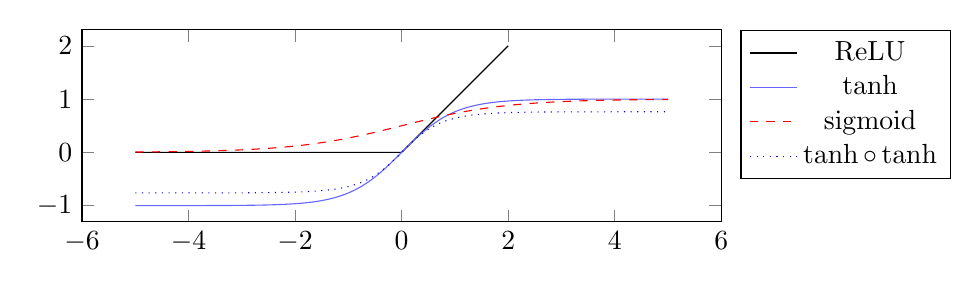
\begin{tikzpicture}
  \begin{axis}[
%    trig format plots=rad,
%    axis equal,
    axis equal image,
%    hide axis
%    thick, %affects border as well as plots
    width=0.8\textwidth, %even if the legend is outside, this only affects the axis object's scale, even though scale only axis is false (i.e. false means include just the axis labels etc)
    legend style={
      %legend pos=south east,
      legend pos=outer north east,
      %at={(0,-0.2)},
      %anchor=north west
    }
    ]
    \addplot [domain=-5:2, samples=200, black] {max(0,x)};\addlegendentry{ReLU}
    \addplot [domain=-5:5, samples=400, blue!60!] {tanh(x)};\addlegendentry{$\tanh$} %or semithick or something
    \addplot [domain=-5:5, samples=400, red, dashed] {1/(1+exp(-x))};\addlegendentry{sigmoid}
    \addplot [domain=-5:5, samples=200, blue, dotted] {tanh(tanh(x))};\addlegendentry{$\tanh\circ\tanh$}
  \end{axis}
\end{tikzpicture}

\caption{\label{fig:activations}Some important activation functions}
\end{figure}

\subsection{Convolutional}
Fully connected networks take their input to be $X=\mathbb{R}^{u_0}$ with no additional structure.
They know of no particular structure of the input space.
Often there is some structure which we want to be taken into account.
A common case is that we are given data in say $\mathbb{R}^{u_0^0}$ for each point on a lattice of shape $u_0^1\times u_0^2\times\dots\times u_0^d$.
Our data lives in the space $X=\mathbb{R}^{\prod_{i=0}^du_0^i}$.
Convolutional neural networks (CNNs\jind{CNN}) are a generalisation of fully connected neural networks which take this into account.
For example, if we are dealing with colour photographs of resolution $28\times28$ we would have $X=\mathbb{R}^{3\times28\times28}$, where we have a value for the brightness of red, green and blue at each pixel.
We want functions which treat pixels similarly to each other, and which treat neighbouring pixels similarly, to be favoured by the inductive bias of our model.
We want the model to be able to learn a function which doesn't change much if a picture is translated by about one pixel.

A convolutional network allows not just the input but other layers to have a grid structure.
The size of the array of values, or the number of units in layer $i$, $g_i(x,\lambda)$, is usually given by a sequence of numbers $u_i^0\times u_i^1\times\dots\times u_i^d$.
$u_i^0$ is known as the number of \emph{features} in the layer -- this is the number of values per point in space.
There are several common types of layers.
Two of the simplest are the convolutional and max pooling layers.
If layer $i+1$ is an $(l_1\times\dots\times l_d)$-\emph{convolutional layer} it contributes a vector $b_{i+1}\in\mathbb{R}^{u_{i+1}}$ and a (typically small) $u_{i}^{0}\times u_{i+1}\times l_1\times\dots\times l_d$-array $W_{i+1}$ to $\Lambda$.
Then, in a simple setup, the elements of the layer's outputs $g_{i+1}(x,\lambda)$ are the values of 
\begin{align}
  \sigma\Big(\sum_{j_0=0}^{u_{i}^0}\sum_{j_1=0}^{l_1}\cdots\sum_{j_d=0}^{l_d
 }(g_i(x,\lambda))_{(j_0,k_1+j_1,k_2+j_2,\dots,k_d+j_d)}(W_i)_{(j_0k_0j_1j_2\dots j_d)}+(b_i)_{k_0}\Big)
\end{align}
as $k_0$ ranges from 0 to $u_{i+1}^0$ and the other $k_p$ range from 0 to $u_{i+1}^p=1+u_i^{p}-l_p$.
There are numerous variations on this theme, for example treating the boundary differently or enforcing further sparsity on $W_{i+1}$.
The idea is that the new units at a point in space only depend on the values of the units in the previous layer near that point in space, and the manner of the dependence is the same over all space.
This layer is seen as analogous to the V1 cells in a visual cortex.
This is equivalent to a fully connected layer where the matrix $W$ is restricted to a very special sparsity pattern, and also that its nonzero values are repeated in a certain way.
% If layer $i+1$ is an $(l_1\times\dots\times l_d)$-\emph{max pooling layer}, then it contributes
A max pooling layer takes the maxima of each feature over a each of a grid of small cuboids which either cover each dimension or overlap in each dimension, thus preserving the number of features ($u_{i+1}^0=u_i^0$) but reducing the other dimensions.
It has no parameters. A typical such layer reduces the number of units in each spatial dimension by a factor of two.
The highest levels in a typical CNN typically take all the units to be a single vector and thus are fully connected, and so the output of the network happens in the same way as the FCNN\@.

\subsection{Recurrent neural networks}
The input being a sequence is an important case of a specially-structured input which it is important for the network to take into account.
A simple case is that for each example we are given data in say $\mathbb{R}^{u_0^0}$ for each of $u_0^1$ time points.
Our data lives in the space $X=\mathbb{R}^{u_0^0u_0^1}$.
We could be use a 1-D convolutional network (i.e.~one with $d=1$) in this case, but recurrent neural networks (RNNs\jind{RNN}) are an important alternative type of architecture in this case.
While convolutional and pooling layers allow the local spatial structure to be taken into account in the learning, RNNs force the temporal structure into the model, and explicitly globally, not just in a ``local'' way.
An RNN allows the network to allow earlier entries of the sequence to be taken into account when processing later entries.
Just like for fully connected and convolutional networks, the network is built from a sequence of layers.
The simplest RNN layer could take input as a sequence of $u_i^1$ values in $\mathbb{R}^{u_i^0}$ to output of the same number ($u_{i+1}^1=u_i^1$) of values in $\mathbb{R}^{u_{i+1}^0}$ % (with the time dimension unchanged )
Its parameters would be a weight matrix
 $u_{i-1}^0\times u_i^0$ matrix $W_i$, a second (square) weight matrix
 $u_i^0\times u_i^0$ matrix $\bar W_i$ for the recurrence, and a $u_i^0$-vector of biases $b_i$.
\begin{align}
  (g_{i+1}(x,\lambda))_1&=\sigma((g_i(x,\lambda))_1W_i+{}\phantom{(g_{i+1}(x,\lambda))_{t-1}\bar W_i+{}}b_i)\\
  (g_{i+1}(x,\lambda))_{\mathrlap{t}\phantom{1}}&=\sigma((g_i(x,\lambda))_{\mathrlap{t}\phantom{1}}W_i+           (g_{i+1}(x,\lambda))_{t-1}\bar W_i+b_i)&\text{for $t>1$}
\end{align}
(For a few paragraphs I am omitting the parameters $x$ and $\lambda$ from $g$).
Intuitively, what is happening here is that a learned map is converting a hidden state $(g_{i})_t$ to a new hidden state using one more piece of source data.
The hidden state can store a representation which knows about everything which has already been seen.

If we need to output one value for the whole sequence, the highest levels of the RNN will be fully connected, initialised from just the final timestep of the last recurrent layer, i.e.~$(g_{i})_{u_i^1}$.

\subsection{LSTM}
When trying to use RNNs when the sequence is long, it is hard for the early parts (low $t$) of the sequence to influence the final state, and thus there is a limit to what the network can learn.
The state has to be remembered through many multiplications by the matrix  $\bar W_i$.
For most values of $\bar W_i$ the derivative of $(g_i)_{u_i^1}$ with respect to an element in $(g_{i-1})_t$ for $t\ll u_u^1$ will be very large or very small.
This is called the problem of exploding or vanishing gradients.

% As a result, the network will not learn

Long-short term memory (LSTM, \cite{LSTM}\jind{LSTM}) is a variation of a recurrent layer which is designed to allow information to survive in the state across many timesteps.
There are two separate sets of units which operate in pairs.
To each output element $\big((g_i(x,\lambda))_{t}\big)_j$ is associated a memory cell
$(c_t)_j:=\big((c_i(x,\lambda))_{t}\big)_j$.
The layer needs parameters\footnote{Note that in this widely accepted notation, the \textbf{superscripts} $i$, $o$ and $f$ are decorations not variables nor placeholders.}
$u_{i-1}\times u_i$ matrices $W_i^f$, $W_i^i$, $W_i^o$ and $W_i^c$, $u_{i}\times u_i$ matrices $\bar W^f_i$, $\bar W^i_i$, $\bar W^o_i$ and $\bar W^c_i$, and
$u_i$-vectors $b_i^f$, $b_i^i$, $b_i^o$ and $b_i^c$.
The layer uses the sigmoid function, $\sigma'(x)=\frac1{1+e^{-x}}$ which is monotone increasing from $\mathbb{R}$ to the interval $(0,1)$. The normal activation function, $\sigma$, is usually $\tanh$.
They are evaluated for $t>1$ using temporary variables $f_t$, $i_t$, $o_t$ and $\tilde c_t$ as follows.
\begin{align}
  % trying to make everything line up exactly with phantoms/phanta is a bit of a pain here.
  % because W^f and W^{other letter} are lined up quite differently
\gdef\makevar#1{#1_t&=\sigma'((g_i(x,\lambda))_tW^{#1}_i+(g_{i+1}(x,\lambda))_{t-1}\bar W^{#1}_i+b_i^{#1})}  \makevar{f}\\
  \makevar{i}\\
  \makevar{o} \\
  \tilde c_t  &=\phantom{\sigma'}\mathllap{\sigma}((g_i(x,\lambda))_tW^{c}_i+(g_{i+1}(x,\lambda))_{t-1}\bar W^{c}_i+b_i^{c})\\
  c_t&=f_t\odot c_{t-1}+i_t\odot\tilde c_t\label{eq:forget}\\
  (g_{i+1})_t&=o_t\odot \sigma(c_t)\label{eq:output}
\end{align}
where $\odot$ denotes the Hadamard/entrywise product. To interpret these formulae for $t=1$, we think of $c_0$ and $(g_{i+1})_0$ as being 0.

It is hard to know exactly why a neural network is working, but there are aspects of the design of LSTM which make sense.
The usual interpretation of this is as follows.
We think of values which have passed through $\sigma'$ as being practically boolean 0/1 values.
The $c_t$ cells preserve information for many time steps.
A cell can be turned off, or made to ignore its existing value, by some timestep triggering the ``forget gate'', which means setting $f_t$ to 0%
\footnote{A model where $f$ is ``whether to forget'', with $f_t$ replaced by $(1-f_t)$ in \eqref{eq:forget}, would be totally equivalent.},
and can be given a new value, the calculated $\tilde c_t$ by the ``input gate'' $i_t$ being triggered.
Whether the value in a cell is actually used for output at a timestep is governed by the ``output gate'' $o_t$.
We can see that it is easy for a value in $x_t$ to affect a cell in $c_{t'}$ with $t\ll t'$ because it could be stored in some cell $c_t$ and then not be forgotten.
This is how the vanishing gradient problem is alleviated.


The long term information stored in the cells is separate from the immediate information stored in the outputs. Note that if $f$ manages to stay 0 and $o$ and $i$ manage to stay 1 then this is a vanilla RNN unit, albeit with the nonlinearity $\tanh\circ\tanh$, see \autoref{fig:activations}.

The only link between $(c_{\cdot})_j$ and $(g_\cdot)_{j}$ (which means that the cell and the hidden state of a unit are linked, and we don't just have a load of hidden states and a load of cells) is the final equation.

It is not clear that $\tanh$ is needed in both places, and it could easily be replaced with another activation function.

LSTM achieves impressive results in practice, though can take a long time to train.
There are many variations on LSTM which have been proposed.
It requires a very large amount of experimentation to be sure which modifications are real improvements.
There is also recent suggestion (e.g.~\cite{Are_LSTMs_DEAD} and \cite{NoRNN}) that for many current applications recurrent networks are not needed at all, because for many tasks their performance can be beaten by modern designs of 1D-CNNs, which are more efficient to train.


\subsection{Dropout and batch normalization}
% not something I play with, but something I use.
There are two very useful methods for improving the effectiveness of neural networks.
They have in common that although they do not change (or hardly change) the form of $\tilde f$, a variant of $\tilde f$ is actually used during training.

In dropout \cite{dropout1,dropout2}, we may pick a \emph{dropout probability} $p\in(0,1)$, typically $0.5$, for a weight matrix $W$ somewhere in the definition of $\tilde f$.
Then, for each training example $x\in X$ used in training we generate a matrix $B$ of i.i.d.~$\text{Bernoulli}(p)$ random variables and replace $\tilde f(x,\lambda)$ with its value where $W$ has been replaced with $\frac1p W\odot B$, where $\odot$ denotes the elementwise or Hadamard product. 
(In \cite{batchwiseDropout} we suggest picking a single $B$ for a whole minibatch, which is an additional optimization to consider.)
%which has not been used in any of these experiments.)
The effect of this tends to be that learning is slower but generalisation is better. This is thought to be partly because two units cannot train together.

%pity I can't use $x$ here like the normal paper
Applying batch normalisation \cite{batchNorm} to a scalar value $z$ somewhere in $\tilde f$ means adding two scalars $\beta$ and $\gamma$ to the set of parameters to learn, $\Lambda$, and replacing $z$ in the definition of $\tilde f$ with $\gamma\frac{z-\mu_{\mathcal{B}}}{\sqrt{\sigma^2_{\mathcal{B}}+\varepsilon}}+\beta$ where $\varepsilon$ is a small fixed parameter.
During training, $\mu_{\mathcal{B}}$ and $\sigma^2_{\mathcal{B}}$ are the mean and standard deviation of $z$ across the minibatch being used (which will depend on the current values of both  $\chi$ and $\lambda$), and during testing/inference they are estimates of $z$ across the whole training set.
Normally this will be applied across all the activations in a layer, possibly for every layer.
In the case of convolutional and recurrent layers, the parameters $\beta$ and $\gamma$ for all the units which share the same weight will usually be shared.
For example the same unit being calculated at different places in the input will share these values. That way the symmetrical structure of the layer is not broken, and the same unit always sees the same type of input.

In the experiments our focus is on the use of the signature, and I've kept the network architectures very simple. In practical applications, these two techniques are likely to be very important for getting the best results.
\subsection{Initialisation}
\label{sec:initialisation}
% movee this around
The algebraic formulae defining a neural network model are unchanged if they are composed with an affine transform of the basic data: this is just equivalent to changing the weights and biases.
% At first glance, this means that we would not need to worry about the scale of
In training the weights are initialised only one way, however.
As a consequence, if extreme translations of the data are necessary to find meaningful patterns, these translations will take a long time to be found.
In order for all the units to have a chance to be useful, it makes sense to ensure that all the inputs are about the same size (e.g.~around $[-1,1]$ or $[0,1]$) and to initialise the random weight matrices to keep this approximate scale for all units.
Much effort has been put into making this work well, famously \cite{Glorot,He,init}.

When classifying Chinese characters, which are all on the same scale, I might want to use coordinates as features.
We rescale the bounding box to $[-1,1]^2$ so that these coordinates can all be in a sensible range.

Elements of the signature or log signature of a path at level $m$ scale like $\mathrm{length}^m$ when the path is scaled.
%It is easy to 
When using the signature as input to a neural network the scaling has to be taken into account.
Once a feature is chosen, an easy approach is to find the mean and variance of that feature over a large random sample of training data and then use the mean and variance to always scale the feature to aim at a mean of 0 and a variance of 1.
Others have had other approaches to this.
One suggested by \cite{LengthNormalized}, around equation~(5), is equivalent to enlarging the path to a fixed length before taking the signature.

\section{Symmetries for handwriting}
In online character recognition each character is given as a sequence of strokes, each stroke is given as a sequence of coordinate points. In our work, we regard these points just as a 2D path.
That means we are deliberately ignoring other facts about the data which may come from the pen, for example the time of each coordinate point and the force in the pen.
For readers, and therefore potentially in the education of writers, the time spent on each part of the stroke is not important, so ignoring this is a good idea.
There are usually many more given points in a stroke in each important turn.
Given this as our approach, there is an approximate invariant, in that single points can be added or removed along the path and the character will remain similar.
If the stroke's signature is taken as the only representation of the stroke, then we have a method which automatically works with this invariant. This is a consequence of the fact that the signature of a path is independent of its parametrisation.
The other methods of representation I have attempted needed to explicitly bear in mind this invariant.

Chinese characters stand alone enough that it is meaningful to want to classify them individually.
The absolute size of a character is generally not important for distinguishing Chinese characters. 
(There could be scripts where this is not the case.)
%, for example `c' and `C' may not be distinguishable in isolation in English, or the triple Yud /Nun sofit / Vav which may only differ in Hebrew handwriting up to size). %\includegraphics{Hebrew_letter_Vav_handwriting.svg}
\iffalse
\begin{tikzpicture}
\begin{scope}[scale=0.015,yscale=-1]
%These are svgs of the 3 hebrew letters from wikipedia with the starting point modified.
  \filldraw svg{m136,549c-10.9-4.33-11.9-16.2-9.83-28.4,2.53-14.7,7.93-26.7,9.68-42,4.91-42.8,18.9-94.2,5.15-136,0-13.6-0.934-32,10.4-41.2,22.2-5.69,22.6-2.65,24.9,11.7,2.18,13.7,1.91,28.6,2.6,42.5-2.89,37.6-8.06,73.6-13.6,111-1.88,12.7-4.89,25.1-6.42,37.7-2.65,22,1.65,45-22.9,45z};
  \filldraw svg{m294.9,781c-12.8-6.42-18.7-20.8-20.8-34.3-0.548-3.39,0.711-4.58,3.54-11.4,6.85-16.6,6.53-26.5,13.1-47.6,4.94-16.5,9.12-45.5,13.3-77.1,8.38-64.1,17.1-116,29.4-179,4.92-25.3,9.13-54.5,6.58-60.7,0-19.6,3.55-51.8,23.6-61.8,7.92-3.95,8.68-1.7,11.9,5.97,1.33,3.17,2.41,6.57,3.67,9.76,0,18.9-3.06,37.9-6.59,56.9-4.74,25.6-8.99,50.7-14.5,76.1-17.1,79-21.6,149-39.6,229-3.72,16.4-9.65,30.5-9.59,47.2,0.0707,17.8-0.989,47.6-14,47.6z};
\filldraw svg{m541,387c-9-10-5-24-2-37 2-8 3-14 5-22 3-11 4-15 14-16 8-1 10-1 16,4 16,15 5,22-1,38-2,6-3,11-6,17-4,7-8,14-14,17-5,3-8,3-12-1z};
\end{scope}
\end{tikzpicture}
\fi
We therefore scale the character, preserving aspect ratio, to occupy a standard square, in particular $[-1,1]^2$.
This means that we will have no trouble with writers who chose to write in different sizes.

Small distortions in how a path looks are invariants for characters. Data augmentation is needed to take advantage of this, and doing so is needed to get good results on the CASIA data, but experimenting with augmentation is not my aim. I stick with a single method of augmentation which performs the following to each character, which works well, and which I inherited from Ben Graham.
The character is enlarged by a separate uniformly random factor in $[0.7,1.3]$ in the vertical and horizontal directions.
Then $\alpha$ is picked uniformly random in $[-0.3,0.3]$ and one of the following three things is picked to happen uniformly at random: (1) the character is rotated by $\alpha$ radians, (2) the character is horizontally sheered by $\alpha$, (3) the character is vertically sheered by $\alpha$. Then the character is scaled to lie within a fixed bounding box.
%function distortCharacter

\section{Chinese handwriting recognition results}
\label{sec:chinese}
Here I present some highlights of experiments attempting to learn the CASIA data with signatures and RNNs. 
The aim is to do well at this complex path classification task using a fast, smaller model.
A character is not a single path, it is a series of paths, one for each stroke. 
We come up with some way to use the signature to form a representation of a character which we feed to a traditional classifier.
Training as we did on a single desktop with a single graphics processing unit (GPU,\jind{GPU})\footnote{Originally designed for graphics, a piece of commodity hardware which is commonly and effectively used for training neural networks in addition to the central processing unit(s) (CPU\jind{CPU}) in each computer.} it is generally the case that the training time is dominated by the neural network operations on the GPU\@. 
Calculating minibatches with these representations on CPU-only background threads, for example using \ii, was fast enough that the GPU was continuously using the minibatches for training.
This indicates that further optimising the signature calculations would not significantly speed up this training.

\subsection{Signatures of each stroke}
The simplest method is to make a representation of each stroke and use the sequence of these representations as the input to the RNN\@. The signature alone would not make a good representation, as the network would not then have any indication of the relative locations of the strokes, which is important. We therefore use the starting point and the signature as the representation. We feed this to a  simple 1-layer LSTM, with the architecture shown in \autoref{fig:strokesig}. We trained the network with the common method Adam \cite{Adam} with its default parameters.

Because all the strokes are not much longer than a line in the bounding box, it was not necessary to normalise the signatures. In all these cases, the network was fully trained after 5 epochs which took about an hour. The final test accuracies are shown in \autoref{tab:strokesigres}. We see that the signature contains some useful information about the stroke. The method does not reach anywhere near useful accuracy.

\begin{figure}
\centering
%\begin{center}
\begin{tikzpicture}[framed,background rectangle/.style={draw,very thin,rounded corners}]
\node (inp) {\textsc{input}};
\node[draw,rectangle,above =1 of inp] (l1) {LSTM layer};
%1081344 when level=2
%\node[above of = l1] (o1) {\rlap{\ $1024\times(\text{number of strokes})$}};
\node[draw,rectangle,above =1 of l1] (l3) {forget all but last timestep};
%\node[above of =l3] (o3) {\rlap{\ 1024}};
\node[draw,rectangle,above=1 of l3] (l4) {dense layer {\parameterSize(3848875 parameters)}};
\node[draw,rectangle,above=0 of l4] (s4) {softmax};
\node[above = 1 of s4] (o4) {\textsc{output}};
\draw[-Latex] (inp)--node[right](extreme){\parameterSize $(\text{feature length})\times (\text{number of strokes})$}(l1);
\draw[-Latex] (l1)--node[right]{\parameterSize $1024\times(\text{number of strokes})$}(l3);
\draw[-Latex] (l3)--node[right]{\parameterSize 1024}(l4);
\draw[-Latex] (s4)--node[right]{\parameterSize 3755}(o4);
%The next two lines are just to add space to the left of the diagram
%so that the main arrows are roughly in the middle
\coordinate (far left) at ($(extreme.east)!1.7!(l1)$);
\node at (far left) { };
\end{tikzpicture}
%\end{center}
\caption[Signatures of each stroke LSTM network schematic.]{\label{fig:strokesig}Schematic diagram of  LSTM network architecture for signatures of each stroke. The data shapes are indicated on the arrows.}%Numbers of parameters are indicated in circles.}
\end{figure}

%size of LSTM layer:
%def f(m,n):return 4*(n*m+n*n+n)
\begin{table}
\centering
%  \begin{center}
    \begin{tabular}{ccccc}
      \hline
      Signature level&representation length&Total parameters&test accuracy\\
      \hline
      none&2&8 055 467&0.267\\
      1&4&8 063 659&0.493\\
      2&8&8 080 043&0.576\\
      3&16&8 112 811&0.630\\
      4&32&8 178 347&0.658\\
      \hline
    \end{tabular}
%  \end{center}  
  \caption[Results for signatures of each stroke]{Results summary on CASIA1.1 of training LSTM on signatures of each stroke}
  \label{tab:strokesigres}
\end{table}


\subsection{Signatures of local segments}
This is a simple and more successful representation method of a character, which first converts the character to a single 3-dimensional path.
I discussed a few methods for making a single 3-dimensional path from a character in \cite{handwriting}. 
A basic method is to add a ``pen dimension'' which is 0 on each stroke (pen down) and 1 on an added straight line (pen up) between the endpoints of the strokes. 
These 3D paths vary in their total length. 
A  basic step is to chop the paths into segments of equal length. 
This length includes the length expended in the pen direction, otherwise the interpolation can produce weird artefacts. This makes it a bit more likely that a split in a path will happen at a pen lifting.
We experimented with overlapping the segments, but this was not clearly advantageous.
We use this split of the character as the time dimension of the RNN, picking some representation of each segment. 
Different characters will have different lengths, but the LSTM requires a whole minibatch to have the same time length, so we pad backwards in time with zeros.

A simple and effective representation is the starting point of the segment concatenated with the signature of the 3-dimensional path which is that segment up to some level.
We considered adding the bounding box or centroid of that segment but it did not obviously help.

In these comparisons, we split the characters into segments (after scaling) of length 0.4.
Different characters have different numbers of segments, with the maximum being around 115.
%On average, the number of segments is therefore %%%%%%%%%%
%Comparisons were made here using two LSTM layers of 512 units each, the Adam optimizer with the default parameters, which is joined to a single Dense layer. 
The architecture is %shown in \autoref{fig:logsigpen}.
just the same as for the signatures of strokes case, except the time dimension is now ``number of segments'' note ``number of strokes''.
%Because the paths have been normalised, we were able to do these experiments without scaling the inputs here.
Again, we used Adam with default parameters and we were able to do these experiments without scaling the inputs.
Beyond level 4 the representation of a character is far too large to learn from efficiently. Level 4 is already rather large.
We observe that this method is promising.

\iffalse
\begin{figure}
\begin{tikzpicture}
\node (inp) {$(\text{feature length})\times (\text{number of segments})$ input};
\node[draw,rectangle,above of=inp] (l1) {LSTM};
\node[draw,circle,right=0mm of l1] {$\dagger$};
%1081344 when level=2
\node[above of = l1] (o1) {\rlap{\ $512\times(\text{number of segments})$}};
\node[draw,rectangle,above of=o1] (l2) {LSTM (2099200 parameters)};
\node[draw,cloud ignores aspect,cloud,right=0mm of l2,inner sep=0mm] {2099200};
\node[above of = l2] (o2) {\rlap{\ $512\times(\text{number of segments})$}};
\node[draw,rectangle,above of=o2] (l3) {forget all but last timestep};
\node[above of =l3] (o3) {\rlap{\ 512}};
\node[draw,rectangle,above of=o3] (l4) {dense layer};
\node[draw,circle,right=0mm of l4,inner sep=0mm] {1926315};
\node[draw,rectangle,above=0mm of l4] (s4) {softmax};
\node[above of = s4] (o4) {3755 output};
\draw[-Latex] (inp)--(l1);
\draw[-Latex] (l1)--(l2);
\draw[-Latex] (l2)--(l3);
\draw[-Latex] (l3)--(l4);
\draw[-Latex] (s4)--(o4);
\end{tikzpicture}
\caption[Schematic diagram of  LSTM network architecture for signatures of local segments.]{\label{fig:logsigpen}Schematic diagram of  LSTM network architecture for signatures of local segments. 
Numbers of parameters are indicated in circles.}
\end{figure}
\fi
%2 512 layers
%m=2 5106859 totalparams

%now it's 1 layer with 1024 units
%m=1 have 
%m=2 have 4259840+3848875=8108715
%m=3 have 4370432+3848875=8219307

\begin{table}
\centering
%\begin{center}
    \begin{tabular}{ccccc}
      \hline
      Signature level&\multicolumn{1}{p{2.5cm}}{\centering representation length}&\multicolumn{1}{p{2cm}}{\centering Total parameters}&time (hr)&test accuracy\\
      \hline
      none&3  &8 059 563&14.9&0.909\\
      1   &6  &8 071 851&15.6&0.933\\
      2   &15 &8 108 715&15.6&0.945\\
      3   &42 &8 219 307&15.8&0.951\\
      4   &123&8 551 083&18.5&0.947\\
      \hline
    \end{tabular}
%  \end{center}  
  \caption[Results for signatures of local segments]{Results summary on CASIA1.1 of training LSTM on signatures of local segments. Training was for 10 epochs.}
  \label{tab:logsigpenres}
\end{table}
%Note to self: it's not stupid to include all 3 coordinates of the starting point of each
%segment. Some segments will begin with the pen up.

\section{Sketchnet}
\label{sec:sketch}
The Sketchnet dataset \cite{sketch} consists of hand-sketches of each of 250 classes of objects, like `tomato', `banana' and `TV' by 80 different writers. There is no standard train/test split, I take the first 40 of each for training and the last 40 for testing. This isn't comparable with others. 
Each stroke in the Sketchnet data is not given just as a series of points, but often includes a series of Bezier curves. The data thus appears to have been coarsened. I interpolate each given curve with ample points before doing anything else with the data, so that it is like the situation with CASIA data.

Unlike characters of handwriting, a flip in a vertical axis is a reasonable invariant for sketches and so I include such a flip with probability $\frac12$ in the data augmentation.

There has been much work on this type of human sketch recognition, most prominently Google's ``Quick, draw''\footnote{\url{https://quickdraw.withgoogle.com}} which went viral in 2017. The methods used were not released, but when I saw this work I knew they had much more data and much more accuracy than I could hope for.
Using a similar signatures of local segments method as for the RNNs with CASIA, and with very little tweaking, I got to a test error of 33\%.

\section{Signatures in LSTM}
\label{sec:lstmsig}
\def\inV{i}
\def\outV{f}
\def\inputindex{l}
Making models which are more efficient than LSTMs is something many people are trying.
LSTMs can take a long time to train, and although they perform very impressively they seem logically inefficient for a couple of reasons to my mind.\footnote{The thinking here is my woolly intuition, and is suffused with the traditional, perhaps lazy, anthropomorphism.}
First, that they have to learn these operations of ``whether to save'' and ``whether to forget'' individually, which is quite remote from the actual problem being solved.
Second, that if the thing they need to save is high dimensional they have to teach themselves into a state which allows a group of cells to cooperate.
We know that signatures provide a good summary of the shape of a path, and the history of something can sometimes be thought of as a path, and networks memory is just its choice of salient features of its memory, so we wondered whether we could  use signatures as this memory.
The signature would be an input to a cell of a RNN based on the history of that cell.
%Thinking about this is where the idea came from to somehow allow a signature of past start
Note in particular that \emph{this} effort is not trying to produce a network which is specially designed to handle curves or which is taking signatures of data as input, but rather we are trying to come up with something which solves the sort of problems a vanilla LSTM is used for, and is potentially a drop-in replacement, but is ultimately, hopefully, better in some way -- faster to train or smaller or more robust.
The signatures are taken internally in the network; the user would not need to know about them.
In this effort the derivatives of the signature are necessary because there are parameters in the calculation graph of the network which are affecting the input of signature calculations.
We tried several architectures to try to test out this type of idea, for example where a cell was given a signature of the graph of its activation through history as an input.

Only one type of architecture was successful in the most minimal way, namely that we could train the network to solve a toy problem.
This was suggested by Harald Oberhauser, and involves following the structure of the LSTM as closely as possible. 
For example, we want to separate the internal memory from the output of a layer, and we want to separate the space where the memory lives from the spaces of our layer's inputs and outputs.
The idea is that, for some $K$ and $m$, the memory is a signature of a $K$-dimensional path up to level $m$,
%The suggestion is to replace the memory cell with a signature - 
i.e.~a value in a truncated tensor space $T^{\underline m}(\mathbb{R}^K)$. We are not defining it by specifying the path of which it is the signature. We choose a configuration which will be the same as vanilla LSTM when $m=1$ but generalises it for $m>1$.

The way we forget is to collapse the signature in a chosen direction, either entirely or partially. The matrix of stretching by a factor $\lambda$ in the direction of the unit vector $\hat \inV$ is $(I_K-(1-\lambda)\hat \inV\hat \inV^T)$.
% and we apply this transformation to the signature by premultiplying each level $m$ by its $m$th Kronecker-product power. %the iterated Kronecker product $(I_K+(\lambda-1)\vec a\vec a^T)^{\otimes m}$. 
If we were to generate $\hat\inV$ on its own in the network by making a vector $\vec \inV$ and normalising it there would be a nasty discontinuity around small $\vec \inV$. It would be nicer to do something like using $\|\vec \inV\|$ to get $1-\lambda$ or (which looks nicer) $\sqrt{1-\lambda}$ so that small values of $\vec \inV$ don't do anything. But we don't want $1-\lambda$ to be bigger than 1. So we use $\tanh \|\vec \inV\|$ as $\sqrt{1-\lambda}$ to get the matrix $\left(I_K-\frac{\tanh^2\|\vec \inV\|}{\|\vec \inV\|^2}\vec \inV\vec \inV^T\right)$.
%Call this operation on signatures $\text{Forget'}_{\lambda,\vec a}(\cdot)$.
To apply this transformation to the signature we premultiply each level $m'$ by the matrix's $m'$th Kronecker-product power. Call $\vec \inV$ the \emph{forget-vector}, and this operation on signatures $\text{Forget}_{\vec \inV}(\cdot)$.\footnote{In practice, this uses the \texttt{sigscale} functionality of \ii.}

To save information, we concatenate a new segment onto the path -- i.e.~Chen product the stored signature with the signature of a chosen segment.\footnote{In practice, this uses the \texttt{sigjoin} functionality of \ii.} %I use $\otimes$ to represent the Chen product. 
We need to pick the new segment in a sensible way to maintain the scaling of the signature, so we always make the new segment be a unit vector. %Just picking a unit vector would do, but I think we also had simpler ideas for this when we spoke in Oxford -- I think one was making $K$ equal to $L$ and just using the inputs. So 
We let $\text{Add}_{\vec \outV}(S)$ be the signature obtained as the Chen product of $S$ and $\exp (\frac1{\|\vec \outV\|}\vec \outV)$

We call one of these stored signatures a \emph{signature cell}. There are clearly many variations which could be tried, but for these experiments we have only one of them in the whole layer. We call the number of hidden units in the layer $u_{i+1}^0$. %$P$
%, we have a choice about how to group them - should there be more than one of them  - having only one isn't stupid, they can store lots of information. For the moment, let's say there are $N$ of them (labelled with $n$), and they all have the same number $K$ of dimensions (labelled with $k$) and maximum level $M$. Let the signature cell have value $S_{nt}$. Let each signature cell have $P$ hidden units (labelled with $p$).

We can't have an equation like \eqref{eq:forget} for a signature cell because a linear combination of signatures doesn't produce a signature. A simple way to do some forgetting and adding is to always do the forgetting and then always concatenate something on.

How to generate output based on the signature -- in analogy with (\ref*{eq:output}) -- is not obvious. Having a parameter the shape of a signature and using it as a linear functional is out solution to this, although it does involve adding many extra parameters.

Putting things together, we have the following parameters for an input to our layer $i$ of shape $u_i^0\times u_i^1$. $K\times u_i^1$ weights matrices $W^f$ and $W^i$, $K\times u_{i+1}^0$ weights matrices $\bar W^f$ and $\bar W^i$, and length-$K$ biases $b^f$ and $b^i$. $u_{i+1}^0\times u_i^1$ weights matrix $W^o$, $u_{i+1}^0\times u_{i+1}^0$ weights matrix $\bar W^o$, and length-$u_{i+1}^0$ biases $b^o$ and $b^h$ (if $S$ doesn't include a fixed 1). Also $u_{i+1}^0$ signature-shaped parameters $V^h$ each of size $\frac{u_{i+1}^0((u_{i+1}^0)^m-1)}{u_{i+1}^0-1}$ -- another big matrix. 
We used a common scheme for initialising the parameters -- the biases were initialised at zero, and each weight matrix was initialised in the ``Glorot Uniform'' method built in to Keras -- each element being uniformly distributed in $[-\frac{\sqrt 6}{g},\frac{\sqrt 6}{g}]$ where $g$ is the sum of the matrix's last two dimensions. The following are the complete defining equations, note that the variables $p$ and $p'$ vary among the $u_{i+1}^0$ output units.
\begin{align}
\inV_{kt}&=\sum_\inputindex W^\inV_{k\inputindex} ((g_i)_t)_\inputindex+\sum_{p'} \bar W^\inV_{kp'}h_{p',t-1}+b^\inV_{k}&&\text{\parbox{1.4in}{\raggedright $k$th element of forget vector $\vec \inV_{t}$}}\\
\outV_{kt}&=\sum_\inputindex W^\outV_{k\inputindex} ((g_i)_t)_\inputindex+\sum_{p'} \bar W^\outV_{kp'}h_{p',t-1}+b^\outV_{k}&&\text{\parbox{1.4in}{\raggedright $k$th element of new information vector $\vec \outV_{t}$}}\\
o_{pt}&=\sigma\left(\sum_\inputindex W^o_{p\inputindex} ((g_i)_t)_\inputindex+\sum_{p'} \bar W^o_{pp'}h_{p',t-1}+b^o_{p}\right)&&\text{\parbox{1.4in}{\raggedright in [0,1], whether to output anything}}\\
S_{t}&=\text{Add}_{\vec \outV_{t}}(\text{Forget}_{\vec \inV_{t}}(S_{t-1}))\\
\tilde h_{pt}&=V^h_{p}\cdot S_{t}+b^h_{p}&&\text{\parbox{1.4in}{\raggedright\setstretch{1} dot product of signatures as potential output}}\\
h_{pt}&=o_{jt}\tanh(\tilde h_{pt})&&\text{output}
\end{align}
The structure of a single timestep of one of these LSTM signature layers is summarised in \autoref{fig:LSTMsig}.
\begin{figure}
\begin{tikzpicture}[font=\scriptsize,node distance=2.4cm,auto]
	\node(a) {Input and old output};
	\node(aa) [xshift=20em]{Old path/signature};
	\node(b) [below right of=a,text centered,xshift=3em]{Forget direction};
	\node(w) [below left of=b,text centered,node distance=2em]{Whether to add};
	\node(s) [below left of=w,text centered,node distance=2em]{segment to add};
	\node(ww) [below left of=s,text centered,node distance=2em,yshift=-2em]{whether to output};
	\node(c) [below of=aa]{Contraction};
	\node(cc) [below of=c,node distance=3em]{Concatenation};
	\node(p) [left of=cc,node distance=6em]{Product};
	\node(nps) [below of=cc,node distance=3em]{new path/signature};
	\node(out) [below left of=nps,xshift=-3em,node distance=4em]{product = new output};
	\draw[-latex',very thick] (a) -> (b.north west);
	\draw[-latex',very thick] (a) -> (w.north west);
	\draw[-latex',very thick] (a) -> (s.north west);
	\draw[-latex',very thick] (a) -> (ww.north west);
	\draw[-latex'] (b) -> (c);
	\draw[-latex'] (aa) -> (c);
	\draw[-latex'] (c) -> (cc);
	\draw[-latex'] (w) -> (p);
	\draw[-latex'] (s) -> (p);
	\draw[-latex'] (p) -> (cc);
	\draw[-latex'] (cc) -> (nps);
	\draw[-latex'] (ww) -> (out);
	\draw[-latex',very thick] (nps) -> (out);
	\end{tikzpicture} 
\caption[Schematic of one cell of an LSTM layer with signature memory.]{\label{fig:LSTMsig}Schematic of one cell of an LSTM layer with signature memory. Bold arrows indicate that learned parameters are involved.}
\end{figure}


\subsection{Toy problem}
We wanted a very simple example problem to see if our new design of network could (a) learn anything and (b) have memory, i.e.~learn something which depends only on a long-term dependency in the data. We wanted the problem to be simple as the calculation is quite slow despite using \ii, because significantly it is happening on a CPU rather than a GPU\@. We came up with the following task, which  can also easily be solved with a traditional LSTM\@. The task is to distinguish between (category $A$) a random binary string of i.i.d.~Bernouilli$(0.5)$ zeros and ones, and (category $B$) a string which begins with a shorter length $v$ binary string and continues with the length $v$ partial sums mod 2. For example, the following are such strings with $v=4$.
\begin{align*}
0010\ 1001001001\\
1011\ 1101111011
\end{align*}
Distinguishing these requires remembering something for at least $v$ steps. 
Also it is not possible to distinguish the classes perfectly, because a random string may have the form of the other strings by chance, but this is a small effect.
For the experiments I had a single one of my LSTM-signature layers, of which the value of the timestep was passed to a dense layer with 40 ReLU units, which was connected to a single sigmoid output. A summary of the network in use is shown in \autoref{fig:toyLSTM}.
\begin{figure}
\centering
%\begin{center}
\begin{tikzpicture}[framed,background rectangle/.style={draw,very thin,rounded corners}]
\node (inp) {\textsc{input}};
\node[draw,rectangle,above =1 of inp] (l1) {LSTM signature layer};
\node[draw,circle,right=0mm of l1] {$\dagger$};
%\node[above of = l1] (o1) {\rlap{\ $(10\text{ or }30)\times20$}};
\node[draw,rectangle,above=1 of l1] (l2) {forget all but last timestep};
%\node[above of = l2] (o2) {\rlap{\ 20}};
\node[draw,rectangle,above=1 of l2] (l3) {dense layer};
\node[draw,circle,right=0mm of l3,inner sep=0mm] {840};
\node[draw,rectangle,above=0mm of l3] (s3) {ReLU};
%\node[above of =s3] (o3) {\rlap{\ 40}};
\node[draw,rectangle,above=1 of s3] (l4) {dense layer};
\node[draw,circle,right=0mm of l4,inner sep=0mm] {41};
\node[draw,rectangle,above=0mm of l4] (s4) {sigmoid};
\node[above = 1 of s4] (o4) {\textsc{output}};
\draw[-Latex] (inp)--node[right]{\parameterSize $1\times20$}(l1);
\draw[-Latex] (l1)--node[right]{\parameterSize $(10\text{ or }30)\times20$}(l2);
\draw[-Latex] (l2)--node[right]{\parameterSize 20}(l3);
\draw[-Latex] (s3)--node[right]{\parameterSize 40}(l4);
\draw[-Latex] (s4)--node[right]{\parameterSize 1}(o4);
\node[right=1.6in of l4]{
  \begin{tabular}{ccr}
$K=u_1^0$&$m$&$\dagger\;\;$\\
\hline
10&1&580\\
10&2&1580\\
10&3&11580\\
30&1&4740\\
30&2&31740\\
30&3&841740
  \end{tabular}
};
\end{tikzpicture}
%\end{center}
\caption[LSTM signature schematic]{\label{fig:toyLSTM}Schematic diagram of architecture used for training an LSTM signature layer on a toy model. 
The data shapes are indicated on the arrows. 
Numbers of parameters are indicated in circles.}
\end{figure}

Because this was just a proof-of-concept and unlimited data could be generated, there was no need to have separate train and test sets. We just had a very large training set, which is highly representative of the two classes. The general result was that these networks were able to learn, but took a long time to start learning in some cases. This 
seems to be because initialisation is hard to get right. 
The graphs show the accuracy over the whole training set of 11000 samples after each epoch (pass through the whole of the data).
In the experiments which I plotted, $v$ is 15 and so 15 of the $u_0=20$ units are always random, so it is not easy to memorise the members of category $B$ and memory of length 15 steps is requires.
In \autoref{fig:lstmsig201010} I show cases for $m=1,2,3$ for $K=u_1^0=10$, and in \autoref{fig:lstmsig203030} I show cases for $K=u_1^0=30$.

        \begin{figure}
	\includegraphics[width=0.85\textwidth]{lstmsig20_10_10}
          \caption[LSTM Signature training accuracy -- 10D with 10 hidden units]{Accuracy of the classification of training the LSTM Signature network on the toy problem after each epoch. The first 15 of the 20 characters are random. Signature level: blue 1, red 2, yellow 3. 10 dimensions with 10 hidden units.}
          \label{fig:lstmsig201010}
        \end{figure}
        \begin{figure}
	\includegraphics[width=0.85\textwidth]{lstmsig20_30_30}
          \caption[LSTM Signature training accuracy -- 30D with 30 hidden units]{Accuracy of the classification of training the LSTM Signature network on the toy problem after each epoch. 15 of the 20 characters are random. Signature level: blue 1, red 2, yellow 3. 30 dimensions with 30 hidden units.}
          \label{fig:lstmsig203030}
        \end{figure}

There is a lot of scope for playing with this model --- many parameters to tweak and various initialisations to try. If investing heavily into this, I would want to move the calculations onto a GPU for much more efficiency, and then try to learn a standard sequence modelling benchmark, such as the famous Penn Treebank. The success of this experiment is in showing that something can be learnt by a layer with a signature inside.
\endDocumentJR

\printindex
\printbibliography[heading=bibintoc]


\end{document}

